\documentclass[11pt,a4paper]{article}
\usepackage[utf8]{inputenc}
\usepackage[T1]{fontenc}
\usepackage[spanish,es-nodecimaldot,es-tabla]{babel}
\usepackage{lmodern}
\usepackage[margin=2.3cm]{geometry}
\usepackage{amsmath,amssymb}
\usepackage{graphicx}
\usepackage{booktabs}
\usepackage{longtable}
\usepackage{float}
\usepackage{array}
\usepackage{caption}
\usepackage{enumitem}
\usepackage{xcolor}
\usepackage{multirow}
\usepackage[most]{tcolorbox}
\usepackage[hidelinks]{hyperref}
\usepackage{url}
\urlstyle{same}
\captionsetup{font=small,labelfont=bf}
\setlist{itemsep=1pt,topsep=3pt}
\sloppy
\newcommand{\Erms}{E_{\mathrm{rms}}}
\newcommand{\emx}{e_{\max}}
\newtcolorbox{caja}[1]{colback=gray!8,colframe=gray!60,title={#1},fonttitle=\bfseries,coltitle=black,colbacktitle=gray!20}

\title{\textbf{Diseño de injertos vasculares multicapa que reproducen la curva tensión--estiramiento de cada arteria:\\ bases de materiales, láminas enteras, pared gruesa y una red neuronal}}
\author{Pablo Silvoni}
\date{11 de noviembre de 2026}
\begin{document}
\maketitle
\begin{abstract}
\noindent Un injerto vascular que se distiende distinto que la arteria que reemplaza favorece la trombosis y la hiperplasia de la íntima. Los métodos de diseño publicados ajustan un único número ---la compliancia de una arteria promedio---. Aquí se presenta un método para diseñar, paciente por paciente, un injerto multicapa que reproduzca la \emph{curva completa} de la arteria, con su forma de J. Cada material del injerto se idealiza como una fibra que no tira hasta un estiramiento propio (recta truncada), y la arteria se aproxima por una suma de esos materiales, elegidos una vez para toda la población, con a lo sumo 20 láminas por material. El método se valida primero sobre la curva tensión circunferencial--estiramiento circunferencial, $\sigma_{\theta\theta}(\lambda_\theta)$, que no depende de la presión ni de la geometría de la pared. Con 41 carótidas humanas (Masson et al.), el diseño entero minimax ---el mejor diseño entero que existe, por programación lineal entera--- cumple la meta (peor error $\le3$\,\% del rango) en los 41 sujetos con 6 materiales. Una sola red neuronal, que elige las láminas de cada material sabiendo las de los anteriores (red en cadena), con una salida ordinal que respeta el orden de las cantidades, y se entrena dentro de la franja de curvas de la población, su dominio de validez, da directamente las láminas enteras en una evaluación, sin optimizar: con una búsqueda de $\pm1$ lámina cumple la meta en los 31 sujetos de entrenamiento, en los 10 de prueba y en 50 de 63 curvas de otros tres estudios ---carótidas común, externa e interna, capas aisladas, pacientes con placa, mediciones in vivo---, con otras leyes constitutivas; el minimax cumple en 57 de esas 63, y en las demás ningún diseño entero llega a la meta. Luego el método se aplica a la curva presión--diámetro, para la que el injerto es un tubo de pared gruesa: diseñado con la ley de Laplace ningún sujeto cumple al fabricarse, mientras que con pared gruesa cumplen los 41. El diseño se vuelve un problema no lineal entero; como referencia se resuelve en tres pasos (arranque, mínimos cuadrados no lineales y minimax entero), que cumplen en los 41 sujetos. La misma red en cadena, con una cabeza más para el preestiramiento, da las láminas de cada capa en una evaluación: con una revisión de $\pm1$ lámina cumple en los 41 sujetos con 6 materiales y en 40 con 5, y con curvas medidas con ruido cumple en más sujetos que el minimax, con un peor caso menor.
\end{abstract}
\tableofcontents

%=====================================================================
\section{Introducción}
La falla de los injertos vasculares de diámetro pequeño (trombosis, hiperplasia de la íntima) se debe en buena parte a factores mecánicos: flujo perturbado, resistencia insuficiente y desajuste de compliancia entre el injerto y la arteria~\cite{ding}. En la aorta de cerdo, un injerto con una capa que iguala la compliancia mantuvo la presión de pulso, la velocidad de onda y la distensibilidad, que se deterioraron al quitar la capa~\cite{rovas25}; en ratas, un injerto con composición optimizada para la compliancia del vaso receptor siguió ajustado a las cuatro semanas, con menos inflamación y más músculo liso contráctil~\cite{furdella}. Igualar la mecánica de la arteria mejora el resultado.

Varios trabajos optimizan el diseño con ese fin: tiempo de entrecruzado y espesor de un biopolímero~\cite{harrison}, proporción y espesor de las capas de un injerto multicapa~\cite{tamimi}, un refuerzo de nitinol~\cite{rovas23} o una espiral de refuerzo~\cite{jiang}, y andamios degradables que se transforman en neovaso~\cite{szafron,hsu}. Todos ajustan \emph{un número} (compliancia o distensibilidad) de una arteria \emph{promedio}. La respuesta de una arteria, en cambio, tiene forma de J: blanda a bajo estiramiento, cuando trabajan la elastina y el músculo, y rígida a alto estiramiento, cuando se reclutan las fibras de colágeno~\cite{holzapfel,humphrey}. Un número no describe esa forma, y la forma cambia de un paciente a otro y de una arteria a otra.

Este trabajo diseña el injerto para que copie la \emph{curva completa} de \emph{cada} arteria. El método tiene dos niveles, que se presentan en ese orden:
\begin{enumerate}
\item \textbf{Nivel del material (validación).} La curva objetivo es la tensión circunferencial en función del estiramiento circunferencial, $\sigma_{\theta\theta}(\lambda_\theta)$. Es una propiedad del tejido: no depende de la presión, del radio ni del espesor de la pared, y por eso es común a cualquier arteria cuya pared tenga respuesta en J. En este nivel el injerto es una suma de materiales, el diseño es lineal y cada paso del método puede compararse con una solución exacta.
\item \textbf{Nivel del tubo (aplicación).} La curva objetivo es la presión que soporta la pared en función del diámetro. Aquí entran la geometría y el modelo de pared gruesa, el diseño deja de ser lineal y se usan las conclusiones del primer nivel.
\end{enumerate}
Las contribuciones son: (i) una base de materiales tipo fibra elegida una vez para toda la población; (ii) el diseño entero óptimo, con a lo sumo 20 láminas por material, por programación lineal entera (minimax); (iii) una sola red neuronal, en cadena y con salida ordinal, que da directamente las láminas enteras en una evaluación, validada por separado en sujetos de entrenamiento, de prueba y de otros tres estudios, dentro de un dominio de validez fijado de antemano; (iv) la demostración de que, a nivel del tubo, el diseño debe hacerse en pared gruesa, lo que lo vuelve no lineal entero; y (v) la misma red en cadena aplicada al tubo de pared gruesa, comparada con un procedimiento de optimización de tres pasos.

%=====================================================================
\section{Datos}\label{sec:datos}
\subsection{Ley constitutiva y sujetos}
Masson et al.~\cite{masson} midieron en forma no invasiva, a lo largo del ciclo cardíaco, el diámetro y la presión de la carótida común de 16 sujetos normotensos (NT) y 25 hipertensos tratados (HT), y ajustaron a cada uno un modelo de la pared íntima--media con tres aportes: elastina neo-Hookeana, cuatro familias de fibras de colágeno de respuesta exponencial (axial, circunferencial y dos diagonales a $\pm\alpha$)~\cite{holzapfel} y tono del músculo liso~\cite{rachev}. Con estiramiento axial $\lambda_z$ fijo e incompresibilidad,
\begin{equation}\label{eq:masson}
\sigma_{\theta\theta}-\sigma_{rr}=c\,(\lambda_\theta^2-\lambda_r^2)+\lambda_\theta^2\sum_{k=1}^{4}c_{1,k}E_k\,e^{c_{2,k}E_k^2}\sin^2\varphi_k+T_m\lambda_\theta\Bigl[1-\Bigl(\frac{\lambda_m-\lambda_\theta}{\lambda_m-\lambda_0}\Bigr)^2\Bigr],
\end{equation}
con $E_k=\lambda_k^2-1$, $\lambda_r=1/(\lambda_\theta\lambda_z)$ y $\lambda_k$ el estiramiento de cada familia ($\lambda_z$, $\lambda_\theta$ y $\sqrt{\lambda_\theta^2\sin^2\alpha+\lambda_z^2\cos^2\alpha}$). Los 14 parámetros de cada sujeto están en sus Tablas 2 y 4 (Anexo~\ref{sec:anexo}). Diez sujetos (4 NT y 6 HT) se reservan para prueba y no intervienen en ninguna elección del método.

\subsection{Curvas de tensión}\label{sec:sigma}
La curva objetivo del primer nivel es $\sigma_{\theta\theta}(\lambda_\theta)$ en el borde media--adventicia, en 999 valores de $\lambda_\theta$ entre 1,02 y 1,16, calculada con \eqref{eq:masson}; en ese borde la tensión radial está fijada por la condición de contorno de Masson et al., $\sigma_{rr}(r_m)=-P_a$, donde $P_a=a\,e^{\,b\,r_m/r_m(t_d)}$ es una presión de tipo perivascular que representa en un solo término la acción de la adventicia y del tejido perivascular sobre la media (sus Ecs.~10 y~12; $t_d$, la diástole). Así, $\sigma_{\theta\theta}=(\sigma_{\theta\theta}-\sigma_{rr})-P_a$, con $P_a$ en su valor diastólico, $a\,e^{b}$. Recalculada así, reproduce las curvas medias publicadas (Figs.~5a y 7a de~\cite{masson}) con un error cuadrático medio de 1,2 a 1,7\,\% de su valor medio, del orden del error de digitalización. Las 41 curvas tienen forma de J (monótonas y convexas) y van de 4,7 a 49\,kPa en $\lambda_\theta=1{,}02$ y de 54 a 290\,kPa en 1,16 (Fig.~\ref{fig:sigma}). En la figura se superponen las curvas medias publicadas por Masson et al.\ (Fig.~5a: jóvenes y mayores; Fig.~7a: normotensos e hipertensos), que caen sobre las curvas recalculadas. Como la presión se expresa también en forma relativa a 13,332\,kPa (100\,mmHg), la tensión se muestra además relativa a una tensión de referencia de 150\,kPa. En forma adimensional, $(\sigma-\sigma_{\min})/\Delta\sigma$, normotensos e hipertensos tienen casi la misma forma; la diferencia está en el nivel de tensión.

Dos curvas límite encierran a los 41 sujetos: $y_1$, una curva de la ley de Masson con parámetros dentro del rango de los sujetos, que parte de la menor tensión medida y queda debajo de todos, e $y_2$, el sujeto más rígido extendido hasta 300\,kPa. El \emph{espacio de trabajo} son 22\,500 curvas sintéticas de la ley de Masson dentro de esa franja, con parámetros de 2 a 4 sujetos de entrenamiento mezclados y perturbados, o sorteados entre el mínimo y el máximo de los sujetos.

\begin{figure}[H]\centering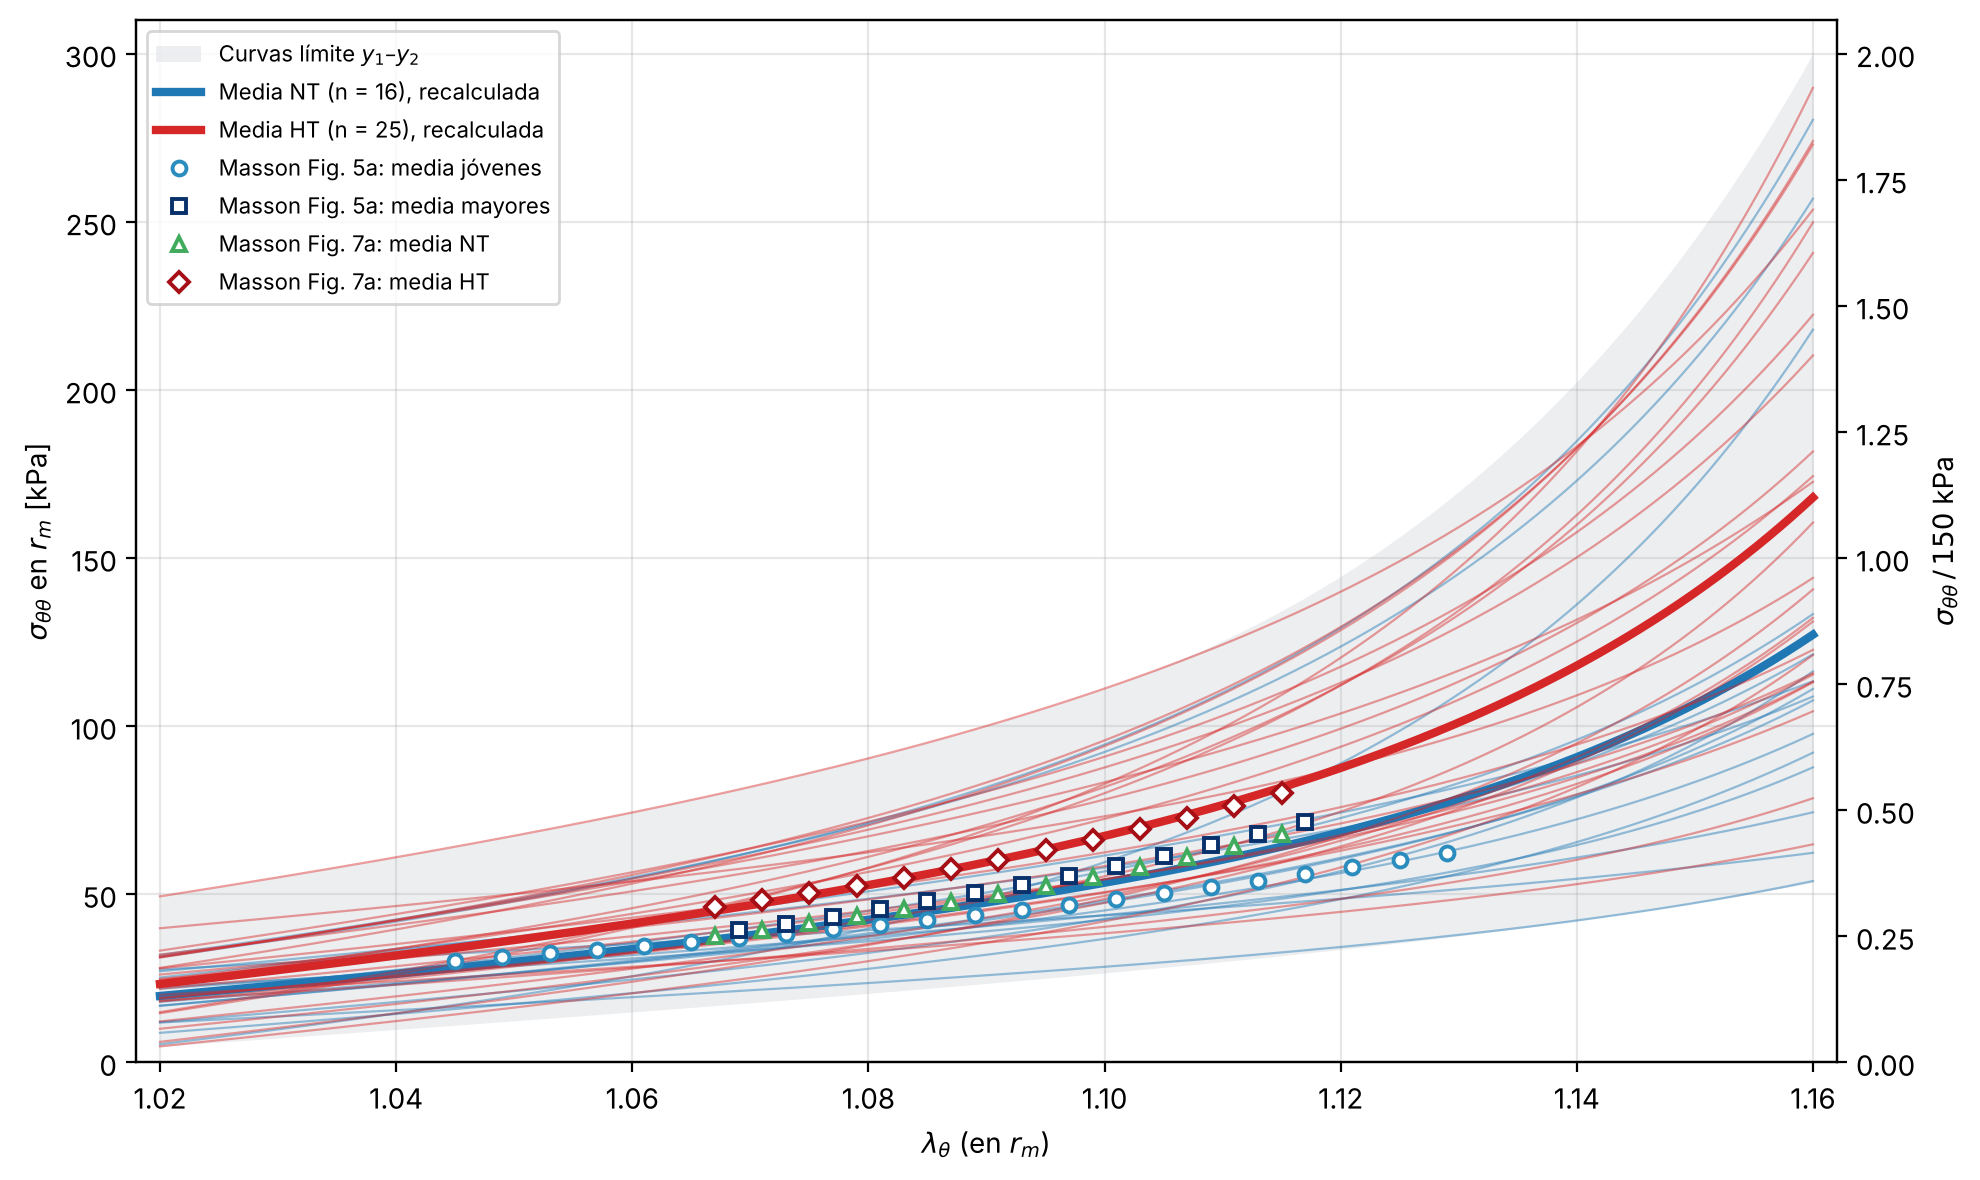
\includegraphics[width=\textwidth]{fig1_sujetos_sigma_v49.png}
\caption{Los 41 sujetos: tensión circunferencial en el borde media--adventicia; eje izquierdo en kPa, eje derecho relativo a 150\,kPa. Franja gris: curvas límite $y_1$--$y_2$. Azul: normotensos; rojo: hipertensos; trazo grueso: medias recalculadas de cada grupo. Marcadores: curvas medias digitalizadas de Masson et al.~\cite{masson}, Fig.~5a (jóvenes, mayores) y Fig.~7a (normotensos de 39 años o más, hipertensos); cubren el tramo de $\lambda_\theta$ que muestra el trabajo original.}\label{fig:sigma}\end{figure}

%=====================================================================
\section{Validación del método sobre la curva tensión--estiramiento}\label{sec:validacion}
\subsection{Materiales: rectas truncadas}
Una lámina del material $j$ aporta
\begin{equation}\label{eq:base}
A_j(\lambda)=S_j\,\max(0,\ \lambda-k_j):
\end{equation}
nada hasta su \emph{nudo} $k_j$, y luego una recta de pendiente $S_j$. Es la idealización de una fibra rizada que no tira hasta estirarse. El injerto es la suma $\sigma_{\mathrm{inj}}=\sum_j c_jA_j=A\,c$, con $c_j$ la cantidad de láminas de cada material y $A\in\mathbb R^{999\times N}$ la \emph{base}. Para nudos fijos, el problema es lineal.

\paragraph{Elección de los nudos.} Los nudos se eligen una sola vez, para toda la población, minimizando una \emph{función de costo} $\Phi(k)$ ---la llamamos así para no confundirla con la forma de J de las curvas--- que reúne tres exigencias sobre el espacio de trabajo y los sujetos de entrenamiento:
\begin{itemize}
\item \textbf{Precisión: CVaR 99\,\%.} Para cada curva se calcula el error máximo punto a punto del ajuste por mínimos cuadrados, $e_{\max}$ (ec.~\ref{eq:emax}). El CVaR 99\,\% (\emph{conditional value at risk}, valor en riesgo condicional~\cite{rockafellar}) es el promedio de $e_{\max}$ sobre el 1\,\% de las curvas con mayor error. A ese término se suma uno menor, 0,25 veces el NRMSE medio, para que el ajuste típico también mejore. Minimizar el promedio de todas las curvas dejaría sin control a las peores; minimizar solo la peor haría depender la elección de una única curva. El CVaR está entre ambos: atiende la cola de las peores curvas sin depender de una sola.
\item \textbf{Estabilidad: número de condición.} Con las columnas de $A$ escaladas a máximo 1, el número de condición es $\kappa(A)=s_{\max}/s_{\min}$, el cociente entre el mayor y el menor valor singular~\cite{trefethen}. Mide cuánto puede amplificarse, en las cantidades $c$, un error relativo de la curva: un error de 1\,\% en $y$ puede producir hasta $\kappa(A)$\,\% de error en $c$. Si dos nudos están muy juntos, sus columnas se parecen, $s_{\min}\to0$ y el diseño se vuelve inestable (cantidades grandes y de signo opuesto que se compensan). Se exige $\kappa(A)<30$; las bases adoptadas tienen 28,0 (6 materiales) y 19,0 (5).
\item \textbf{Signo.} Las cantidades del ajuste libre, $c=A^+y$, deben ser no negativas (con tolerancia de 0,01 lámina) en las 22\,500 curvas del espacio de trabajo, en los sujetos de entrenamiento y en las curvas límite, porque una cantidad negativa de material no se fabrica. La función $\Phi$ suma una penalización proporcional a las cantidades negativas. Como el signo de $c_j$ no depende de la pendiente $S_j$ (que solo escala la columna), esta condición queda fijada por los nudos.
\end{itemize}
En resumen,
\begin{equation}\label{eq:costo}
\Phi(k)=\mathrm{CVaR}_{99}(e_{\max})+0{,}25\,\overline{\mathrm{NRMSE}}+50\,\max\bigl(0,\ \kappa(A)-29\bigr)+1000\,\overline{n^{-}},
\end{equation}
donde $\overline{n^{-}}$ es la suma de las cantidades negativas de cada curva (en láminas), promediada sobre las curvas. Si los nudos no cumplen las restricciones de separación o de dominio (párrafo siguiente), $\Phi=10^{9}$: ese juego de nudos queda descartado.
La búsqueda es global por \emph{evolución diferencial}~\cite{storn}: una población de juegos de nudos candidatos se mejora generación a generación; cada candidato se perturba sumándole la diferencia entre otros dos, escalada, y el resultado reemplaza al candidato si da un $\Phi$ menor. No usa derivadas, que $\Phi$ no tiene (el $\max$, la ordenación del CVaR y las penalizaciones la hacen no diferenciable), y explora todo el dominio, por lo que no se queda en el primer mínimo local. El mejor candidato se refina con el método simplex de \emph{Nelder--Mead}~\cite{nelder}, que tampoco usa derivadas: mueve un poliedro de $N+1$ vértices por reflexiones, expansiones y contracciones hasta cerrarlo sobre el mínimo.

\paragraph{Restricciones de los nudos.} Los nudos 2 a $N$ quedan dentro del dominio, separados al menos 0,008 (si se juntan, $\kappa(A)$ crece) y el último a más de 0,012 del extremo 1,16 (si no, su material actúa en muy pocos puntos y no se distingue del resto). El primero, $k_1$, se busca entre 0,6 y 0,98, \emph{antes} del dominio, por una razón física: en $\lambda_\theta=1{,}02$ todas las arterias ya tienen tensión (de 4,7 a 49\,kPa), y en ese punto el único material que puede aportarla es uno que ya esté trabajando. Ese material hace el papel de la elastina, que sostiene carga con la arteria descargada. Un nudo $k_1<1$ significa que la lámina se monta preestirada: con $k_1=0{,}82$, en $\lambda=1$ ya está estirada $1/0{,}82=1{,}22$. El límite superior 0,98 asegura que esté activa en todo el dominio con margen. El inferior, 0,6 (preestiramiento de 1,67), acota la búsqueda a valores fabricables. Ninguno de los dos límites está activo en el óptimo ($k_1=0{,}82$ con 5 y con 6 materiales): la elección no depende de ellos.

\paragraph{Pendientes.} $S_j=\mathrm{PEND}_{\max,j}/20$, donde $\mathrm{PEND}_{\max,j}$ es la mayor pendiente que el material $j$ debe aportar en el espacio de trabajo: así ninguna curva necesita más de 20 láminas de un material. La escala no cambia la curva (lo que cuenta es $c_jS_j$), pero fija el tamaño de una lámina.

\begin{figure}[H]\centering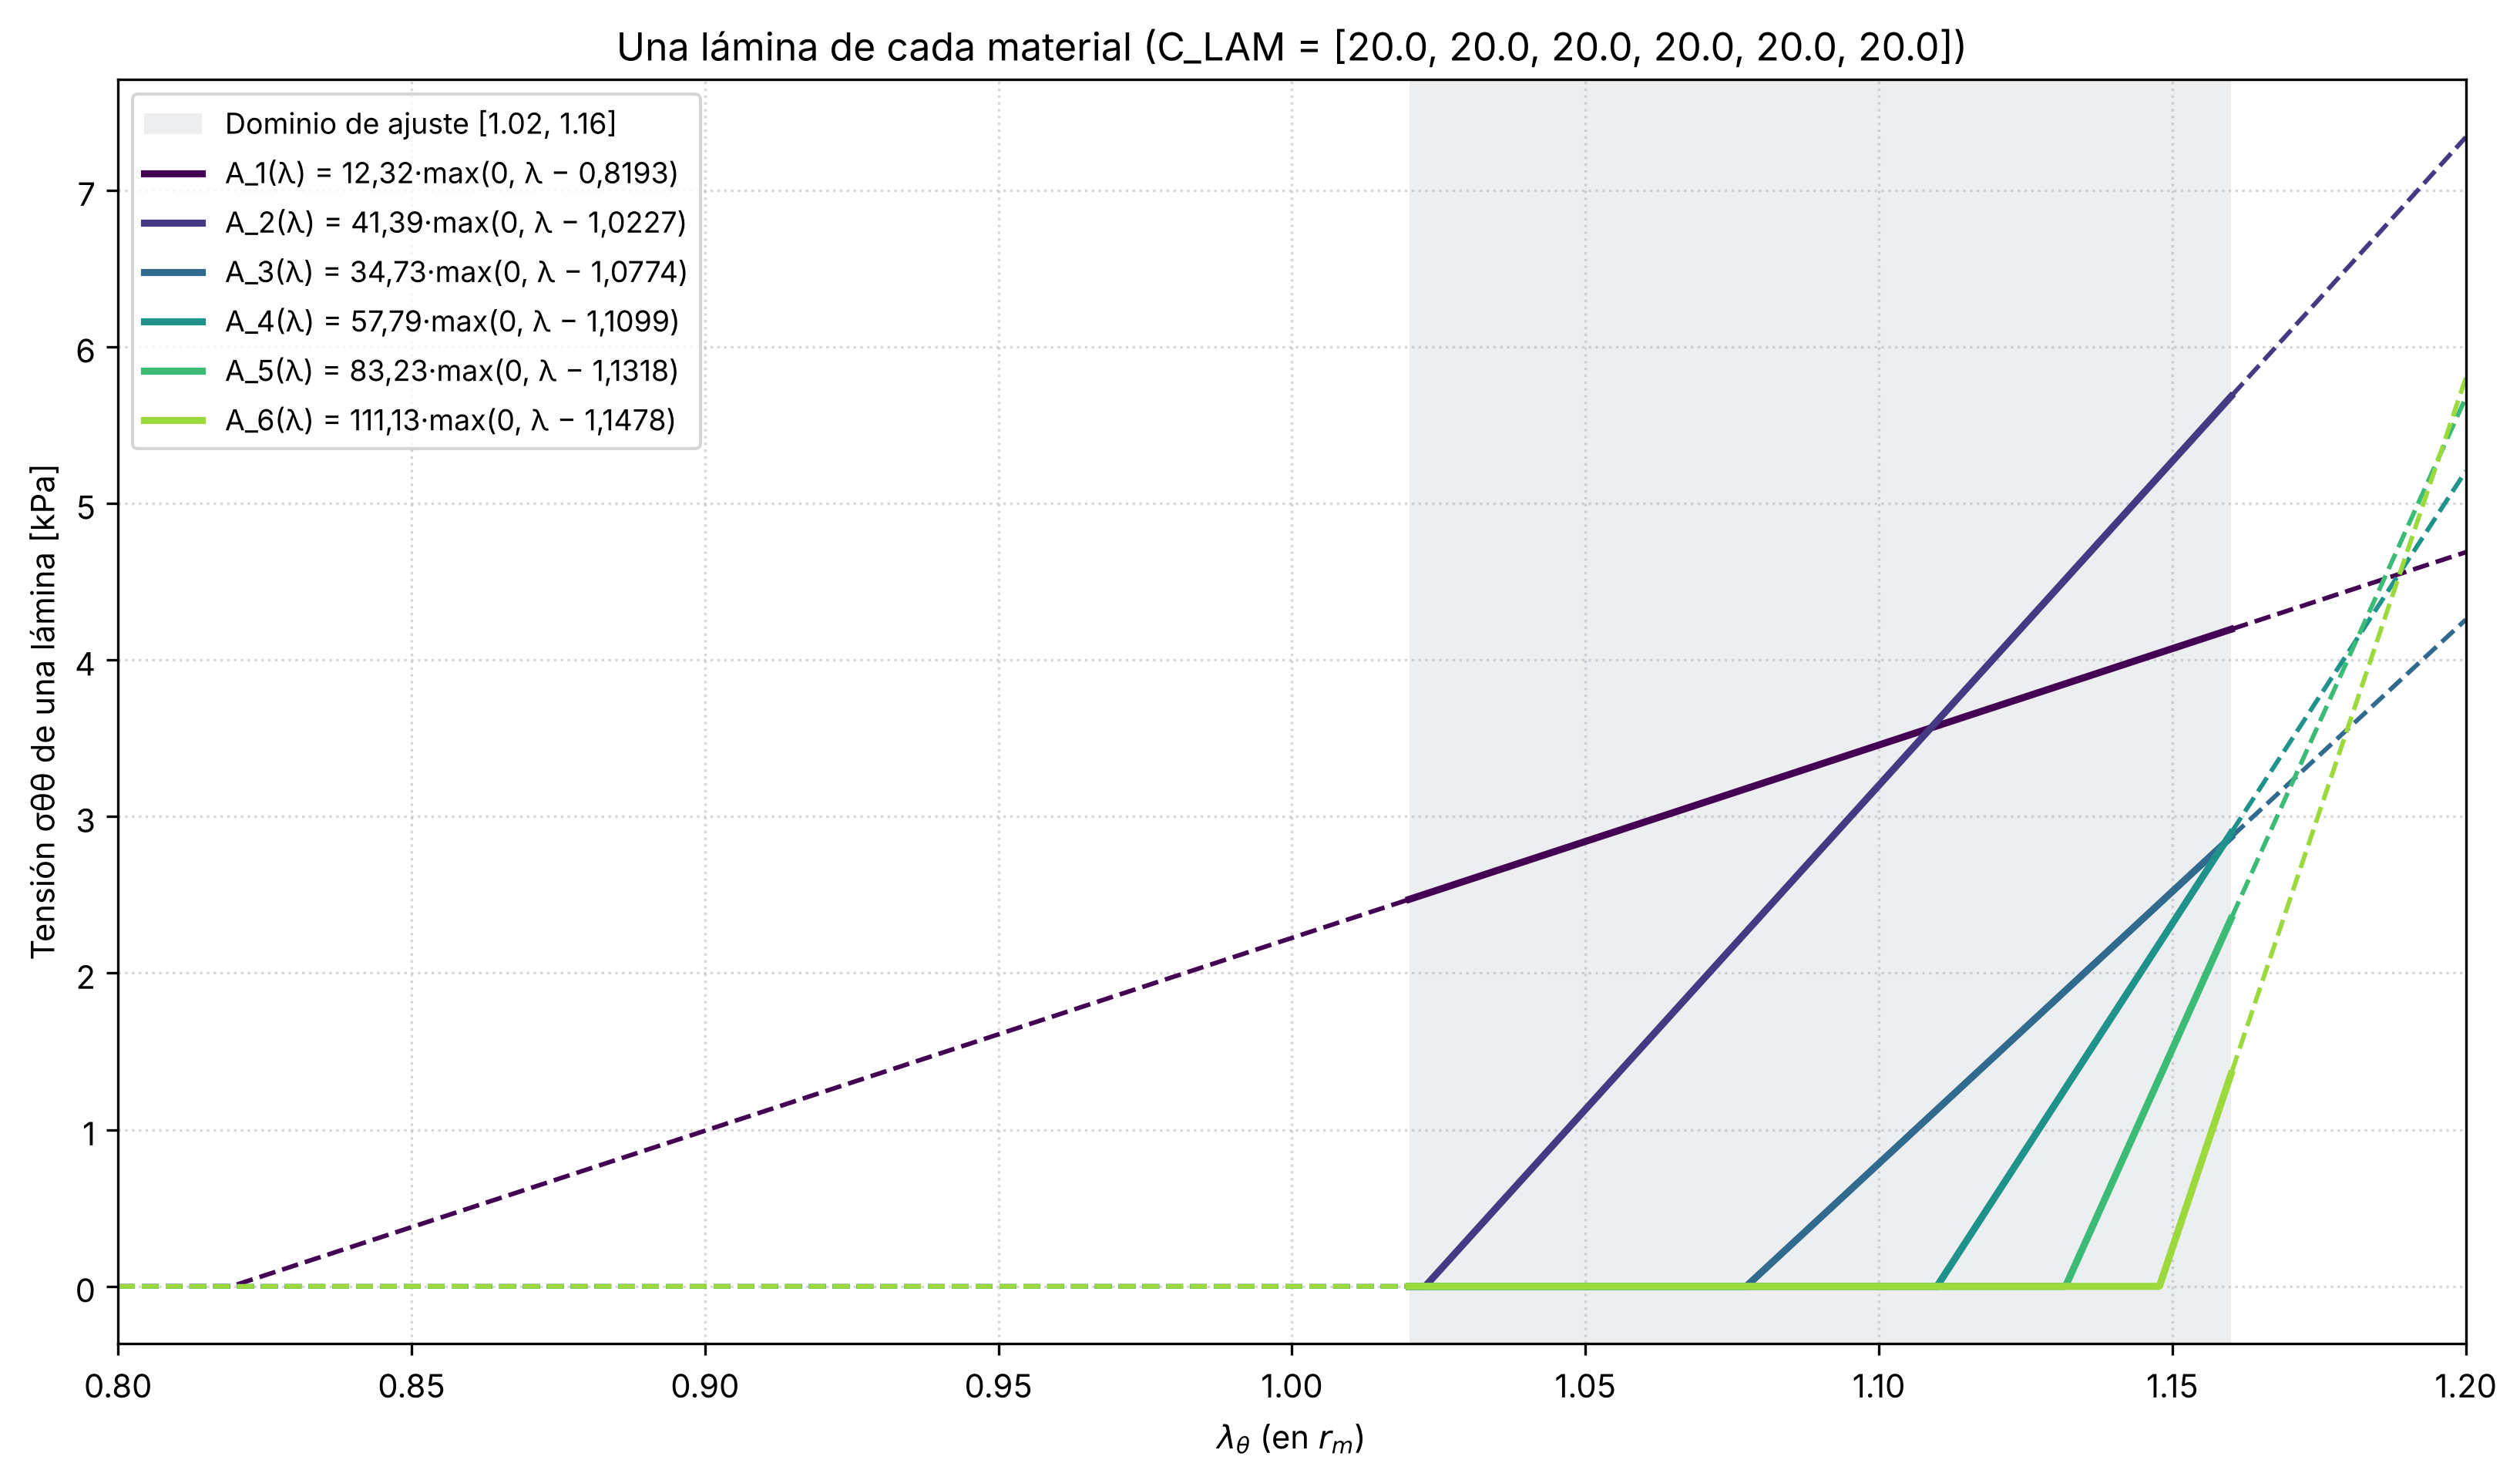
\includegraphics[width=0.85\textwidth]{bases_funcionales_v39_6.png}
\caption{La base de 6 materiales: una lámina de cada uno. El primer nudo (0,82) está antes del dominio, como la elastina, que ya trabaja con la arteria descargada; los demás se agrupan donde la curva arterial se curva más.}\label{fig:bases}\end{figure}

\begin{table}[H]\centering\small
\caption{Bases adoptadas: nudos $k_j$ y pendiente de una lámina $S_j$ [kPa].}\label{tab:bases}
\begin{tabular}{lcccccc}\toprule
 & 1 & 2 & 3 & 4 & 5 & 6\\\midrule
6 materiales, $k_j$ & 0,8193 & 1,0227 & 1,0774 & 1,1099 & 1,1318 & 1,1478\\
\phantom{6 materiales, }$S_j$ & 12,32 & 41,39 & 34,73 & 57,79 & 83,23 & 111,13\\\addlinespace
5 materiales, $k_j$ & 0,8228 & 1,0243 & 1,0881 & 1,1226 & 1,1447 & ---\\
\phantom{5 materiales, }$S_j$ & 12,56 & 43,57 & 51,92 & 88,74 & 129,08 & ---\\\bottomrule
\end{tabular}
\end{table}

\subsection{Métrica}
Para una curva objetivo $y$ con rango $\Delta=\max y-\min y$,
\begin{equation}\label{eq:emax}
e_{\max}=\frac{100}{\Delta}\max_i\,|y_i-\hat y_i|\quad[\%],\qquad E_{\mathrm{rms}}=\frac{100}{\Delta}\sqrt{\frac1n\sum_i(y_i-\hat y_i)^2},
\end{equation}
con $\hat y$ la curva del injerto. $e_{\max}$ es el peor punto; $E_{\mathrm{rms}}$ (o NRMSE), el apartamiento típico. Dividir por el rango hace el criterio igual de exigente con una arteria blanda que con una rígida. Meta: $e_{\max}\le3$\,\%. Todo diseño se evalúa contra la curva original.

\subsection{Cantidades reales: mínimos cuadrados}
Con la base fija, el mejor ajuste cuadrático es $c=A^+y$, con $A^+$ la seudoinversa de Moore--Penrose~\cite{penrose}, calculada por descomposición en valores singulares~\cite{golub}: exacta, única e instantánea. Con los nudos adoptados el número de condición es 19,0 (5 materiales) y 28,0 (6 materiales), debajo del umbral de 30, y ninguna curva del espacio de trabajo ni ningún sujeto necesita una cantidad negativa. El ajuste cumple la meta en los 41 sujetos, con peor error de 0,88\,\% (6 materiales; mediana 0,67\,\%) y 1,41\,\% (5 materiales; mediana 1,07\,\%), y en todas las curvas del espacio de trabajo.

\subsection{Láminas enteras: el diseño minimax}\label{sec:minimax}
Un injerto se fabrica con un número entero de láminas de cada material, $z\in\{0,1,\ldots,20\}^N$: a lo sumo 20 láminas por material, para no complicar la fabricación (con las pendientes adoptadas, ninguna curva del espacio de trabajo necesita más). El diseño entero de referencia no redondea ninguna solución real: busca directamente los enteros que dejan el túnel más angosto alrededor de la curva de la arteria,
\[
\min_{z,\tau}\ \tau\quad\text{s.a.}\quad -\tau\le\frac{100}{\Delta}\bigl(y_i-(Az)_i\bigr)\le\tau,\qquad z_j\in\{0,1,\ldots,20\},
\]
un programa lineal entero mixto (aproximación de Chebyshev~\cite{cheney} con enteros) resuelto por ramificación y acotación con HiGHS~\cite{highs}, en unos 50 a 65\,ms por curva. Sus únicos datos son la curva $y$ y la base $A$, y lo que se obtiene es el \emph{óptimo global}: el diseño entero de menor $e_{\max}$ que existe. Si el minimax no cumple la meta en una curva, ninguna combinación de láminas enteras la cumple. Por eso es la referencia contra la que se mide la red neuronal. Dentro del dominio de validez (Sección~\ref{sec:dominio}) el tope de 20 láminas no limita: sin tope, ninguna de las 63 curvas externas de la Sección~\ref{sec:externa} necesita más de 18 láminas de un material, y en ellas y en los 41 sujetos el $e_{\max}$ del minimax es el mismo con y sin tope (a menos de 0,01 punto).

\subsection{La red neuronal en cadena}\label{sec:enteros}
El minimax resuelve un problema de optimización entera por cada curva. Una red neuronal, en cambio, aprende de una vez la relación entre la curva y su diseño, y después da las láminas enteras de un injerto nuevo en una sola evaluación, sin optimizar. Para que dé enteros, la salida de cada material es \emph{ordinal}: en lugar de elegir una entre 21 categorías sin orden, la red responde, para el material $j$, las 20 preguntas ``¿lleva más de $k$ láminas?'' ($k=0,1,\ldots,19$), y el número de láminas es la cantidad de respuestas afirmativas. Así, la red sabe que 6 láminas está cerca de 5 y lejos de 20. Se usa una sola red, la de la Fig.~\ref{fig:cadena}, en todo el primer nivel.

\paragraph{Arquitectura.} Un tronco común, $999\to256\to128\to64$ (ReLU~\cite{relu}, normalización por capa~\cite{layernorm} y regularización L2 de $10^{-5}$), resume la curva en un vector $h$ de 64 números; la entrada es $\log(y+22)$ estandarizada. Hay una cabeza por material. La cabeza $j$ recibe $h$ y las láminas ya elegidas $n_1\ldots n_{j-1}$ (divididas por 20), pasa por dos capas (128 y 64 neuronas, ReLU) y calcula un único puntaje $s_j$. Las 20 preguntas comparten ese puntaje y difieren solo en un umbral propio, $P(n_j>k)=\sigma(s_j+b_{jk})$, con $\sigma$ la función logística~\cite{cao}; la respuesta es $\hat n_j=\#\{k:\ P(n_j>k)>1/2\}$. Se usa en orden ---material 1, después el 2 sabiendo el 1, y así hasta el último---, de modo que puede compensar entre materiales: si en uno puso una lámina de más, en el siguiente puede poner una de menos. Tiene 399\,928 parámetros con 6 materiales y 382\,628 con 5.

\paragraph{Cómo trabaja, paso a paso.} Una red neuronal común recibe la curva y entrega todas sus salidas de una vez. La red en cadena, en cambio, arma el diseño de a un material y usa sus propias respuestas como parte de la entrada. Por eso tiene dos entradas: la curva $\mathbf{y}$ y el \emph{vector de láminas decididas} $\mathbf{m}=(m_1,\ldots,m_N)$, con una componente por material ($N=6$ o 5, el número de materiales de la base). La componente $m_j$ vale $\hat n_j/20$ si las láminas del material $j$ ya se eligieron, y 0 si todavía no; se divide por 20, el máximo de láminas por material, para que quede entre 0 y 1 como el resto de las entradas. Por ejemplo, con 6 materiales, después de elegir 5 láminas del material 1 y 7 del 2, $\mathbf{m}=(5/20,\,7/20,\,0,\,0,\,0,\,0)$.
\begin{enumerate}[label=(\arabic*)]
\item \emph{Paso 1.} Todavía no se eligió nada: $\mathbf{m}=\mathbf{0}$. El tronco resume la curva en $h$, y la cabeza 1 responde las 20 preguntas ``¿más de $k$ láminas del material 1?''; $\hat n_1$ es la cantidad de respuestas con probabilidad mayor que 1/2.
\item \emph{Paso $j$, para $j=2,\ldots,N$.} Se vuelve a evaluar la red con la misma curva y con $\mathbf{m}=(\hat n_1,\ldots,\hat n_{j-1},0,\ldots,0)/20$, y se lee solo la cabeza $j$, que da $\hat n_j$. La cabeza $j$ mira únicamente las componentes $m_1,\ldots,m_{j-1}$, las de los materiales anteriores a ella.
\item Después de $N$ evaluaciones, $(\hat n_1,\ldots,\hat n_N)$ es el diseño.
\end{enumerate}
Por ejemplo, para el sujeto NT01 con 6 materiales, la cabeza 1 elige 5 láminas; la cabeza 2, sabiendo ese 5, elige 7; la 3, sabiendo 5 y 7, elige 5; y así hasta $[5,7,5,6,6,7]$ (Tabla~\ref{tab:suj6}). Como el tronco depende solo de la curva, $h$ es el mismo en los $N$ pasos: lo que cambia de un paso a otro es lo que la red sabe de los materiales ya decididos. Al entrenar no se hacen los $N$ pasos: cada cabeza recibe en $\mathbf{m}$ las láminas del minimax de los materiales anteriores y aprende a elegir la siguiente (punto~(c) del fundamento). La diferencia con una red común es la que hay entre acertar todas las cantidades a la vez, sin que un error pueda corregirse, y decidir cada material sabiendo cómo quedaron los anteriores, con la posibilidad de compensarlos.

\begin{figure}[H]\centering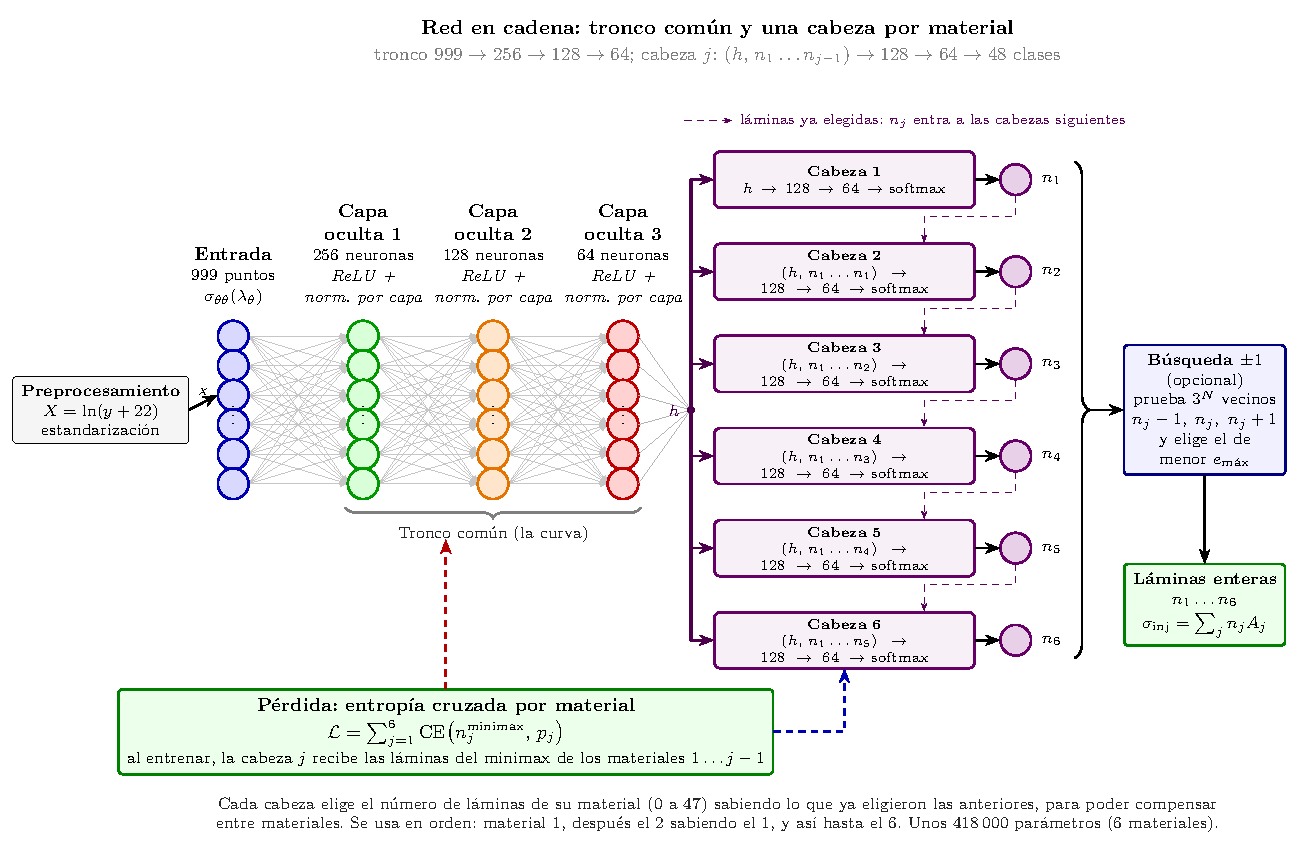
\includegraphics[width=\textwidth]{red_cadena_es.pdf}
\caption{Red en cadena para 6 materiales. Un tronco común ($999\to256\to128\to64$, ReLU y normalización por capa) resume la curva en el vector $h$; la cabeza $j$ recibe $h$ y las componentes $m_1\ldots m_{j-1}$ del vector de láminas decididas $\mathbf{m}$, es decir, las láminas que ya eligieron las cabezas anteriores divididas por 20 ($m_i=n_i/20$; flechas de trazos violetas), y responde las 20 preguntas ``¿más de $k$ láminas?'' con un puntaje y 20 umbrales; $n_j$, de 0 a 20, es la cantidad de respuestas afirmativas. La pérdida es la entropía cruzada binaria de esas preguntas contra el entero del minimax. La búsqueda de $\pm1$, opcional, revisa las $3^N$ combinaciones vecinas de la respuesta.}\label{fig:cadena}
\end{figure}

\paragraph{Fundamento de la red en cadena.} Se apoya en cinco resultados.
\begin{enumerate}[label=(\alph*)]
\item \emph{Aproximación universal.} Una red de capas con suficientes neuronas aproxima cualquier función continua en un conjunto acotado~\cite{cybenko,hornik,leshno}. Lo que aprende cada cabeza son las probabilidades $P(n_{ij}>k)$ de que la curva $i$ lleve más de $k$ láminas del material $j$, que varían en forma continua con la curva; el paso a un entero se hace recién al final, contando las respuestas afirmativas.
\item \emph{Regla de la cadena de la probabilidad.} La probabilidad de un diseño completo se descompone siempre, sin ninguna hipótesis, como
\begin{equation}\label{eq:cadena}
p\bigl(n_{1},\dots,n_{N}\mid\mathbf{y}\bigr)=\prod_{j=1}^{N}p\bigl(n_{j}\mid\mathbf{y},n_{1},\dots,n_{j-1}\bigr),
\end{equation}
y cada factor es lo que calcula una cabeza. Es la idea de los modelos autorregresivos~\cite{larochelle} y de las cadenas de clasificadores~\cite{read11}. Elegir cada material por separado supondría $\prod_j p(n_j\mid\mathbf{y})$, es decir, materiales independientes; como los materiales se compensan entre sí, esa hipótesis es falsa.
\item \emph{Máxima verosimilitud.} Para la curva $i$ y el material $j$, la etiqueta del minimax $n^{*}_{ij}$ se escribe como 20 respuestas, $y_{ijk}=1$ si $n^{*}_{ij}>k$ y 0 si no ($k=0,\ldots,19$), y la cabeza da $p_{ijk}=P(n_{ij}>k)=\sigma(s_{ij}+b_{jk})$. La pérdida es la entropía cruzada binaria sumada sobre las preguntas y los materiales, más una regularización L2 de los pesos del tronco:
\begin{equation}\label{eq:perdida}
\mathcal{L}(\theta)=\frac{1}{B}\sum_{i=1}^{B}\sum_{j=1}^{N}\sum_{k=0}^{19}\Bigl[-y_{ijk}\ln p_{ijk}-(1-y_{ijk})\ln(1-p_{ijk})\Bigr]+\lambda\sum_{W\in\text{tronco}}\lVert W\rVert^{2},\qquad \lambda=10^{-5},
\end{equation}
con $B=256$ curvas por lote. Cada término es menos el logaritmo de la probabilidad que la red da a la respuesta correcta de una pregunta: minimizar $\mathcal{L}$ es maximizar la verosimilitud de las respuestas del minimax, material por material y en el orden de~\eqref{eq:cadena}. Para entrenar cada factor de~\eqref{eq:cadena}, la cabeza $j$ recibe las láminas del minimax de los materiales anteriores (\emph{teacher forcing}~\cite{williams}); al usarla recibe las que eligieron las cabezas anteriores, $\hat n_{ij}=\#\{k:\ p_{ijk}>1/2\}$.
\item \emph{Representación compartida $h$.} Las $N$ cabezas resuelven tareas que dependen de la misma curva; un tronco común obliga a que $h$ guarde lo que sirve a todas y mejora la generalización frente a redes separadas~\cite{caruana,bengio13}. Las curvas dependen de pocos parámetros: la ley de Masson usa unos 8 por sujeto y el ajuste lineal reproduce cualquier curva del espacio de trabajo con $N$ coeficientes y error menor al 1\,\%. Los 64 números de $h$ alcanzan con margen. El tamaño 64, como 256 y 128, es una elección de diseño y no sale de un teorema.
\item \emph{Salida ordinal.} Las láminas son cantidades ordenadas: equivocarse por una lámina no es lo mismo que equivocarse por diez, pero una salida de 21 categorías sin orden trata igual los dos errores. Frank y Hall~\cite{frankhall} propusieron convertir una clasificación ordenada en una serie de preguntas binarias ``¿más que $k$?'', y Li y Lin~\cite{lilin} mostraron que así el problema se reduce a una clasificación binaria con costos que crecen con la distancia al valor correcto. Cao et al.~\cite{cao} lo llevaron a redes neuronales con un mismo puntaje y un umbral por pregunta, y demostraron que en el óptimo los umbrales quedan ordenados, de modo que las respuestas son coherentes: si la red dice que lleva más de 6 láminas, también dice que lleva más de 5. Es la salida que usa cada cabeza.
\end{enumerate}
La teoría garantiza que una red así existe, no que el entrenamiento la encuentre: eso se comprueba con los datos. Elegir en orden la respuesta de cada material tampoco asegura la combinación más probable en conjunto, y al usarla una cabeza puede recibir un error que no vio al entrenar (\emph{exposure bias}~\cite{bengio15}).

\paragraph{Antecedentes de la red en cadena.} Entrenar una red con las soluciones óptimas de un problema entero para que proponga al instante la de un caso nuevo es uno de los esquemas centrales del aprendizaje automático para optimización combinatoria, tal como lo sistematizan Bengio, Lodi y Prouvost~\cite{bengiolodi}. Nair et al.~\cite{nair} lo aplican a programas lineales enteros mixtos: una red propone valores enteros y un resolvedor completa la solución. Aquí la red propone las láminas, la búsqueda de $\pm1$ las corrige y el minimax es la referencia. Para que la red proponga varios enteros que dependen entre sí, se los elige de a uno, cada uno condicionado a los anteriores: es la idea de las cadenas de clasificadores~\cite{read11}. Dembczy\'nski et al.~\cite{dembczynski} les dieron su base probabilística ---la regla de la cadena~\eqref{eq:cadena}--- y mostraron que elegir en orden la opción más probable aproxima, sin garantizarla, la mejor combinación; Read et al.~\cite{read21} revisan sus variantes, y Nam et al.~\cite{nam} las llevan a redes neuronales con parámetros compartidos entre las salidas. El antecedente más cercano en diseño es OptoGPT~\cite{optogpt}, que diseña recubrimientos ópticos multicapa eligiendo, capa por capa, el material y el espesor de cada una entre opciones discretas, condicionado a la respuesta óptica buscada y a las capas ya elegidas; tratar la multicapa como una secuencia es hoy una de las vías principales del diseño inverso de esas estructuras~\cite{ma2025}. Aquí cada paso es un material y la opción discreta, su número de láminas.

\paragraph{Búsqueda de $\pm1$.} A la respuesta de la red se le puede aplicar una revisión: se prueban las $3^N$ combinaciones que difieren en a lo sumo una lámina por material (729 con 6 materiales, sin salir de 0 a 20) y se elige la de menor $e_{\max}$ contra la curva. Es solo evaluar $Az$ para cada combinación: no hay optimización.

\subsection{Dominio de validez y entrenamiento}\label{sec:dominio}
\paragraph{Dominio de validez.} La red se entrena dentro de la franja $y_1$--$y_2$ de la población de Masson (Sección~\ref{sec:sigma}), y solo ahí se puede asegurar la calidad de su diseño: una curva que sale de la franja está fuera de lo que la red aprendió. Esa franja es el \emph{dominio de validez} del método, fijado con los sujetos de Masson antes de mirar ninguna curva externa. Antes de usar la red se verifican dos condiciones: que la curva esté dentro de $y_1$--$y_2$ en todo el dominio de $\lambda_\theta$, y que tenga forma de J (\emph{control de clase}: que admita una aproximación no negativa con 40 rectas truncadas con NRMSE $\le2$\,\%, por mínimos cuadrados no negativos~\cite{lawson}). Una curva que no cumple la segunda no puede reproducirse con capas; una que no cumple la primera queda fuera del alcance de la red, y para ella solo vale el minimax.

\paragraph{Datos.} Se generan 50\,000 curvas en siete familias: tres de la ley de Masson (parámetros de 2 a 4 sujetos de entrenamiento mezclados y perturbados poco; mezclados con pesos que permiten salir algo del rango de los sujetos; o sorteados entre el mínimo y el máximo de cada parámetro), otra ley exponencial de cuatro parámetros ajustada a los sujetos, los 31 sujetos de entrenamiento, y dos familias de sumas de láminas de la propia base (de un material o de varios). Se conservan solo las que quedan enteras dentro de $y_1$--$y_2$: 34\,503 con 6 materiales y 34\,624 con 5. Quedan todas las curvas de Masson y de los sujetos, el 92\,\% de las exponenciales, la mitad de las sumas de varios materiales y apenas el 1\,\% de las de un solo material, que casi siempre caen fuera de la franja. La entrada lleva ruido gaussiano de 1\,\%; la etiqueta de cada curva son sus láminas del minimax. Partición estratificada por familia: 24\,151 de entrenamiento, 3451 de validación y 6901 de prueba (6 materiales; 24\,236, 3463 y 6925 con 5).

\paragraph{Entrenamiento.} Adam~\cite{adam} con recorte del gradiente, lotes de 256, reducción de la tasa en meseta y parada temprana~\cite{prechelt}; TensorFlow/Keras~\cite{tf}. Las dos redes llegaron al máximo de 800 épocas, con la pérdida de validación ya casi estable, en unos 16 minutos de CPU cada una. Las curvas de aprendizaje y las pérdidas están en el Anexo~\ref{sec:entrenamiento}.

\subsection{Resultados en la población de Masson}\label{sec:resmasson}
Los resultados se informan por separado para los 31 sujetos de entrenamiento, que la red vio (con ruido) al entrenarse, y para los 10 sujetos de prueba, que no intervinieron en ninguna elección del método. Se agregan 2000 curvas del espacio de trabajo, al azar, con meta de 4\,\% (Tabla~\ref{tab:resumen}).

\begin{table}[H]\centering\small
\caption{Resumen de resultados con láminas enteras: $e_{\max}$ mediano / peor [\%] · curvas que cumplen la meta (3\,\%; 4\,\% en las 2000 curvas del espacio de trabajo). Todos los errores, contra la curva original. Validación externa: las curvas de otros autores dentro de $y_1$--$y_2$ (Sección~\ref{sec:externa}).}\label{tab:resumen}
\resizebox{\textwidth}{!}{\begin{tabular}{llccc}\toprule
 & Conjunto & Minimax (referencia) & Red en cadena & Red en cadena + $\pm1$\\\midrule
\multirow{4}{*}{6 materiales} & Masson, entrenamiento (31) & 1,01 / 2,34 · 31 & 1,26 / 2,34 · 31 & 1,09 / 2,34 · 31\\
 & Masson, prueba (10) & 1,04 / 1,61 · 10 & 1,27 / 2,82 · 10 & 1,07 / 1,61 · 10\\
 & Espacio de trabajo (2000) & 1,06 / 3,28 · 2000 & 1,22 / 4,93 · 1998 & 1,10 / 4,93 · 1999\\
 & Validación externa (63) & 1,91 / 5,71 · 57 & 2,26 / 9,44 · 46 & 2,12 / 6,16 · 50\\\addlinespace
\multirow{4}{*}{5 materiales} & Masson, entrenamiento (31) & 1,48 / 3,50 · 30 & 1,67 / 3,50 · 30 & 1,57 / 3,50 · 30\\
 & Masson, prueba (10) & 1,32 / 2,03 · 10 & 1,42 / 2,35 · 10 & 1,32 / 2,03 · 10\\
 & Espacio de trabajo (2000) & 1,44 / 3,48 · 2000 & 1,61 / 3,88 · 2000 & 1,50 / 3,74 · 2000\\
 & Validación externa (63) & 2,29 / 5,98 · 54 & 2,63 / 7,55 · 43 & 2,45 / 5,98 · 48\\\bottomrule
\end{tabular}}
\end{table}

\begin{enumerate}[label=(\roman*)]
\item \textbf{Sujetos de prueba.} Con 6 y con 5 materiales, la red en cadena cumple la meta en los 10 sujetos de prueba, sola (peor 2,82 y 2,35\,\%) y con la búsqueda de $\pm1$, que en los 10 llega al mismo peor caso que el minimax (1,61 y 2,03\,\%).
\item \textbf{Sujetos de entrenamiento.} Con 6 materiales cumplen los 31 con los tres métodos. Con 5, el sujeto NT04 queda en 3,50\,\% también con el minimax: no hay diseño entero de 5 materiales que lo lleve a la meta, y el límite lo pone tener solo 5 materiales, no la red.
\item \textbf{Láminas distintas, curva casi igual.} La red da exactamente las láminas del minimax en 6 de los 41 sujetos (6 materiales) y en 18 (5); con la búsqueda de $\pm1$, en 16 y 27. Donde difiere, lo hace en una o dos láminas con errores parecidos: hay varias combinaciones enteras que reproducen casi igual la misma curva. Como el minimax minimiza el peor punto y no el error medio, la red tiene un $E_{\mathrm{rms}}$ menor o igual al del minimax en 30 de los 41 sujetos (6 materiales). Las láminas y los errores de cada sujeto están en las Tablas~\ref{tab:suj6} y~\ref{tab:suj5} (Anexo~\ref{sec:tablas}).
\item \textbf{Sin errores grandes.} Como la salida es ordinal, cuando la red se equivoca lo hace por poco. En las 2000 curvas del espacio de trabajo, la red sola cumple la meta de 4\,\% en 1998 (6 materiales; peor 4,93\,\%) y en las 2000 (5 materiales; peor 3,88\,\%); con la búsqueda de $\pm1$, en 1999 y 2000. Lo mismo en los bordes de la franja, donde hay menos curvas de entrenamiento: en $y_1$ y en $y_2$, con 6 materiales, la red sola da 2,46 y 2,69\,\%, y con la búsqueda de $\pm1$, 1,10 y 1,00\,\%, frente a 1,10 y 0,91\,\% del minimax (Fig.~\ref{fig:limite}, Tabla~\ref{tab:limite}).
\end{enumerate}

\begin{figure}[H]\centering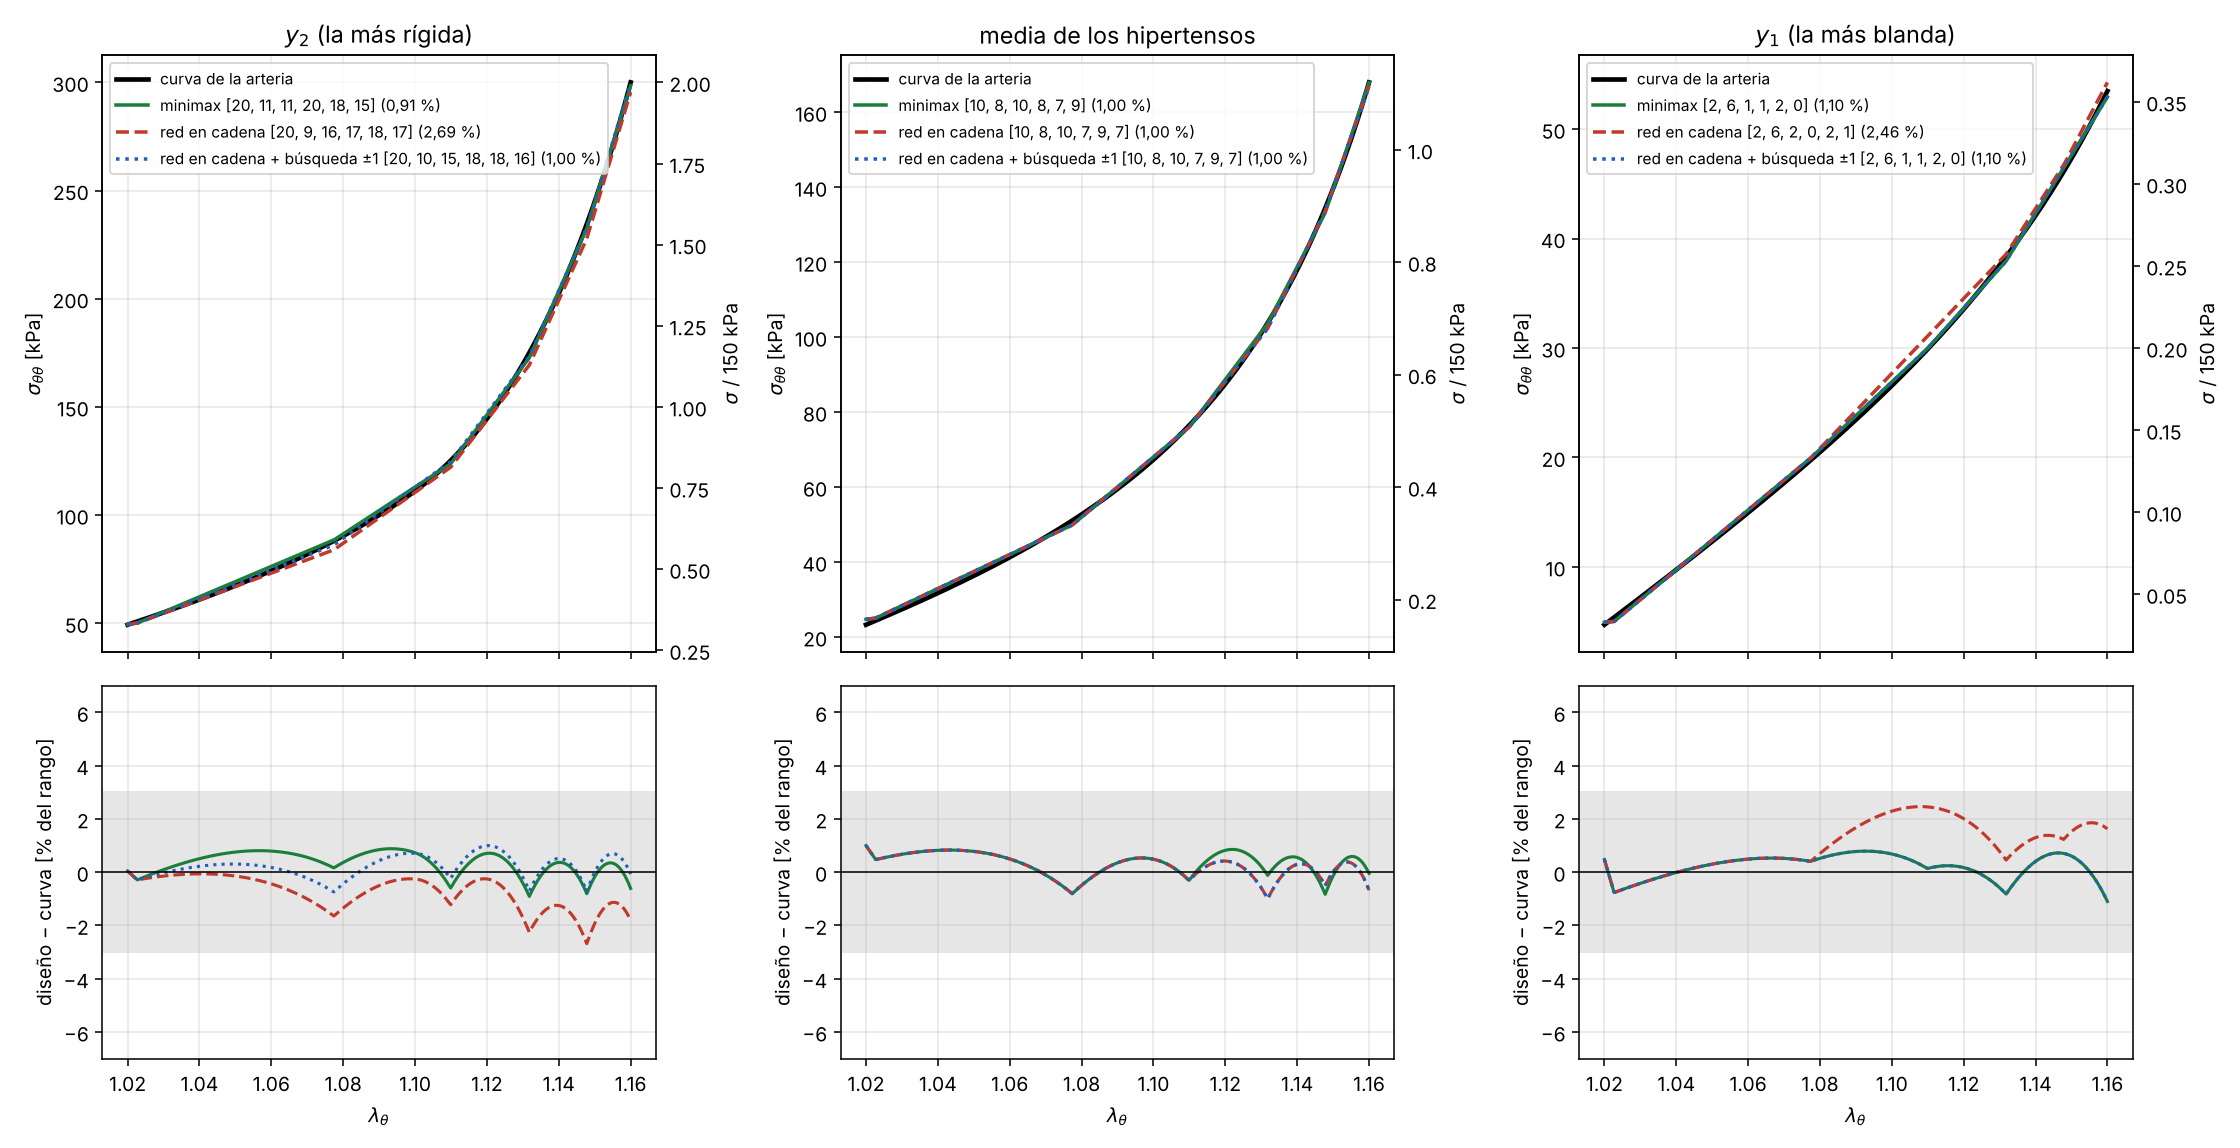
\includegraphics[width=\textwidth]{v58_limite_es.png}
\caption{6 materiales: la curva más rígida de la franja ($y_2$), la media de los hipertensos y la más blanda ($y_1$). Arriba: tensión (eje izquierdo en kPa, eje derecho relativo a 150\,kPa), con las láminas de cada material y el $e_{\max}$ de cada diseño; abajo: diseño $-$ curva en \% del rango (franja gris: meta de $\pm3$\,\%).}\label{fig:limite}\end{figure}
\begin{table}[H]\centering\small
\caption{Diseños de la Fig.~\ref{fig:limite} (6 materiales): láminas de cada material $c_j$ (reales en la primera fila de cada curva, enteras en las demás) y errores contra la curva original, $E_{\mathrm{rms}}$ y $e_{\max}$ [\% del rango].}\label{tab:limite}
\resizebox{\textwidth}{!}{\begin{tabular}{llcccccccc}\toprule
Curva & Método & $c_1$ & $c_2$ & $c_3$ & $c_4$ & $c_5$ & $c_6$ & $E_{\mathrm{rms}}$ & $e_{\max}$\\\midrule
$y_2$ & Mínimos cuadrados (reales) & 19,86 & 10,33 & 12,85 & 20,00 & 17,78 & 14,58 & 0,32 & 0,94\\
 & Minimax (MILP, referencia) & 20 & 11 & 11 & 20 & 18 & 15 & 0,54 & 0,91\\
 & Red en cadena & 20 & 9 & 16 & 17 & 18 & 17 & 0,98 & 2,69\\
 & Red en cadena + búsqueda $\pm1$ & 20 & 10 & 15 & 18 & 18 & 16 & 0,44 & 1,00\\
\addlinespace
Media HT & Mínimos cuadrados (reales) & 9,43 & 8,86 & 8,54 & 8,17 & 7,96 & 7,59 & 0,30 & 0,71\\
 & Minimax (MILP, referencia) & 10 & 8 & 10 & 8 & 7 & 9 & 0,54 & 1,00\\
 & Red en cadena & 10 & 8 & 10 & 7 & 9 & 7 & 0,50 & 1,00\\
 & Red en cadena + búsqueda $\pm1$ & 10 & 8 & 10 & 7 & 9 & 7 & 0,50 & 1,00\\
\addlinespace
$y_1$ & Mínimos cuadrados (reales) & 2,08 & 5,72 & 1,41 & 1,32 & 1,18 & 1,07 & 0,16 & 0,90\\
 & Minimax (MILP, referencia) & 2 & 6 & 1 & 1 & 2 & 0 & 0,49 & 1,10\\
 & Red en cadena & 2 & 6 & 2 & 0 & 2 & 1 & 1,36 & 2,46\\
 & Red en cadena + búsqueda $\pm1$ & 2 & 6 & 1 & 1 & 2 & 0 & 0,49 & 1,10\\
\bottomrule
\end{tabular}}
\end{table}

\paragraph{Tiempo.} El minimax tarda unos 50 a 65\,ms por curva y no se acelera en lote, porque resuelve un problema por curva. La red, en lote, tarda 0,3\,ms por curva (0,2 con 5 materiales), y con la búsqueda de $\pm1$, 2,0\,ms (0,7 con 5): de 30 a 200 veces menos. Para una sola curva el tiempo lo fija la llamada a la biblioteca de redes (unos 0,3\,s con TensorFlow), no el cálculo. La ventaja de la red no es solo el tiempo: da el diseño sin resolver ninguna optimización, con la misma operación para cualquier curva del dominio de validez.

\subsection{Validación externa: mediciones de otros autores}\label{sec:externa}
Para comprobar que el método no depende de la arteria con que se construyó, se aplicó a curvas $\sigma_{\theta\theta}(\lambda_\theta)$ de tres estudios independientes, con otras leyes constitutivas, otras arterias, capas aisladas y mediciones in vivo. \textbf{No se cambió nada}: los mismos nudos y pendientes (Tabla~\ref{tab:bases}), la misma red, el mismo dominio de validez y el mismo minimax. Ninguna de estas leyes está en el entrenamiento de la red.

\paragraph{Curvas y leyes constitutivas.} Cada curva se recalcula con la ley constitutiva y los parámetros que publicaron sus autores. La ley se usa tal cual porque es la que esos autores ajustaron a sus mediciones: es la que fija la forma de la curva y, con ella, lo que el injerto tiene que reproducir.
\begin{itemize}
\item \textbf{Sommer y Holzapfel}~\cite{sommer}: carótidas común (CCA) e interna (ICA) de 11 donantes (77,6 años en promedio), ensayadas por extensión--inflado como tubos de pared intacta, de adventicia y de media--íntima~\cite{sommer2010}. Los autores ajustaron a cada espécimen la ley de Holzapfel, Gasser y Ogden~\cite{holzapfel} con dispersión de fibras,
\begin{gather*}
\Psi=\tfrac{\mu}{2}(I_1-3)+\tfrac{k_1}{k_2}\bigl(e^{Q}-1\bigr),\\
Q=k_2\bigl[(1-\rho)(I_1-3)^2+\rho\,(I_4-1)^2\bigr],\qquad I_4=\lambda_\theta^2\cos^2\varphi+\lambda_z^2\sin^2\varphi,
\end{gather*}
donde $\mu$ es la rigidez de la matriz (elastina), $k_1$ y $k_2$ la rigidez y el endurecimiento del colágeno, $\varphi$ el ángulo de las fibras y $\rho$ su grado de alineación; las fibras no trabajan en compresión ($I_4<1$). Los cinco parámetros de cada espécimen están en sus Tablas~1 y~2. Se usa $\sigma_{\theta\theta}-\sigma_{rr}$ con $\lambda_z=1{,}10$, el estiramiento axial in vivo que adoptan los autores~\cite{sommer2010}.
\item \textbf{Liu et al.}~\cite{liu}: 12 carótidas humanas con placa, caracterizadas in vivo con resonancia magnética cine y multicontraste. Los autores identificaron para cada paciente un Mooney--Rivlin modificado en tracción uniaxial,
\begin{equation*}
\sigma=2\lambda\bigl(\lambda-\lambda^{-2}\bigr)\Bigl(c_1+D_1D_2\,e^{D_2(\lambda^2+2/\lambda-3)}\Bigr),\qquad D_2=2,
\end{equation*}
con $c_1$ y $D_1$ de su Tabla~1. Publican también la contracción circunferencial $S$ entre el estado sin carga y la diástole y los perímetros diastólico y sistólico, que dan la ventana medida.
\item \textbf{Kamenskiy et al.}~\cite{kamenskiy}: 16 pacientes, carótidas común, externa (ECA) e interna medidas in vivo por ultrasonido a lo largo del ciclo cardíaco (48 curvas). Por cada arteria publican la tensión y el módulo tangente en diástole y en sístole y los diámetros. La ley más simple que reproduce esos datos con forma de J es la exponencial, $\sigma(\varepsilon)=\sigma_d+\alpha\bigl(e^{\beta\varepsilon}-1\bigr)$ en $\varepsilon\in[0,\varepsilon_s]$: con $\sigma(\varepsilon_s)=\sigma_s$ exacta y $\beta$ que reproduce las dos pendientes. En las 48 arterias la pendiente sistólica supera a la diastólica: todas son J.
\end{itemize}
Se excluyó la carótida de conejo de Holzapfel et al.~\cite{holzapfel}: como capas aisladas, con la geometría del conejo, a esas presiones da tensiones de 900 a 3300\,kPa, lejos de cualquier carótida humana.

\paragraph{Un solo escalamiento: la ventana de presión.} Cada curva vive en su propio rango de $\lambda$ y se lleva a $[1{,}02;\,1{,}16]$ con un cambio afín de $\lambda$: el estiramiento a la presión baja va a 1,02 y el de la presión alta a 1,16. \textbf{La tensión no se toca}: cada curva conserva las suyas, sin fijar de antemano su valor en los extremos. El cambio de $\lambda$ equivale a lo que el injerto real permite: un preestiramiento (corrimiento de los nudos, el $\delta$ de la Sección~\ref{sec:aplicacion}) y la elección del radio de referencia. La ventana sale de la presión:
\begin{itemize}
\item \textbf{M (in vivo, medida):} Liu y Kamenskiy, entre la diástole y la sístole de cada paciente.
\item \textbf{P (ex vivo, calculada):} Sommer y Holzapfel, entre 60 y 200\,mmHg, la misma ventana de presión del nivel tubo (Sección~\ref{sec:aplicacion}). El estiramiento a cada presión sale del equilibrio de pared delgada que usan Sommer et al.~\cite{sommer2010} (sus ecs.~1 y~2),
\begin{equation*}
\sigma_{\theta\theta}=p\Bigl(\frac{r}{h}-1\Bigr),\qquad r=R\,\lambda_\theta,\qquad R^2-(R-H)^2=\bigl[r^2-(r-h)^2\bigr]\lambda_z,
\end{equation*}
con el radio externo $R$ y el espesor $H$ sin carga medios de cada arteria y capa (su Tabla~2): pared intacta 4,15 y 1,17\,mm (CCA) y 2,67 y 0,86\,mm (ICA); adventicia 4,00 y 0,47 y 2,51 y 0,33\,mm; media--íntima 3,61 y 0,70 y 2,15 y 0,53\,mm. Tres adventicias (CCA II\,l y VIII\,r, ICA VIII\,r) ya soportan sin carga más de 60\,mmHg y no tienen ventana: se excluyen.
\end{itemize}
Con 60\,mmHg las curvas ex vivo arrancan entre 21 y 92\,kPa y con 200\,mmHg llegan a entre 76 y 325\,kPa; las in vivo recorren de 13 a 389\,kPa. En total, 98 curvas: 38 de Sommer y Holzapfel, 12 de Liu y 48 de Kamenskiy (Fig.~\ref{fig:ext}).

\begin{figure}[H]\centering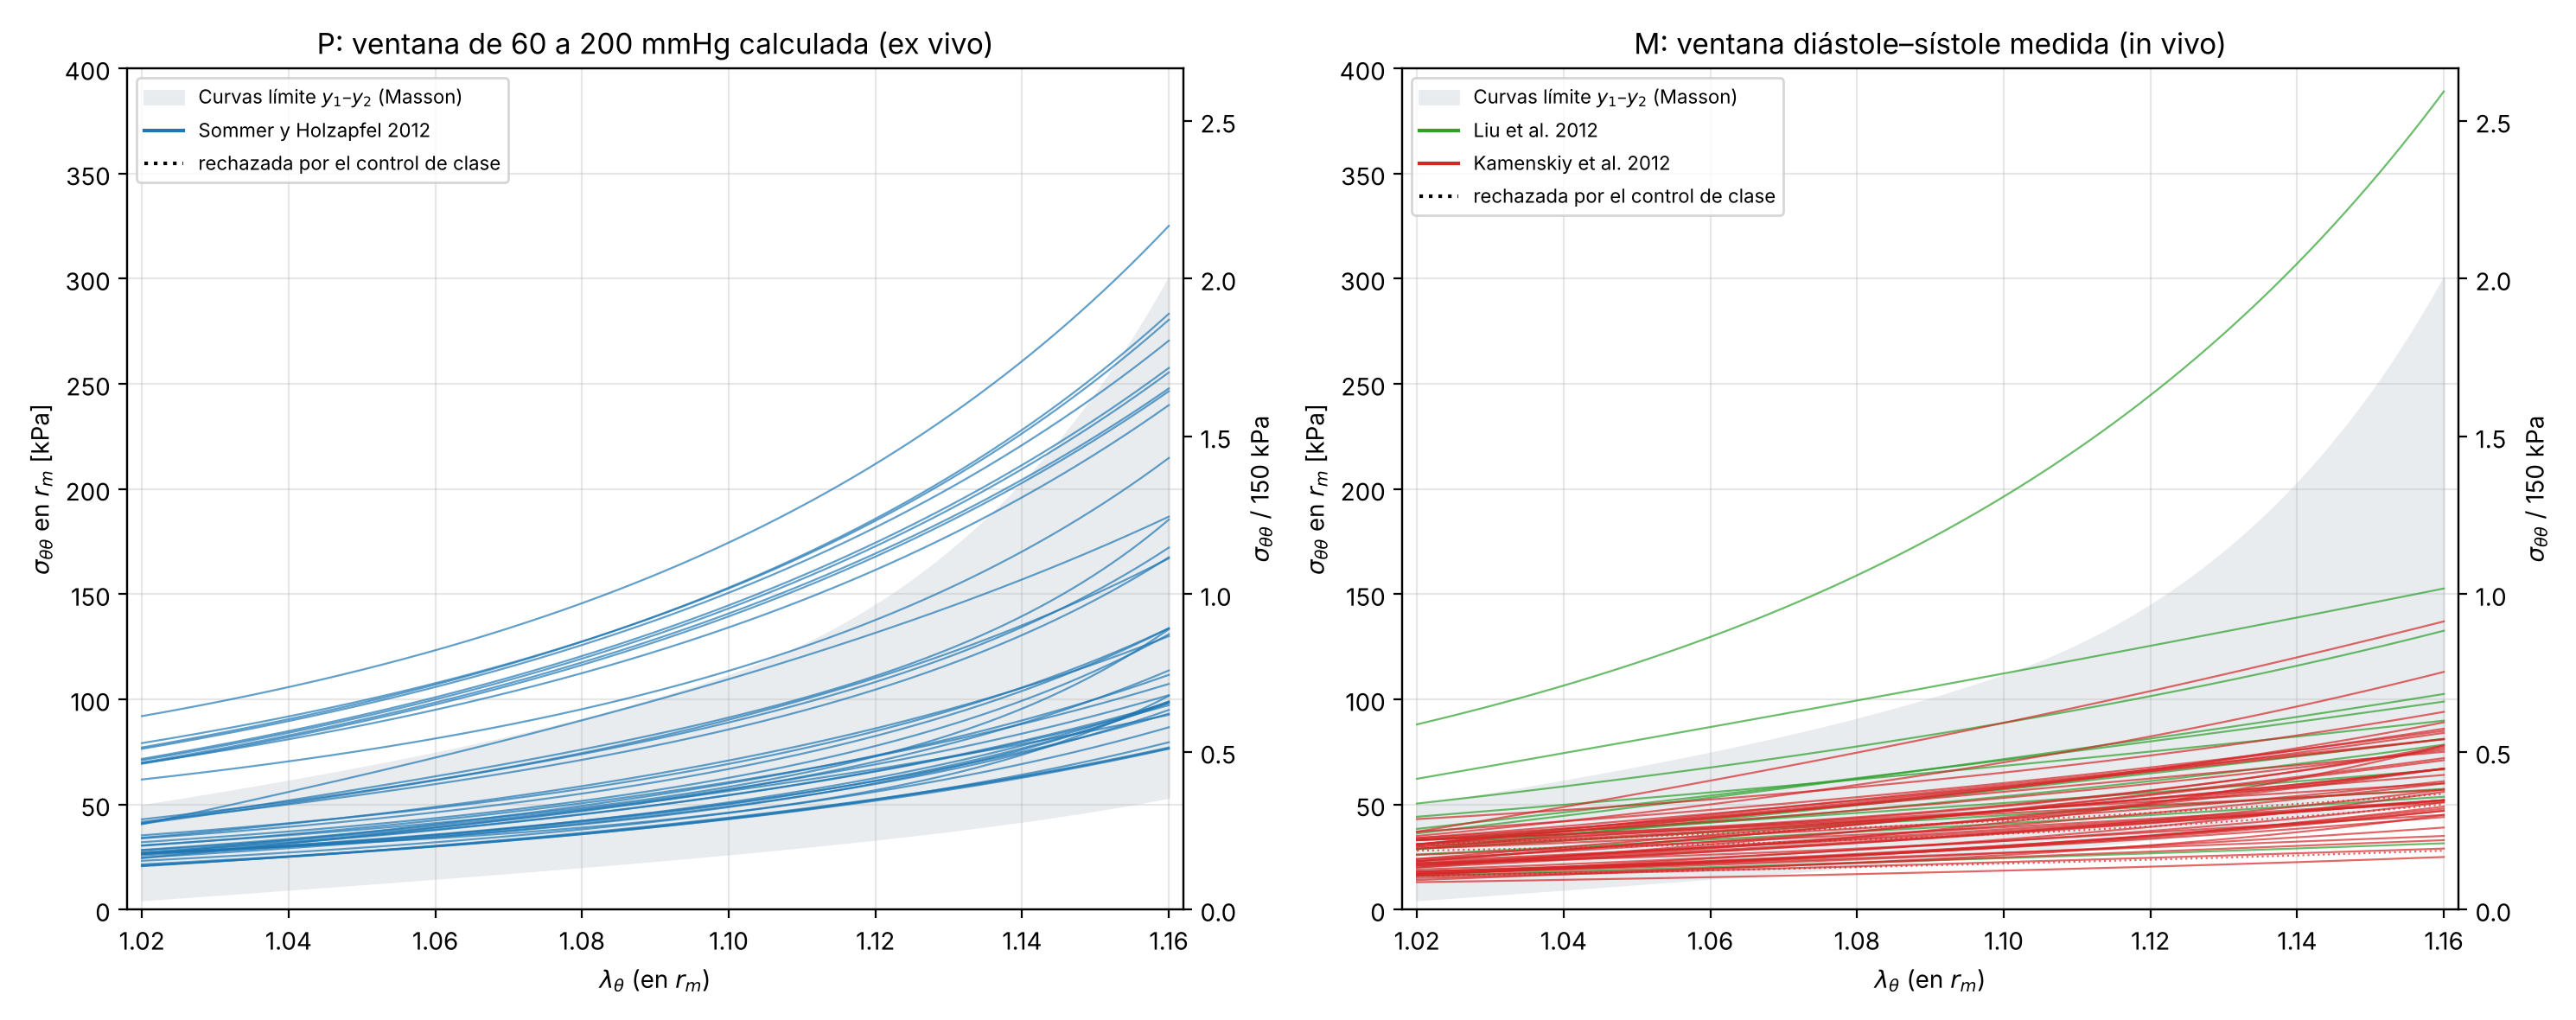
\includegraphics[width=\textwidth]{v54_curvas_externas_es.png}
\caption{Las 98 curvas externas en el dominio de diseño, con las escalas de la Fig.~\ref{fig:sigma}: eje izquierdo en kPa, eje derecho relativo a 150\,kPa (aquí hasta 400\,kPa, porque una curva de Liu et al.\ llega a 389\,kPa). Las dos con el mismo escalamiento: cada curva entre su presión baja y su presión alta, con sus propias tensiones. Izquierda: ventana de 60 a 200\,mmHg calculada con la geometría de cada arteria y capa (Sommer y Holzapfel); derecha: ventana diástole--sístole medida in vivo (Liu, Kamenskiy). Franja gris: curvas límite $y_1$--$y_2$ de la población de Masson, el dominio de validez del método; solo las curvas que quedan enteras dentro de ella forman la validación externa. Punteadas: rechazadas por el control de clase.}\label{fig:ext}\end{figure}

\paragraph{Curvas dentro del dominio de validez.} De las 98 curvas, el control de clase rechazó 3: las tres ventanas in vivo más cortas de Kamenskiy (ECA de los pacientes 11 y 15 e ICA del 15, con $\varepsilon_s\le3$\,\%). De las 95 restantes, 63 quedan enteras dentro de $y_1$--$y_2$ y forman la validación externa: las 28 paredes intactas y media--íntimas de Sommer y Holzapfel, 8 curvas de Liu y 27 de Kamenskiy. Las 32 que salen de la franja no se usan, porque la red no puede asegurar en ellas la meta: las 10 adventicias aisladas, que a 200\,mmHg superan a $y_2$; 4 de Liu (P11 llega a 389\,kPa); y 18 de Kamenskiy.

\paragraph{Resultados.} La Tabla~\ref{tab:extres} resume, por estudio, las 63 curvas; la Fig.~\ref{fig:emax} muestra el $e_{\max}$ de cada curva, y las Tablas~\ref{tab:ext6} y~\ref{tab:ext5} (Anexo~\ref{sec:tablas}), las láminas y los errores de cada una.

\begin{table}[H]\centering\small
\caption{Validación externa: las 63 curvas dentro de $y_1$--$y_2$. Curvas que cumplen la meta de 3\,\% con láminas enteras y peor $e_{\max}$ [\%] de cada método.}\label{tab:extres}
\resizebox{\textwidth}{!}{\begin{tabular}{lc|ccc|ccc}\toprule
 & & \multicolumn{3}{c|}{6 materiales} & \multicolumn{3}{c}{5 materiales}\\
Estudio & Curvas & Minimax & Red & Red $+\pm1$ & Minimax & Red & Red $+\pm1$\\\midrule
Sommer y Holzapfel~\cite{sommer} (pared y media--íntima) & 28 & 28 · 2,52 & 28 · 2,64 & 28 · 2,64 & 28 · 2,76 & 27 · 3,31 & 27 · 3,31\\
Liu et al.~\cite{liu} & 8 & 5 · 3,74 & 4 · 5,64 & 5 · 5,64 & 5 · 3,91 & 4 · 3,91 & 5 · 3,91\\
Kamenskiy et al.~\cite{kamenskiy} & 27 & 24 · 5,71 & 14 · 9,44 & 17 · 6,16 & 21 · 5,98 & 12 · 7,55 & 16 · 5,98\\\midrule
Total & 63 & 57 & 46 & 50 & 54 & 43 & 48\\\bottomrule
\end{tabular}}
\end{table}

\begin{figure}[H]\centering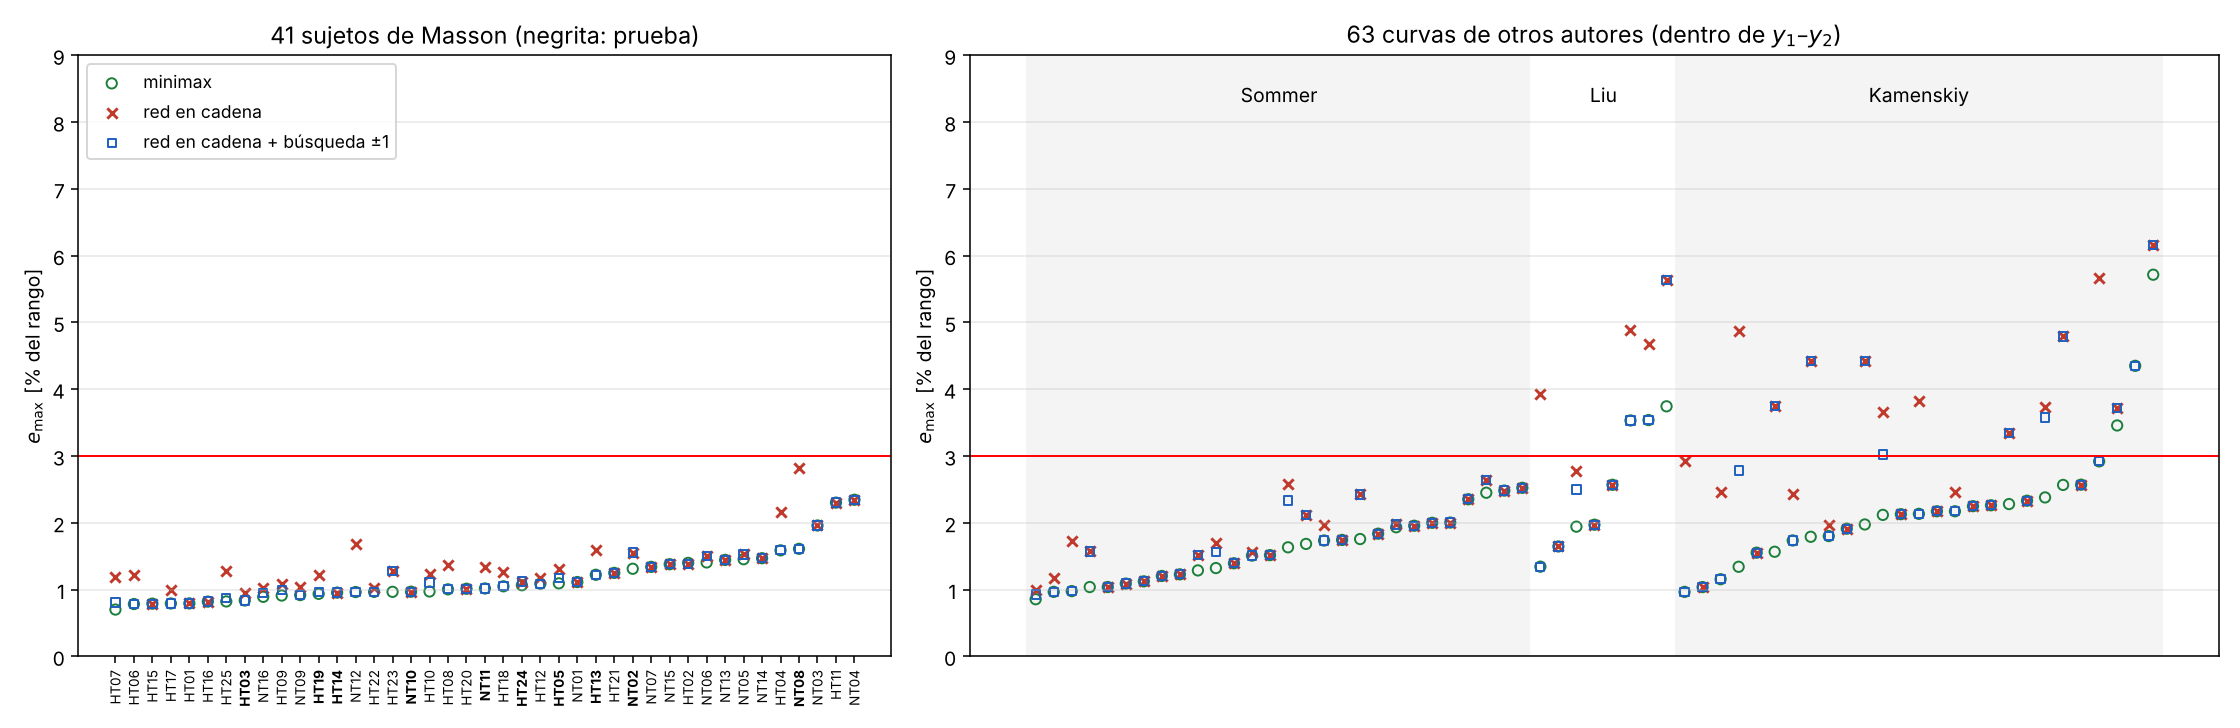
\includegraphics[width=\textwidth]{v58_emax_es.png}
\caption{Peor error de cada curva con láminas enteras, 6 materiales: minimax (círculos), red en cadena (cruces) y red en cadena con búsqueda de $\pm1$ (cuadrados). Izquierda: los 41 sujetos de Masson, ordenados por el error del minimax (en negrita, los de prueba). Derecha: las 63 curvas externas dentro de $y_1$--$y_2$, por estudio. Línea roja: meta de 3\,\%.}\label{fig:emax}\end{figure}

\begin{enumerate}[label=(\roman*)]
\item \textbf{La base alcanza.} Con mínimos cuadrados, las 63 curvas cumplen la meta: peor error de 1,28\,\% con 6 materiales y 1,84\,\% con 5.
\item \textbf{El techo de las láminas enteras.} El minimax cumple en 57 de las 63 (6 materiales) y en 54 (5). Las que no cumplen ni con el minimax son curvas in vivo de poco recorrido de tensión (de 26 a 36\,kPa con 6 materiales, contra una mediana de 56\,kPa en las 63), casi rectas, en las que el primer material lleva casi todo el diseño: una lámina de más o de menos mueve la curva más de lo que permite la meta, que en ellas es de 1\,kPa o menos. El peor error del minimax en esas curvas es de 1,0 a 1,7\,kPa. Con cantidades reales cumplen todas: el límite lo pone la división en 20 láminas por material, no la base ni la red.
\item \textbf{La red.} Sola, cumple en 46 de 63 (6 materiales) y 43 (5); con la búsqueda de $\pm1$, en 50 y 48. En las 28 curvas de Sommer y Holzapfel, con 6 materiales, la red cumple en todas ya sin la búsqueda, como el minimax; en Liu, con la búsqueda, en las mismas 5 que el minimax. Donde queda por debajo del minimax ---7 curvas in vivo de Kamenskiy con 6 materiales--- la red se equivocó en más de una lámina, y una revisión de $\pm1$ no alcanza. Da exactamente el diseño del minimax en 8 curvas (18 con la búsqueda).
\end{enumerate}

\paragraph{Resultado global.} Sumando los 41 sujetos y las 63 curvas externas (6 materiales), el minimax cumple en 98 de 104: es el techo, porque ningún diseño entero cumple en las otras 6. La red en cadena con búsqueda de $\pm1$ cumple en 91, el 93\,\% de lo alcanzable con láminas enteras, sin resolver ninguna optimización; sola, en 87. Separado por conjunto: 31 de 31 sujetos de entrenamiento, 10 de 10 de prueba y 50 de 63 curvas externas.

\begin{caja}{Conclusión del primer nivel}
Con materiales tipo fibra y una base elegida una vez, la curva tensión--estiramiento de las 41 carótidas se reproduce con láminas enteras dentro de la meta (6 materiales, a lo sumo 20 láminas por material). El minimax da el mejor diseño entero que existe y es la referencia. Una sola red neuronal, la red en cadena con salida ordinal, entrenada dentro de la franja $y_1$--$y_2$ ---su dominio de validez---, da directamente las láminas enteras en una evaluación: con una búsqueda de $\pm1$ lámina cumple en los 10 sujetos de prueba y en 50 de 63 curvas de otros tres estudios, con otras leyes constitutivas, y llega a 91 de los 98 casos que admiten un diseño entero dentro de la meta. Fuera de la franja la red no se usa.
\end{caja}

%=====================================================================
\section{Aplicación: la curva presión--diámetro y el tubo de pared gruesa}\label{sec:aplicacion}
\subsection{De la tensión a la presión}
Un injerto se implanta como tubo, y lo que debe coincidir con la arteria es su diámetro a cada presión. Para pasar de la tensión a la presión hacen falta la geometría y una hipótesis sobre la pared. La configuración libre de tensiones de la arteria es un sector anular abierto de semiángulo $\Theta_0$ y radio $R_m$ en el borde media--adventicia, que representa las tensiones residuales (Fig.~\ref{fig:estados}). Un punto de radio $R$ en el sector pasa al radio $r$ en la arteria cerrada; su estiramiento y la conservación del volumen dan~\cite{masson}
\begin{equation}\label{eq:cinem}
\lambda_\theta=\frac{\pi r}{\Theta_0R},\qquad \Theta_0\,(R_m^2-R^2)=\pi\lambda_z\,(r_m^2-r^2).
\end{equation}
El equilibrio radial integrado sobre el espesor da la presión que soporta la pared íntima--media~\cite{masson,humphrey}:
\begin{equation}\label{eq:equil}
P=P_i-P_a=\int_{r_i}^{r_m}\frac{\sigma_{\theta\theta}-\sigma_{rr}}{r}\,dr,
\end{equation}
con $P_i$ la presión de la sangre y $P_a$ la que ejercen la adventicia y el tejido que rodea a la arteria. Como $P_a$ depende del sitio, el diseño se plantea sobre $P$, la presión que soporta la pared, que es la que el injerto debe soportar con la misma deformación. El espesor íntima--media $h$ se toma de la mediana de referencia por edad y sexo medida con ecotracking~\cite{engelen13} (0,43 a 0,68\,mm), porque Masson et al.\ no publican el de cada sujeto, y $r_i=r_m-h$.

\begin{figure}[H]\centering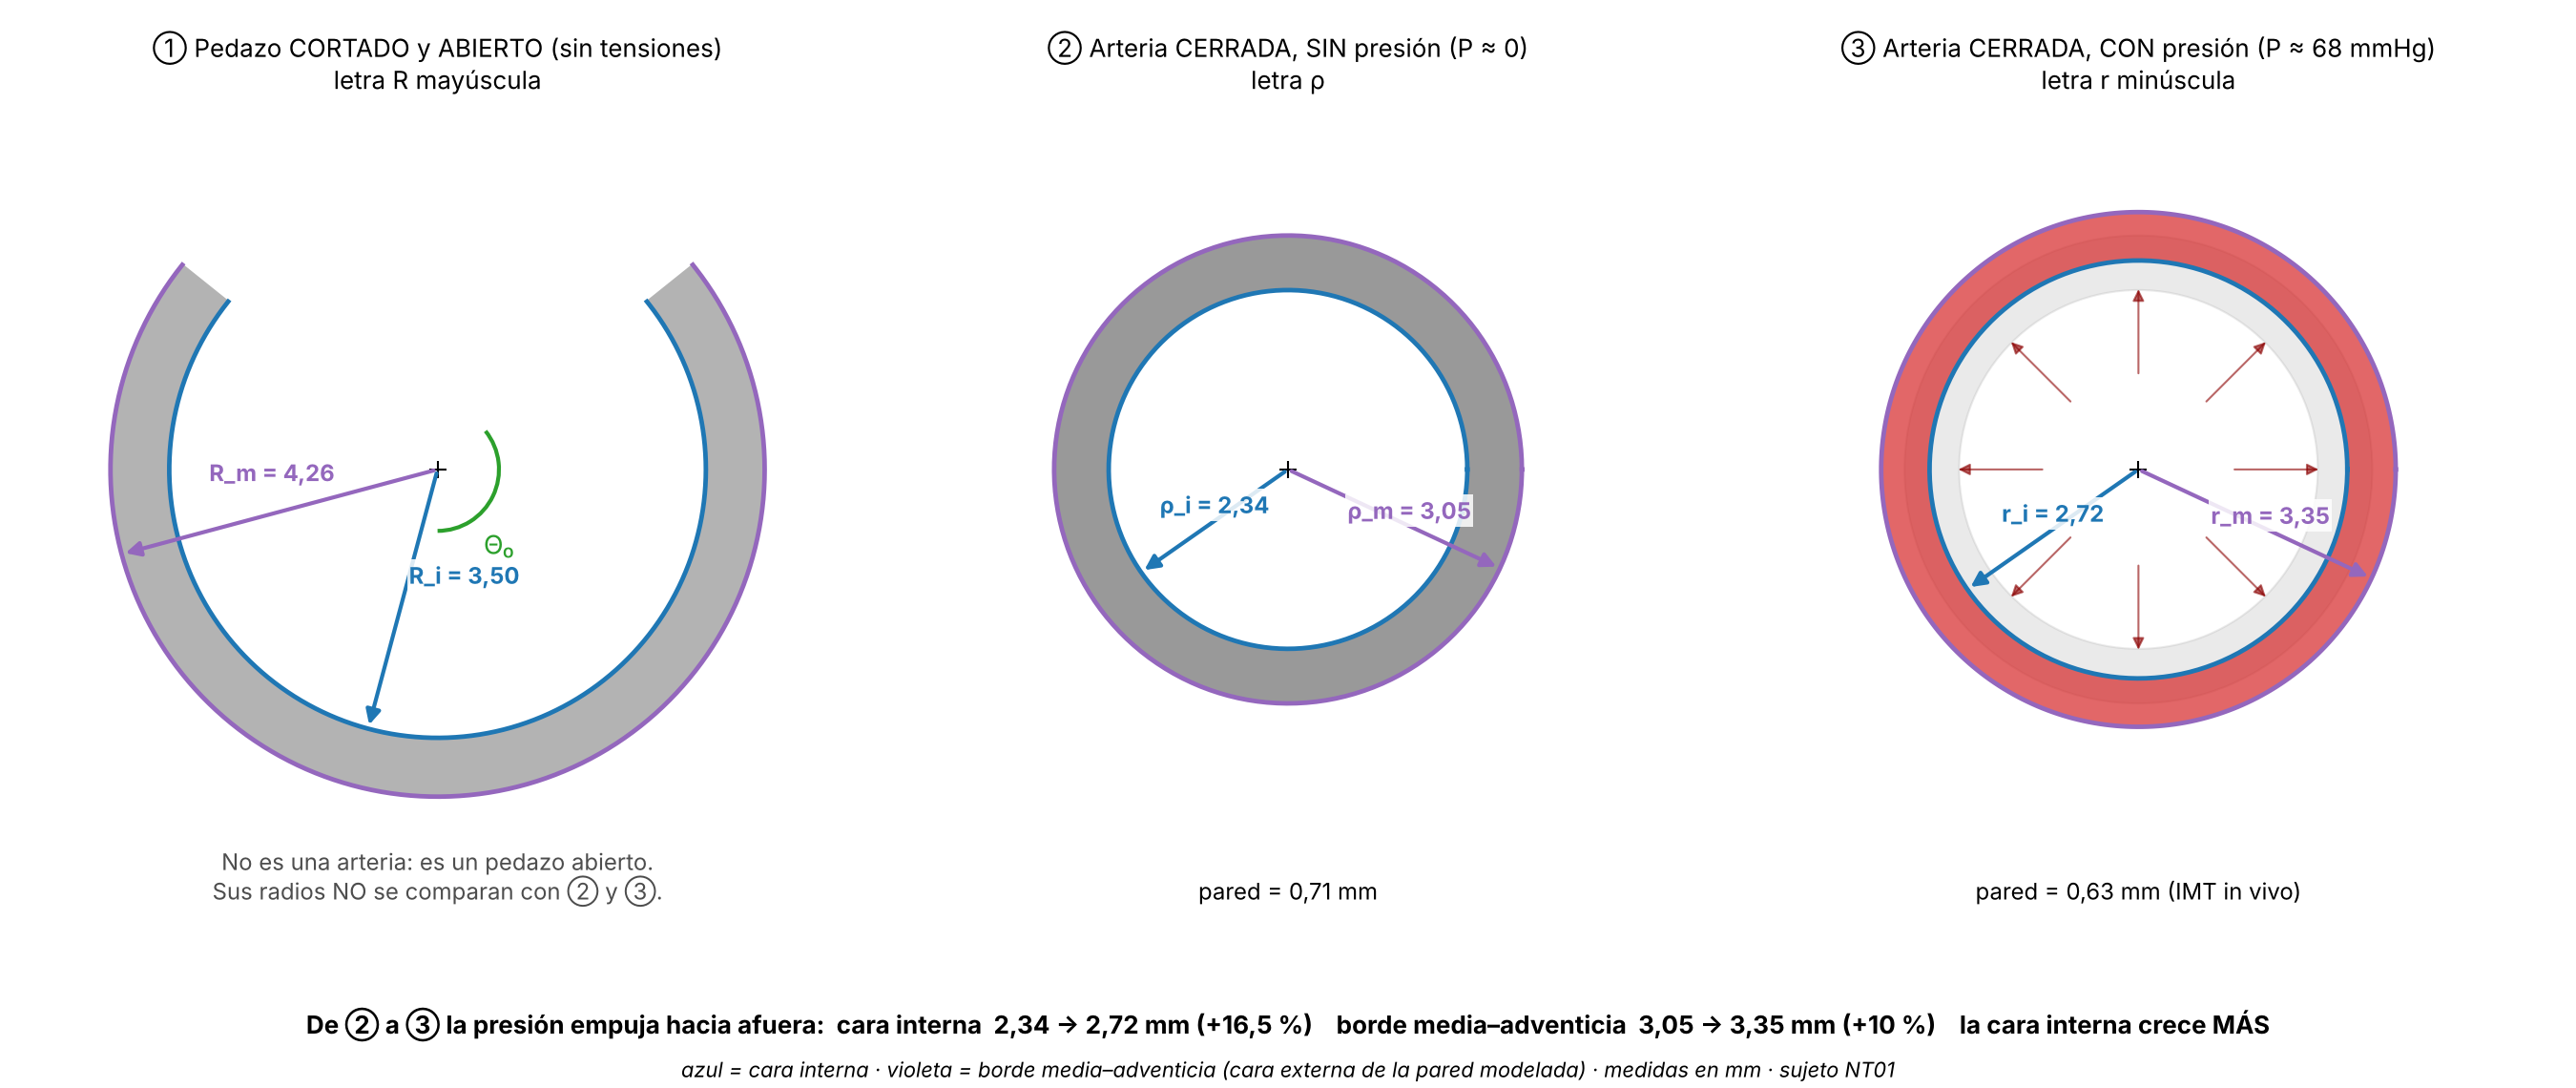
\includegraphics[width=\textwidth]{d10_tres_estados.png}
\caption{Sujeto NT01 en sus tres estados: (1) sector abierto sin tensiones, (2) arteria cerrada sin presión, (3) arteria con presión. De (2) a (3) la cara interna crece 16,5\,\% y el borde media--adventicia 10\,\%.}\label{fig:estados}\end{figure}

\paragraph{Ventana de presión.} Lo que define si un estado es fisiológico es la presión, no el estiramiento: en $\lambda_\theta=1{,}16$ el sujeto más rígido soporta unos 400\,mmHg y uno blando joven, unos 70. Por eso, en este nivel, todos los sujetos se evalúan en la misma ventana, $P$ de 60 a 200\,mmHg (8,0 a 26,7\,kPa) en 141 valores, que cubre con margen las presiones medias medidas (64/116\,mmHg en NT y 73/127\,mmHg en HT~\cite{masson}). La curva objetivo es el estiramiento del borde media--adventicia, $\lambda(P_k)$, proporcional al diámetro (Fig.~\ref{fig:presion}): los sujetos rígidos llegan a 200\,mmHg con $\lambda$ entre 1,12 y 1,15, los blandos con $\lambda$ entre 1,20 y 1,23.

\begin{figure}[H]\centering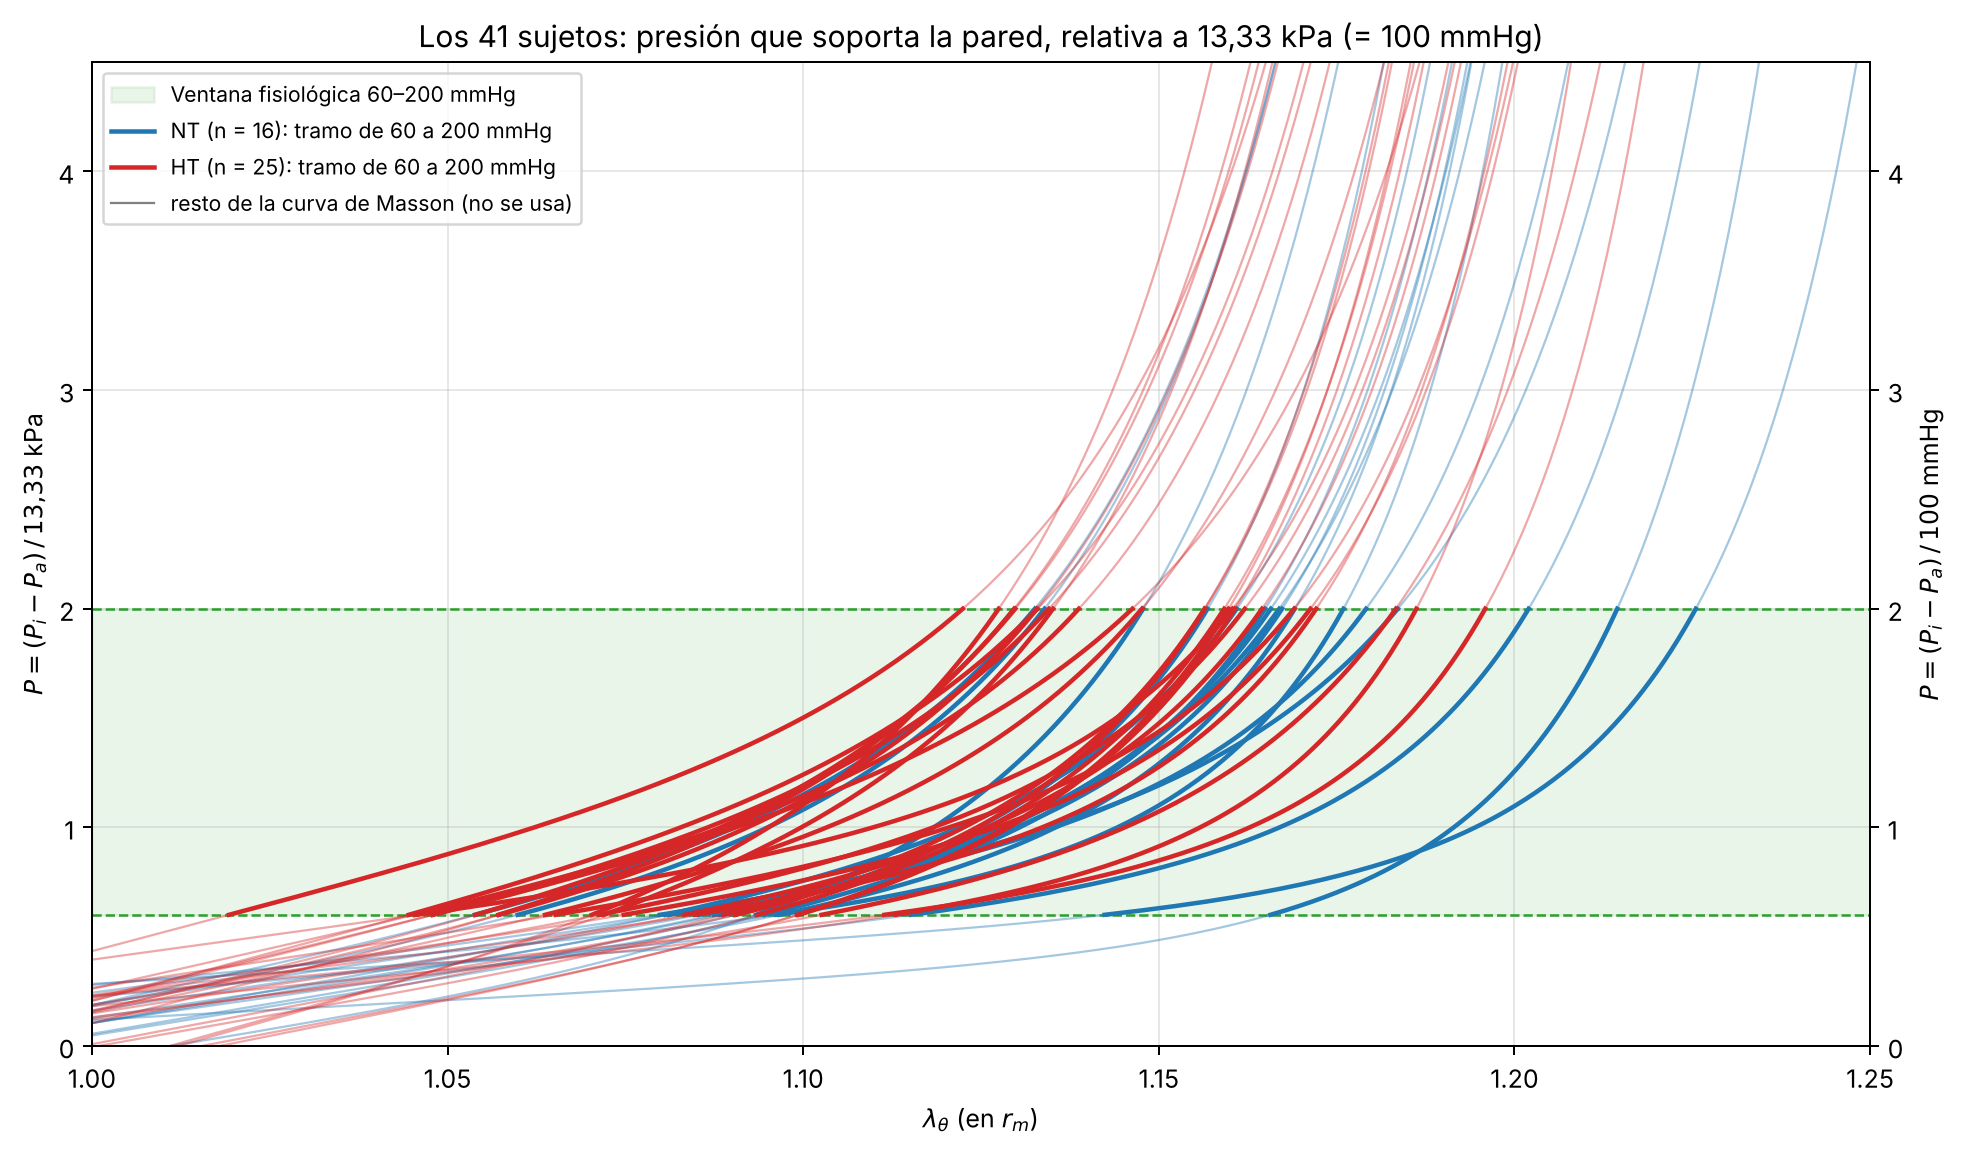
\includegraphics[width=0.85\textwidth]{f_sujetos_relativa.png}
\caption{Los 41 sujetos: presión que soporta la pared, en función del estiramiento del borde media--adventicia, en forma relativa: $P=(P_i-P_a)/13{,}33$\,kPa a la izquierda y $P=(P_i-P_a)/100$\,mmHg a la derecha. Como $13{,}33$\,kPa $=100$\,mmHg, las dos escalas coinciden; la ventana de 60 a 200\,mmHg va de 0,6 a 2. Trazo grueso: tramo de 60 a 200\,mmHg, que es la curva objetivo.}\label{fig:presion}\end{figure}

\subsection{El problema: la pared de la carótida es gruesa}
Si la pared es delgada frente al radio, todas sus fibras se estiran lo mismo y el equilibrio de medio tubo da la ley de Laplace, $P=\sum_j\sigma_jh_j/r$~\cite{fung}: la presión es lineal en los espesores de las capas y todo el método del primer nivel pasaría tal cual al tubo. La carótida, sin embargo, tiene una pared de alrededor de un 20\,\% del radio. Al inflarse, sus fibras internas se estiran más que las externas (Fig.~\ref{fig:fibra}), porque la pared es incompresible: cada fibra conserva el área que tiene por dentro.

\begin{figure}[H]\centering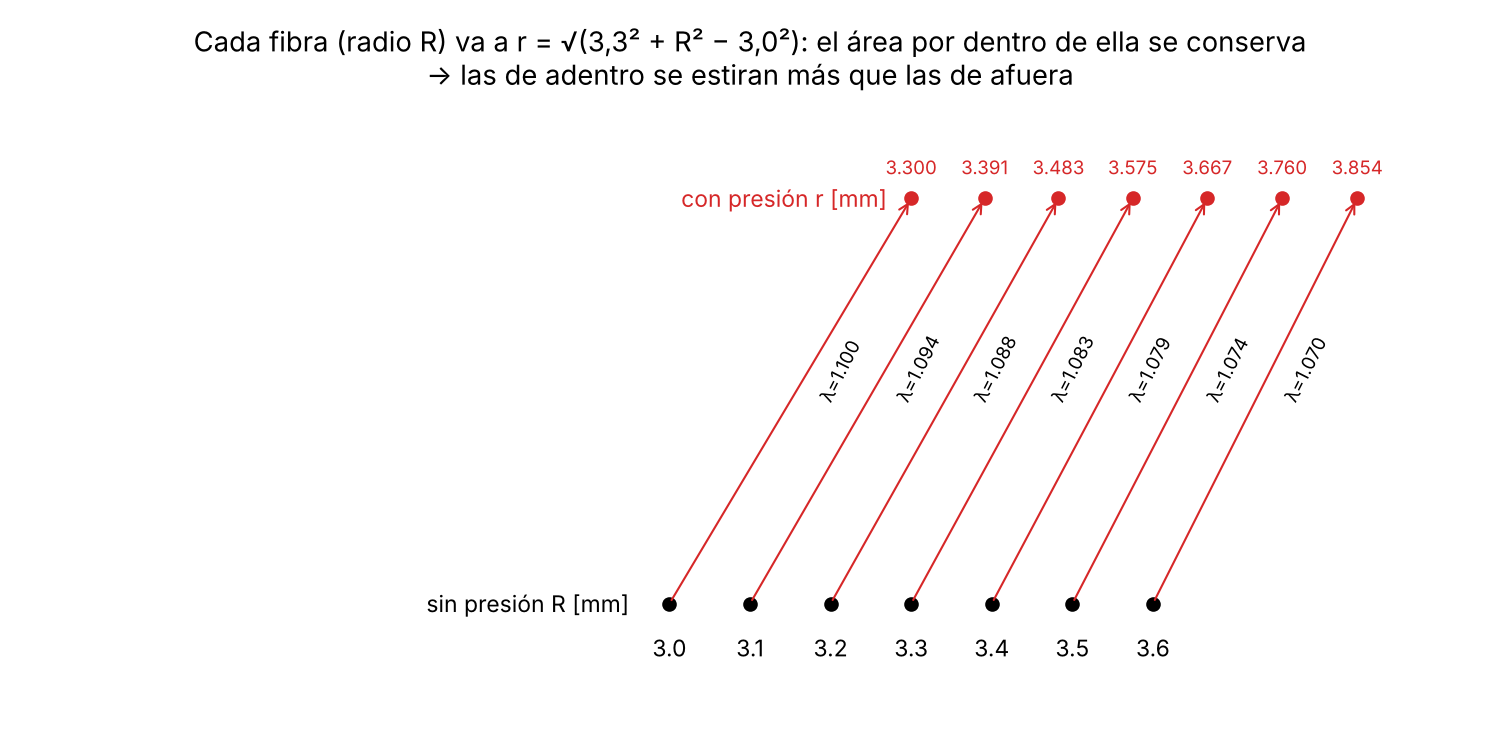
\includegraphics[width=0.78\textwidth]{d6_cada_fibra.png}
\caption{Tubo de 3,0 a 3,6\,mm inflado hasta una cara interna de 3,3\,mm: cada fibra conserva el área que tiene por dentro; la cara interna se estira 10\,\% y la externa 7\,\%.}\label{fig:fibra}\end{figure}

Con los materiales del primer nivel, que no tiran hasta su nudo, esa diferencia de pocos centésimos decide si una capa trabaja: un material de nudo 1,08 tira en la cara interna del tubo de la Fig.~\ref{fig:fibra} ($\lambda=1{,}10$) y no en la externa ($\lambda=1{,}07$). Por eso la presión se calcula sumando el aporte de cada capa delgada, cada una con su propio estiramiento:
\begin{equation}\label{eq:pgruesa}
P=\sum_{j=1}^{N}\int_{\text{capa }j}\frac{\sigma_j\bigl(\lambda(r)\bigr)}{r}\,dr .
\end{equation}
Si la pared es muy delgada, \eqref{eq:pgruesa} se reduce a Laplace. En la carótida no: además, las capas se influyen entre sí, porque si crece una capa interna las de afuera quedan a radios mayores, se estiran menos y aportan menos. La presión deja de ser lineal en los espesores. El Anexo~\ref{sec:ejemplo} lo muestra con un ejemplo que se puede seguir a mano.

\subsection{La consecuencia: un diseño de pared delgada falla al fabricarse}
Se diseñó cada sujeto con tres hipótesis ---Laplace, la ley de pared delgada de Urquiza~\cite{urquiza}, que usa el radio medio deformado, y pared gruesa \eqref{eq:pgruesa}--- y cada diseño se evaluó en el tubo que realmente se fabrica, que es de pared gruesa (Tabla~\ref{tab:laplace}, Fig.~\ref{fig:laplace}). Diseñado con Laplace, el injerto parece perfecto en su propio modelo, pero al fabricarlo \textbf{ningún sujeto cumple la meta}; diseñado en pared gruesa, \textbf{cumplen los 41}. Corregir el radio, como hace Urquiza, no alcanza: el problema no es el radio, sino que cada capa se estira distinto y empieza a tirar en otro momento. \textbf{El diseño del tubo debe hacerse en pared gruesa.} Los detalles de esta comparación están en el Anexo~\ref{sec:calculo}.

\begin{table}[H]\centering\small
\caption{Hipótesis con que se \emph{diseña} el injerto; todos los diseños se \emph{evalúan} en el tubo de pared gruesa, que es el que se fabrica. En cada celda, para los 41 sujetos: cuántos cumplen $e_{\max}\le3$\,\%, la mediana de $e_{\max}$ y el peor $e_{\max}$. Comparación hecha con espesores reales y con un juego de nudos y módulos propio (Anexo~\ref{sec:calculo}).}\label{tab:laplace}
\begin{tabular}{lcc}\toprule
Hipótesis de diseño & 5 materiales & 6 materiales\\\midrule
Laplace & 0/41 · 13,6\,\% · 22,7\,\% & 0/41 · 14,8\,\% · 32,5\,\%\\
Urquiza (radio medio deformado) & 0/41 · 13,7\,\% · 24,5\,\% & 0/41 · 15,4\,\% · 34,4\,\%\\
Pared gruesa & 41/41 · 0,96\,\% · 2,97\,\% & 41/41 · 0,72\,\% · 2,10\,\%\\\bottomrule
\end{tabular}
\end{table}
\begin{figure}[H]\centering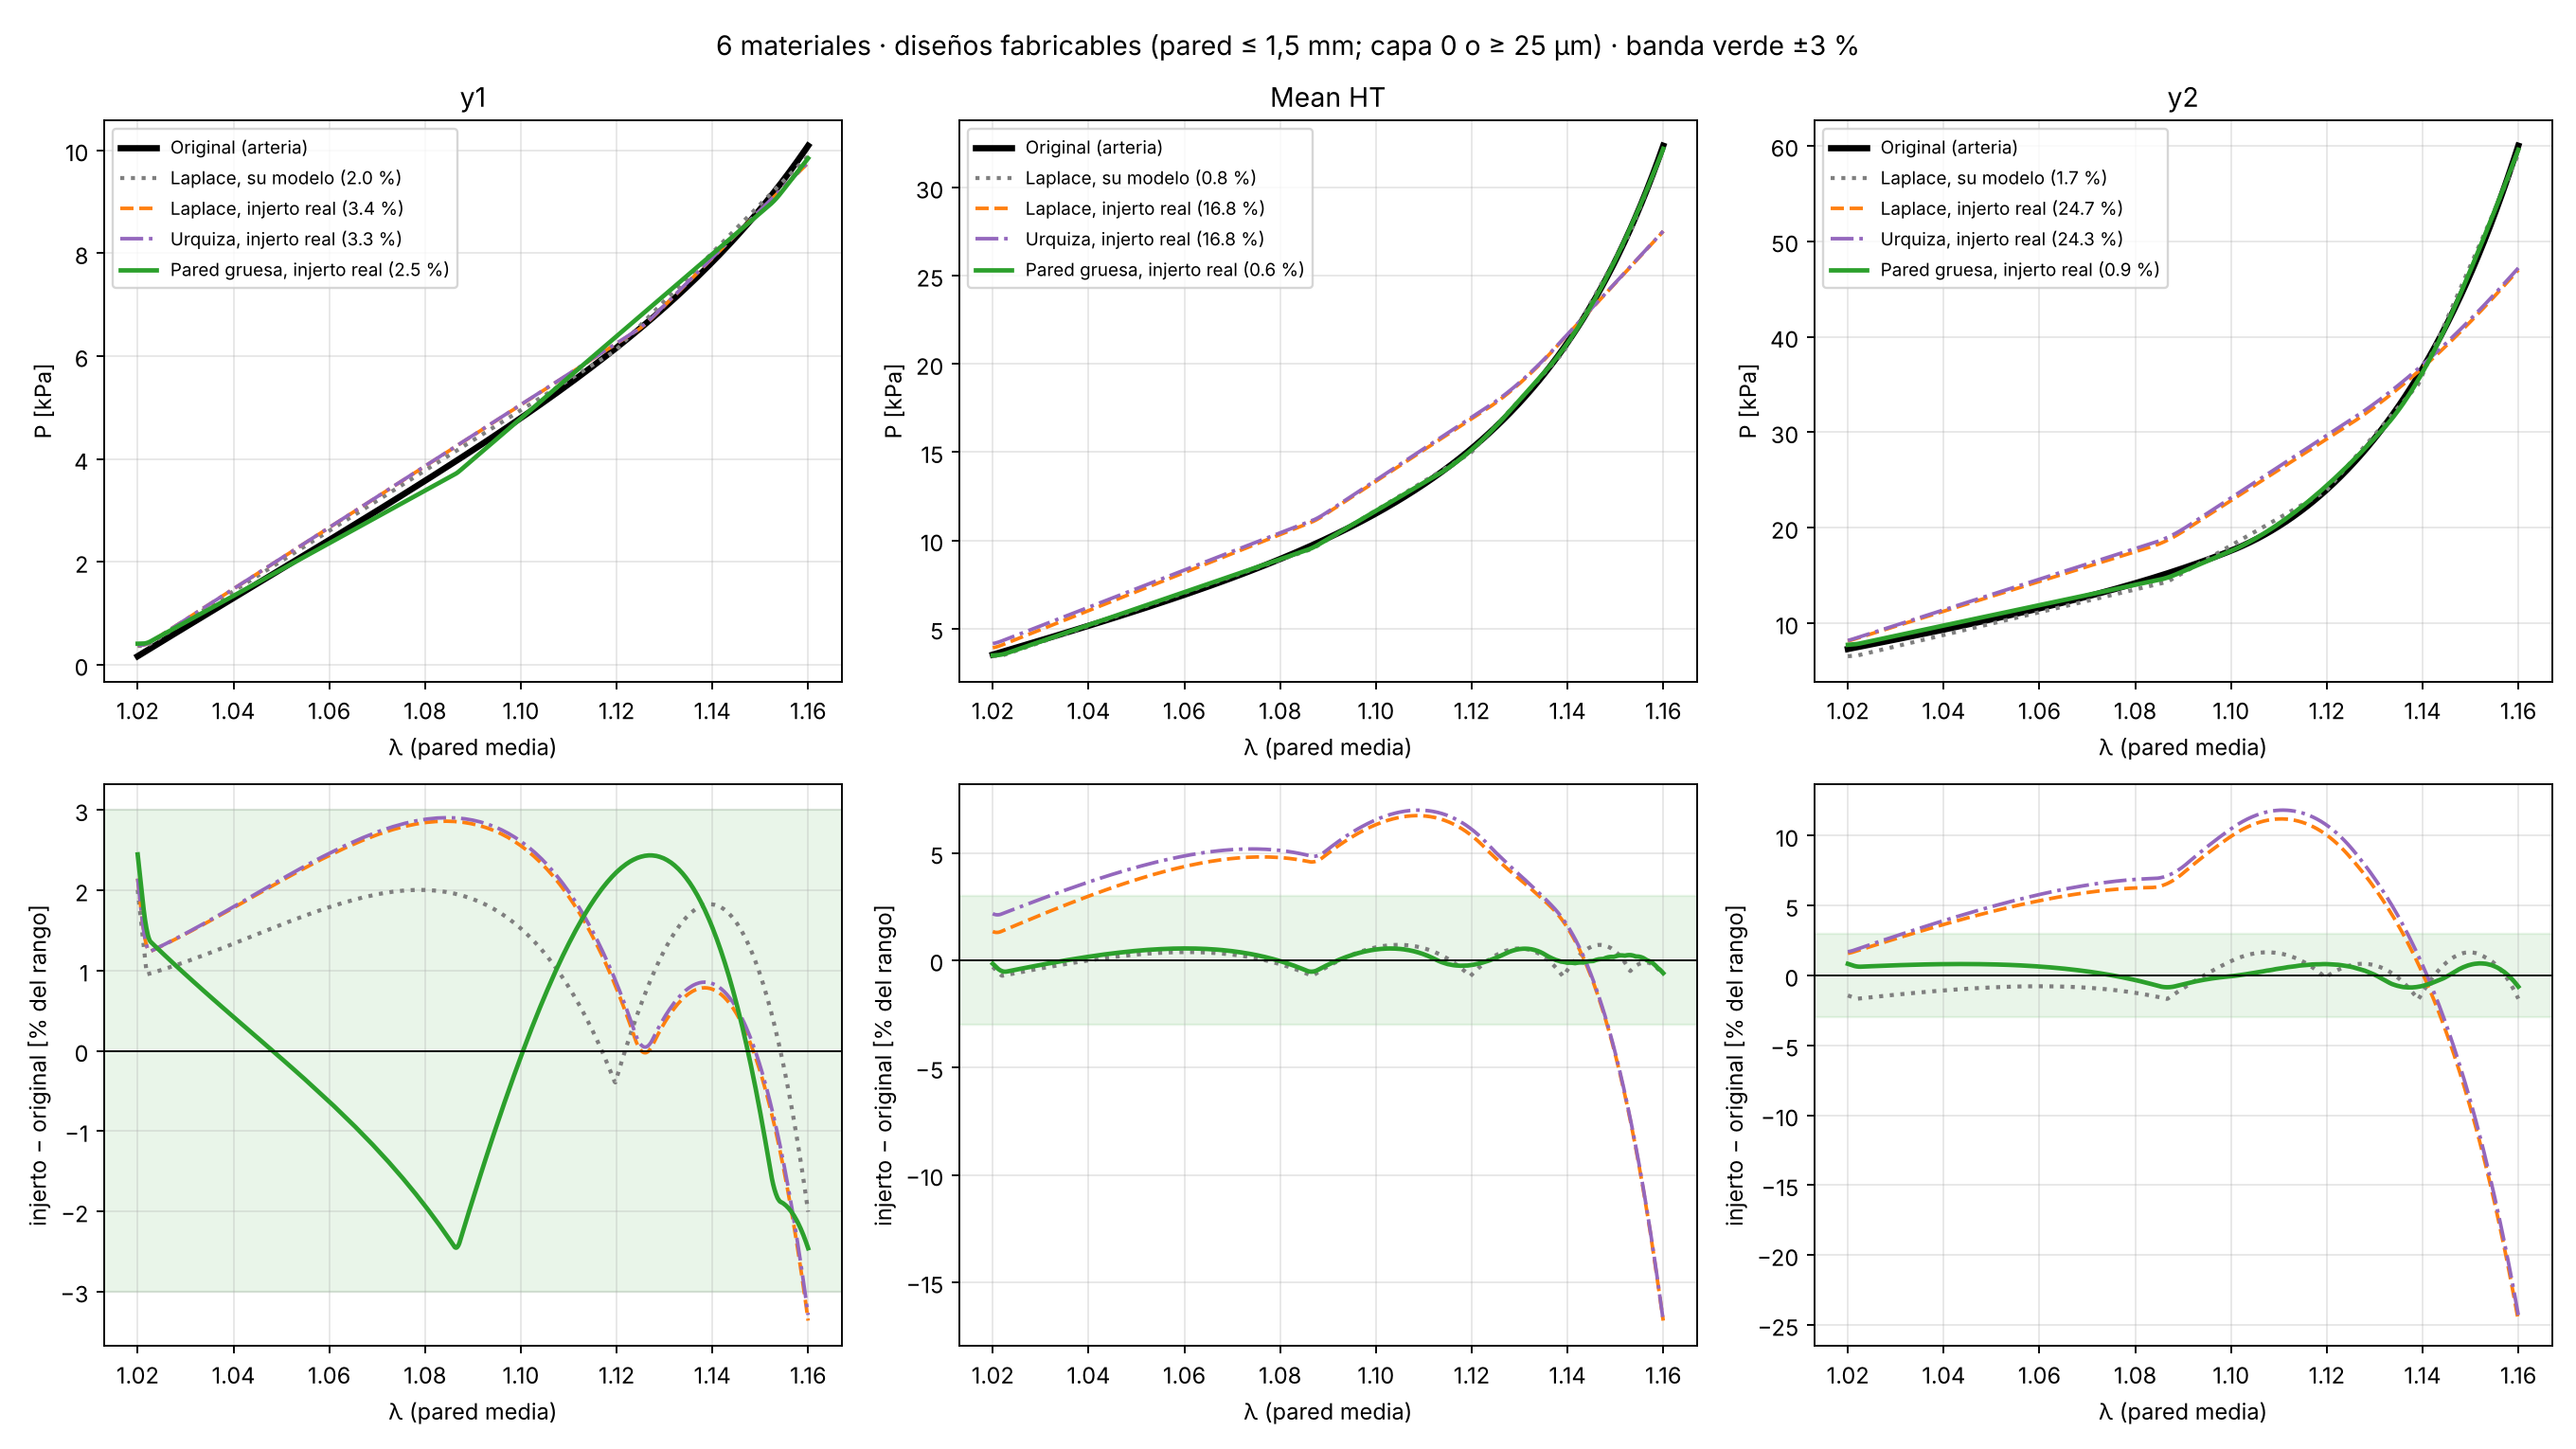
\includegraphics[width=0.82\textwidth]{f34_3c_6.png}
\caption{Tabla~\ref{tab:laplace}, 6 materiales, de izquierda a derecha: curva más blanda ($y_1$), media de los hipertensos y más rígida ($y_2$). Arriba de cada par: curvas; abajo: injerto $-$ arteria en \% del rango (banda $\pm3$\,\%). El diseño de Laplace evaluado en su propio modelo (gris, punteado) parece perfecto; fabricado (naranja, a trazos), se aparta hasta 25\,\%.}\label{fig:laplace}\end{figure}

\subsection{Qué se elige: las láminas de cada capa y el preestiramiento}
El injerto es un tubo con una capa por material, apiladas de adentro hacia afuera por nudo creciente. Los materiales son los del primer nivel: los mismos nudos y las mismas rectas, $\sigma_j=E_j\max(0,\lambda-\kappa_j)$. Para cada paciente se eligen dos cosas:
\begin{itemize}
\item \textbf{Las láminas de cada capa}, $n_1,\dots,n_N$: números enteros de 0 a 20, con láminas de 0,025\,mm. El espesor de la capa $j$ es $h_j=n_j\times0{,}025$\,mm.
\item \textbf{El preestiramiento} $\delta$: un número real que corre todos los nudos juntos. La capa $j$ empieza a tirar cuando la pared llega a $k_j+\delta$ en lugar de $k_j$. Con $\delta<0$ las capas se montan más tensas y tiran desde antes; con $\delta>0$, más flojas, y tiran desde después. Hace falta porque cada sujeto recorre su propio tramo de estiramiento (de 1,02 a 1,23): sin $\delta$ vería solo uno o dos nudos.
\end{itemize}
\textbf{Rigidez de los materiales.} El módulo $E_j$ de cada material se fija una sola vez para toda la población. Con láminas de 0,025\,mm, el tope de 20 láminas por material limita cada capa a 0,5\,mm; para que ningún sujeto lo supere, los materiales más rígidos se hicieron más rígidos: con 6 materiales, los materiales 4, 5 y 6 un 11, un 28 y un 50\,\% más; con 5, el material 5 un 50\,\% más. Con esos módulos, el sujeto que más láminas necesita usa 18 de un material (6 materiales) y 20 (5 materiales).

\subsection{Cómo se calcula el diseño: tres pasos}
Como la presión no es lineal en los espesores, el programa lineal del primer nivel ya no sirve. El diseño se calcula en tres pasos (Fig.~\ref{fig:proc}):
\begin{enumerate}
\item \textbf{Arranque de pared delgada}: un primer diseño con la ley de Laplace, que es lineal y se resuelve como en el primer nivel.
\item \textbf{Mínimos cuadrados en pared gruesa}: partiendo del arranque, se ajustan los espesores (números reales) y $\delta$ para que la curva del injerto se acerque a la del paciente. Como la curva de un injerto es suave, este paso también le quita el ruido a una curva medida.
\item \textbf{Láminas enteras por minimax}: cerca de los espesores del paso 2 se buscan las láminas enteras, y su $\delta$, que hacen más chico el peor error contra la curva del paso 2.
\end{enumerate}
Este procedimiento es la referencia a nivel del tubo, como el minimax lo es en el primer nivel; lo llamamos también \emph{minimax}. Los algoritmos de cada paso están en el Anexo~\ref{sec:calculo}.

\begin{figure}[H]\centering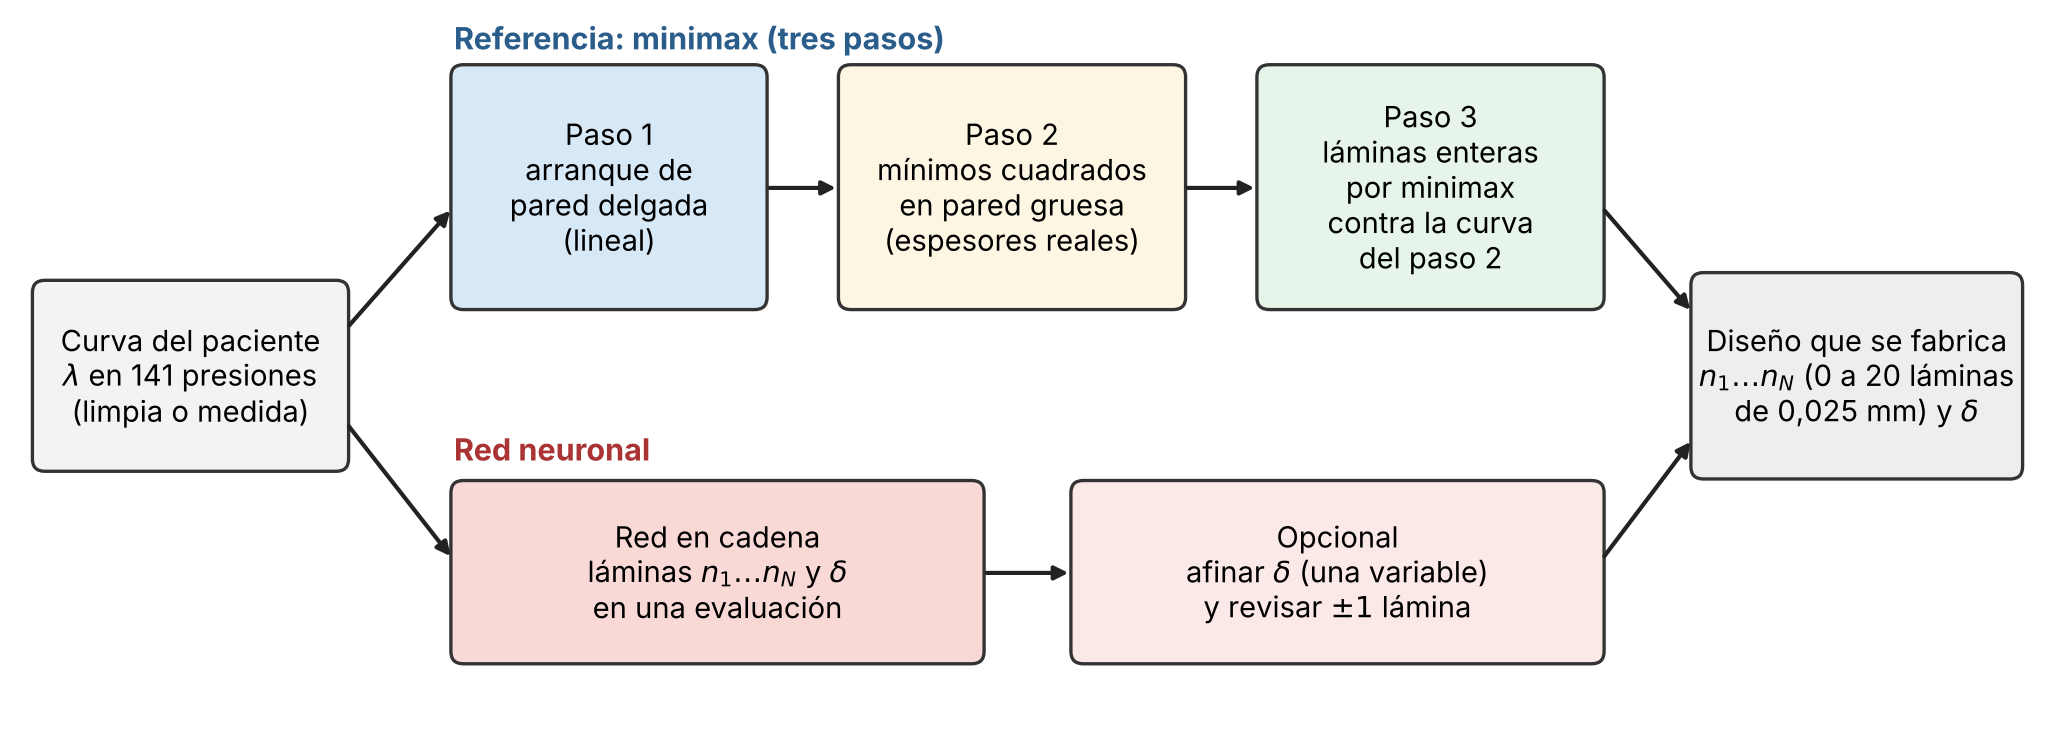
\includegraphics[width=\textwidth]{f_procedimiento_v59_es.png}
\caption{Dos maneras de obtener el diseño entero a nivel del tubo. Arriba, la referencia: tres pasos de optimización. Abajo, la red en cadena: una evaluación y, si se quiere, una revisión corta.}\label{fig:proc}\end{figure}

\subsection{La red en cadena para el tubo}
Se usa la misma red del primer nivel (Fig.~\ref{fig:cadena}), con dos cambios (Fig.~\ref{fig:cadenatubo}). (1) La entrada es la curva del paciente, el estiramiento $\lambda$ en los 141 valores de presión. (2) Tiene una cabeza más, que da $\delta$ después de que las otras eligieron las láminas. Cada cabeza $j$ responde las 20 preguntas ``¿más de $k$ láminas?'' y $n_j$ es la cantidad de respuestas afirmativas, igual que en el primer nivel.

\begin{figure}[H]\centering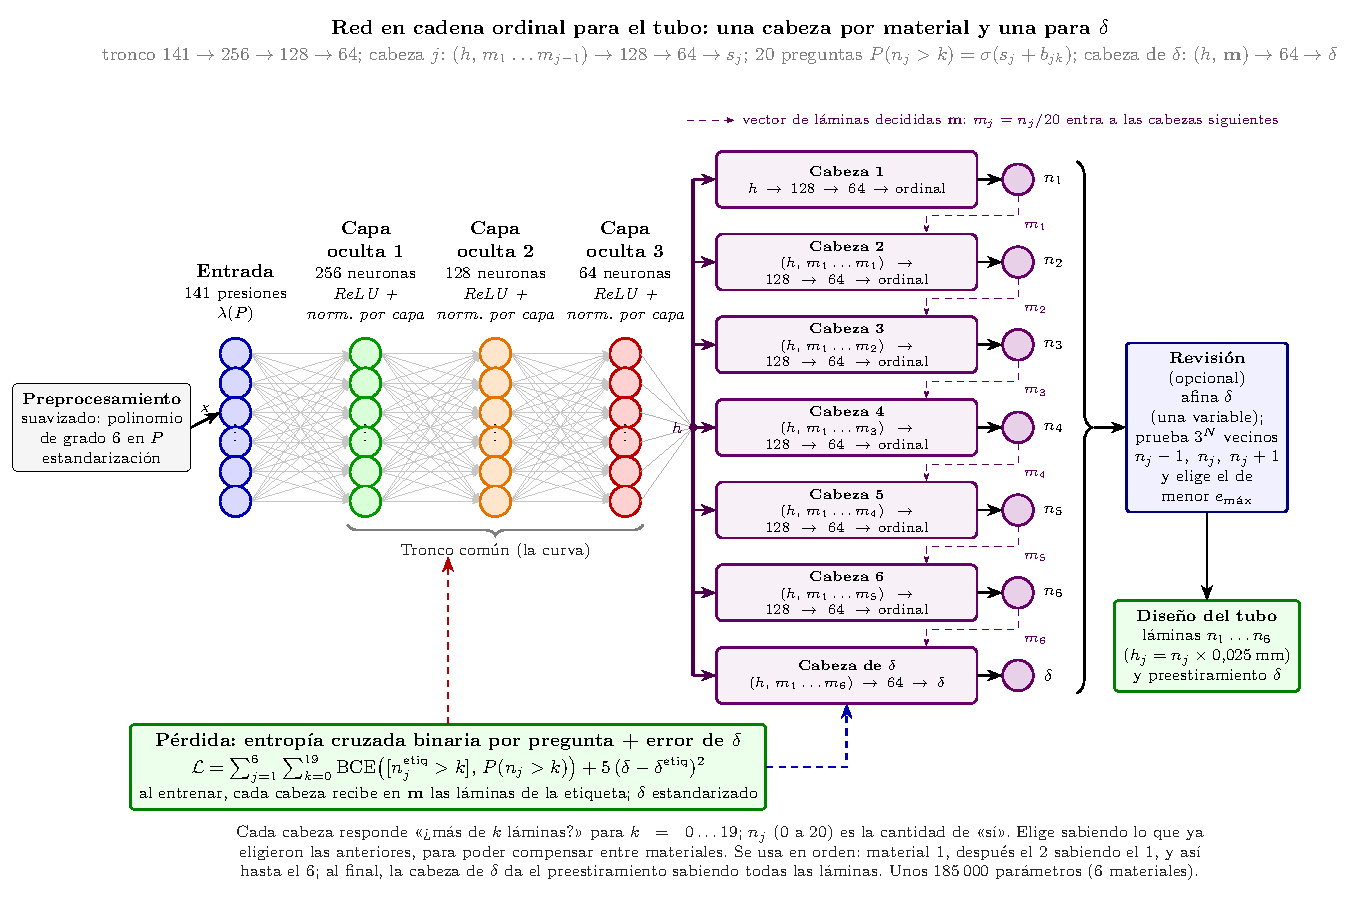
\includegraphics[width=\textwidth]{red_cadena_tubo_es.pdf}
\caption{Red en cadena del tubo (6 materiales). Es la red de la Fig.~\ref{fig:cadena} con otra entrada, la curva $\lambda(P)$ en 141 presiones, y una cabeza más: después de que las seis cabezas eligieron las láminas $n_1\ldots n_6$, la cabeza de $\delta$ recibe $h$ y el vector de láminas decididas $\mathbf{m}$ y da el preestiramiento.}\label{fig:cadenatubo}\end{figure}

\textbf{Con qué se entrena.} Con dos tipos de curvas: injertos con láminas y $\delta$ sorteados, cuya respuesta correcta es exactamente lo sorteado, y arterias sintéticas de la ley de Masson más los 31 sujetos de entrenamiento, cuya respuesta correcta es el diseño de los tres pasos. Los 10 sujetos de prueba no se usan.

\textbf{Cómo se usa.} La red da las láminas y $\delta$ en una evaluación. Después, con las láminas fijas, se puede afinar $\delta$, que es una sola variable. Y, como en el primer nivel, se puede revisar $\pm1$ lámina por material ($3^N$ combinaciones).

\subsection{Resultados}
La Tabla~\ref{tab:f2} resume los resultados con láminas enteras de 0,025\,mm, siempre contra la curva verdadera del sujeto. Como en el primer nivel, se presentan por separado los 31 sujetos de entrenamiento, los 10 de prueba, que la red nunca vio, y 300 arterias sintéticas de prueba.

\begin{table}[H]\centering\small
\caption{Nivel del tubo, láminas enteras de 0,025\,mm (a lo sumo 20 por material): curvas que cumplen la meta de 3\,\% y peor $e_{\max}$ [\%], contra la curva verdadera. Red $\pm1$: la red, $\delta$ afinado y la revisión de $\pm1$ lámina.}\label{tab:f2}
\resizebox{\textwidth}{!}{%
\begin{tabular}{lcccccc}\toprule
 & \multicolumn{3}{c}{6 materiales} & \multicolumn{3}{c}{5 materiales}\\\cmidrule(lr){2-4}\cmidrule(lr){5-7}
Curvas & minimax & red & red $\pm1$ & minimax & red & red $\pm1$\\\midrule
\multicolumn{7}{l}{\emph{Curvas limpias}}\\
Masson, entrenamiento (31) & 31/31 · 1,80 & 25/31 · 5,07 & 31/31 · 1,60 & 31/31 · 2,73 & 27/31 · 3,46 & 31/31 · 2,07\\
Masson, prueba (10) & 10/10 · 1,81 & 7/10 · 10,23 & 10/10 · 1,97 & 10/10 · 2,88 & 5/10 · 6,26 & 9/10 · 4,22\\
Arterias sintéticas de prueba (300) & 300/300 · 2,68 & 196/300 · 16,01 & 294/300 · 6,34 & 290/300 · 3,65 & 201/300 · 38,91 & 297/300 · 22,18\\\addlinespace
\multicolumn{7}{l}{\emph{Curvas medidas, 41 sujetos}}\\
10 presiones & 41/41 · 2,07 & 32/41 · 5,07 & 41/41 · 1,88 & 41/41 · 2,93 & 32/41 · 6,27 & 40/41 · 4,34\\
ruido 0,3\,\% & 24/41 · 14,14 & 19/41 · 21,00 & 29/41 · 6,10 & 21/41 · 17,81 & 14/41 · 15,44 & 28/41 · 6,07\\
10 presiones + ruido 0,2\,\% & 6/41 · 7,77 & 4/41 · 18,84 & 10/41 · 11,52 & 7/41 · 10,00 & 2/41 · 50,30 & 3/41 · 20,40\\\bottomrule
\end{tabular}}
\end{table}

\paragraph{Curvas limpias.} El minimax cumple la meta en los 41 sujetos, con 6 y con 5 materiales. La red sola no alcanza: con 6 materiales cumple en 32 de los 41. Con $\delta$ afinado y la revisión de $\pm1$ lámina cumple en los 41 con 6 materiales y en 40 con 5; el que falta, NT08 (4,22\,\%), es un sujeto de prueba en el que la red erró por una lámina en cuatro materiales a la vez, y la revisión de $\pm1$ no lo encontró. La Fig.~\ref{fig:emax59} muestra el peor error de cada sujeto y la Fig.~\ref{fig:dis59}, tres diseños. Las láminas de cada sujeto están en el Anexo~\ref{sec:tablas}.

\begin{figure}[H]\centering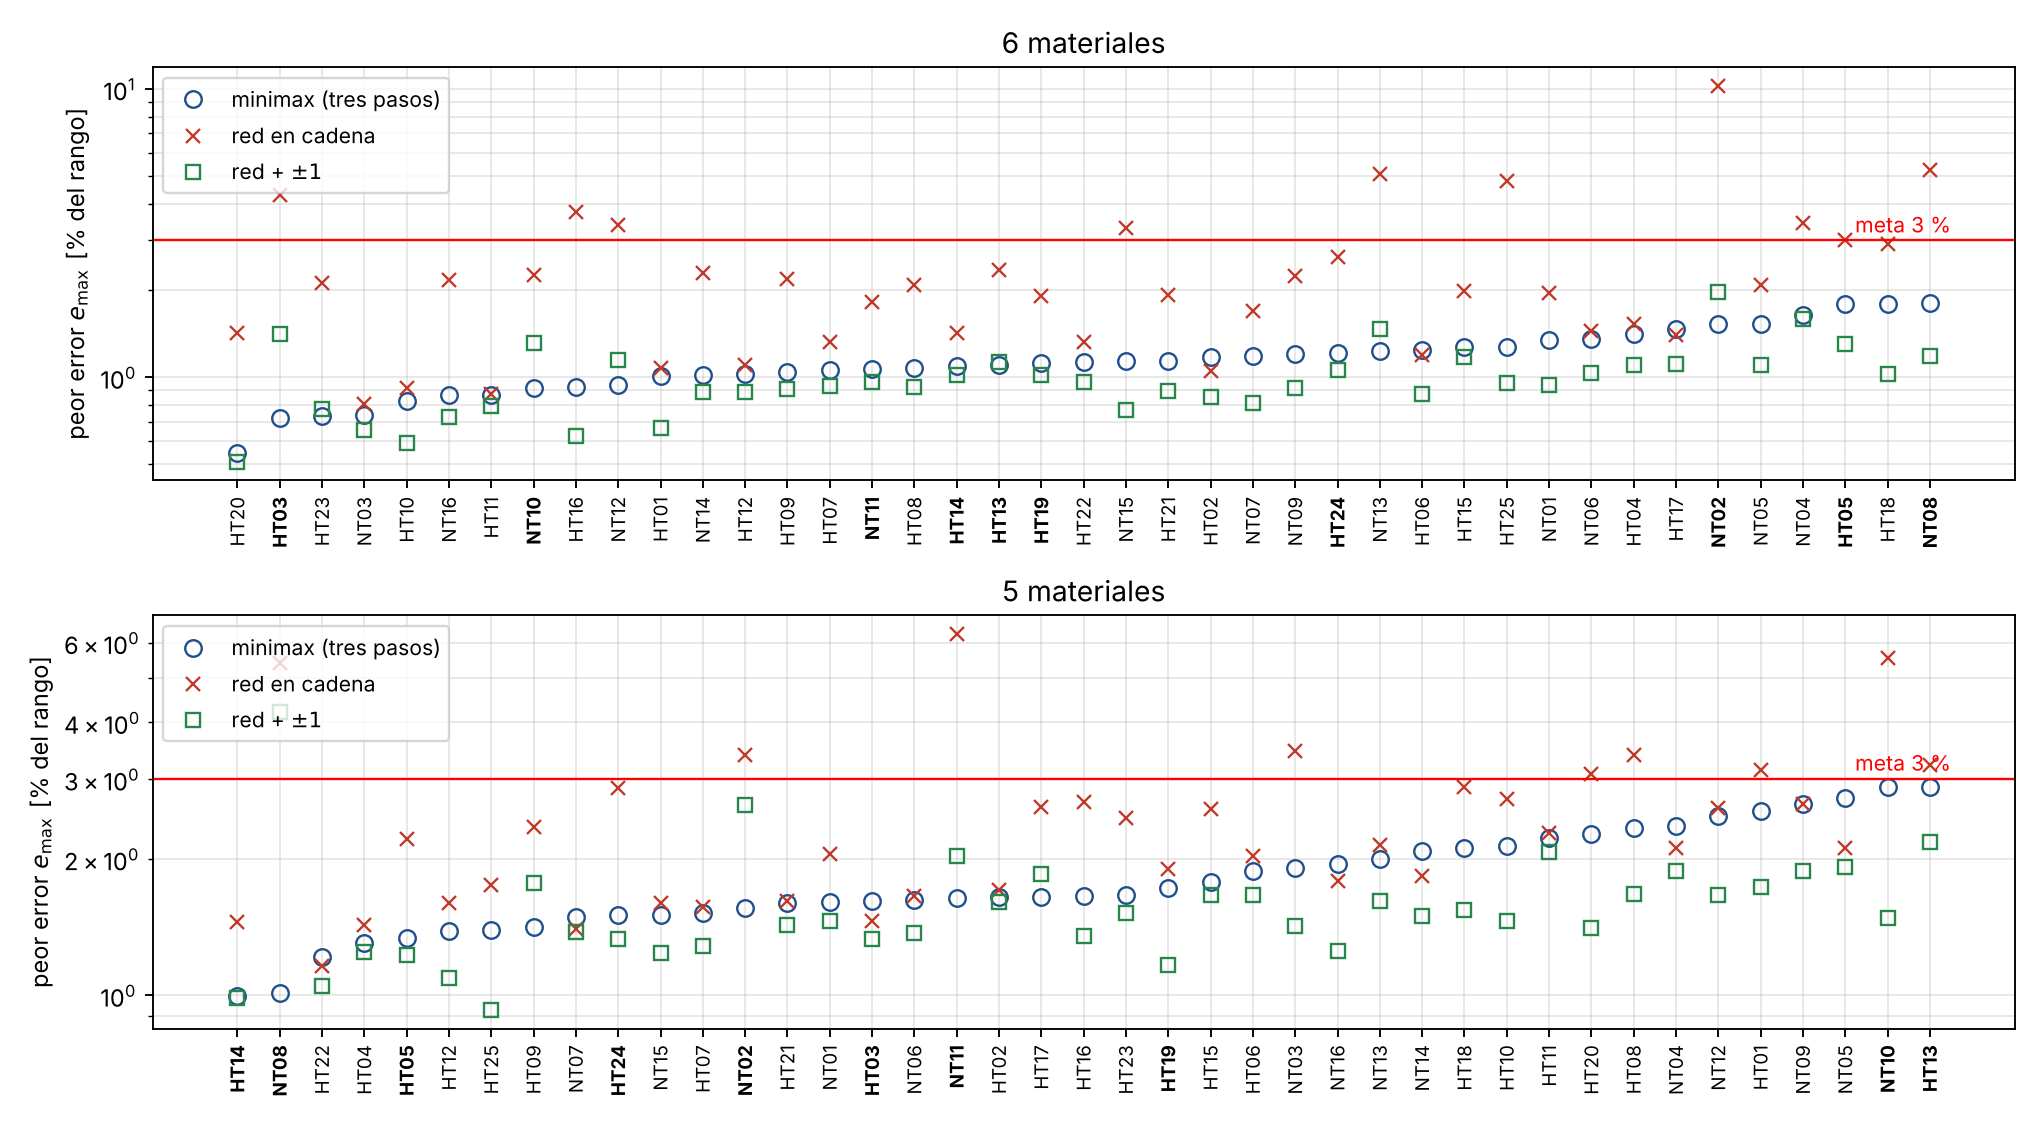
\includegraphics[width=\textwidth]{v59_emax_es.png}
\caption{Nivel del tubo: peor error de cada sujeto con láminas enteras, contra su curva $\lambda(P)$: minimax de tres pasos (círculos), red en cadena (cruces) y red con $\delta$ afinado y revisión de $\pm1$ (cuadrados). Sujetos ordenados por el error del minimax; en negrita, los de prueba. Línea roja: meta de 3\,\%.}\label{fig:emax59}\end{figure}

\begin{figure}[H]\centering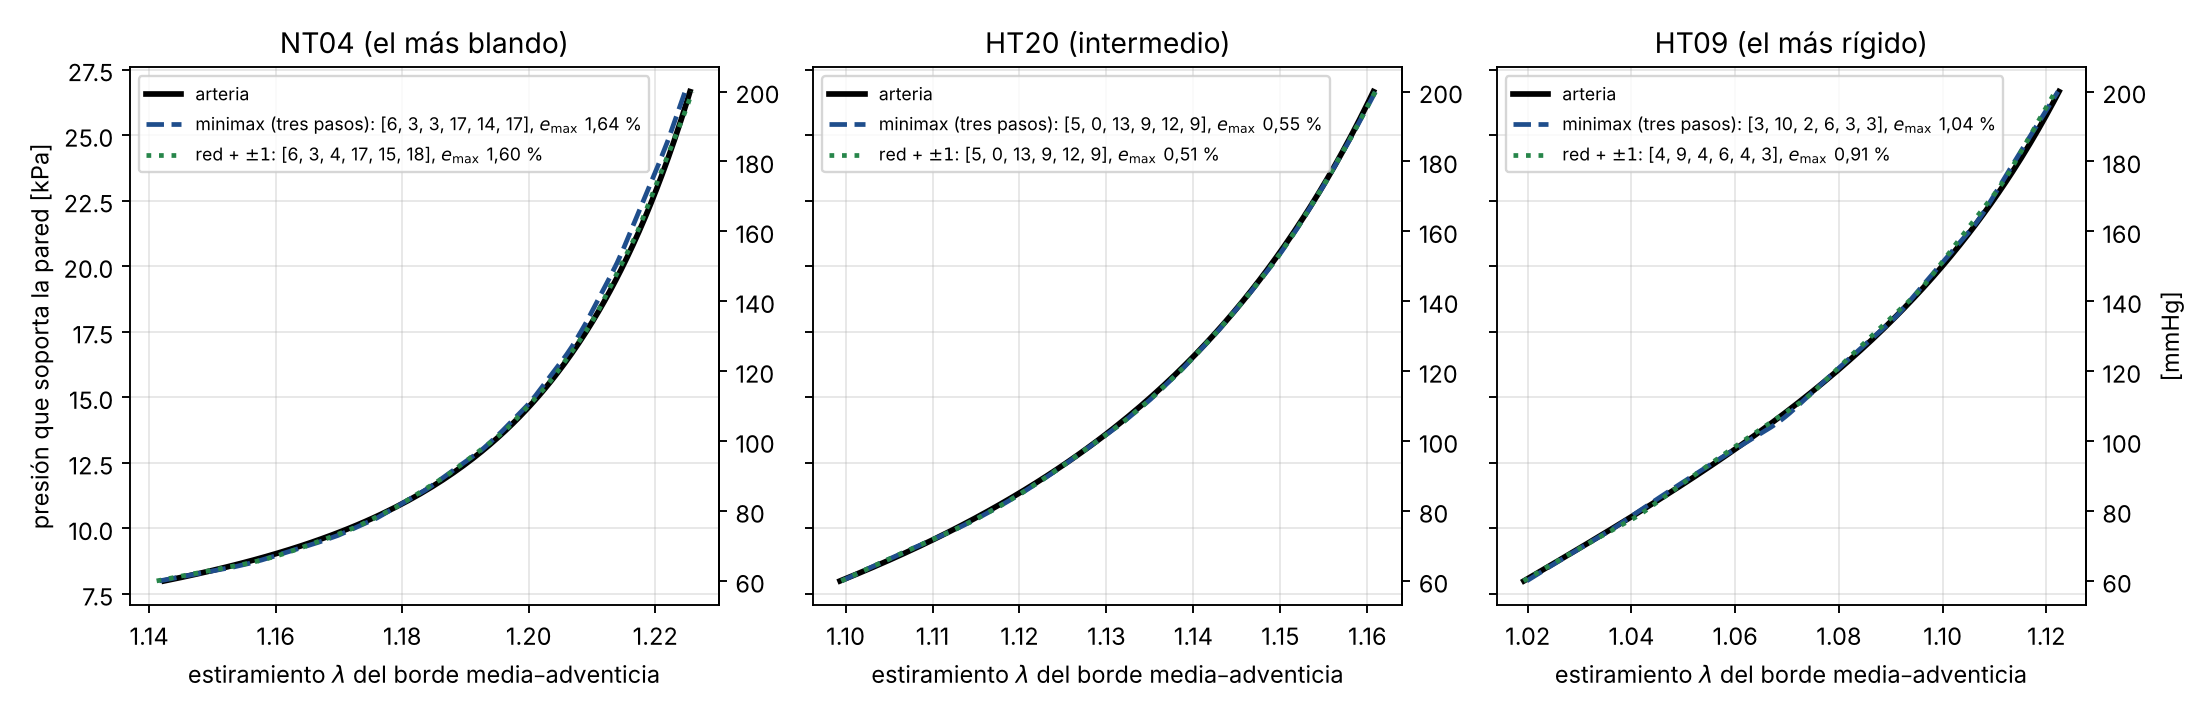
\includegraphics[width=\textwidth]{v59_disenos_es.png}
\caption{6 materiales, curvas limpias: el sujeto más blando, uno intermedio y el más rígido. Negra: arteria; azul, a trazos: minimax; verde, punteada: red $\pm1$. Ordenada: presión que soporta la pared, en kPa a la izquierda y en mmHg a la derecha. Entre corchetes, láminas de cada material, de la sangre hacia afuera.}\label{fig:dis59}\end{figure}

\paragraph{Muchos diseños sirven.} La red da exactamente las láminas del minimax solo en el 7\,\% de las arterias sintéticas de prueba con 6 materiales (26\,\% con 5), y aun así su diseño cumple la meta en 294 de 300. A nivel del tubo hay muchos diseños enteros con casi la misma curva: en HT09 (Fig.~\ref{fig:dis59}) el minimax y la red usan láminas distintas en cuatro materiales, y los dos cumplen con holgura (1,04 y 0,91\,\%). Por eso la red se juzga por el error en la curva y no por coincidir con el minimax.

\paragraph{Curvas medidas.} Antes de la red, la curva medida se suaviza con un polinomio de grado 6 en la presión, que no cambia una curva limpia (el minimax la suaviza en su paso 2). Con 10 presiones, los dos métodos cumplen en casi todos los sujetos. Con ruido de 0,3\,\%, que equivale a un 5\,\% del rango y es mayor que la meta, la red con revisión de $\pm1$ cumple en más sujetos que el minimax (29 contra 24 con 6 materiales; 28 contra 21 con 5) y su peor caso es menos de la mitad (6,1 contra 14,1\,\% con 6 materiales y 6,1 contra 17,8\,\% con 5). Con 10 presiones y ruido ningún método pasa de 10 de 41: ahí el límite es la medición.

\paragraph{Tiempo.} Los dos métodos tardan menos de un segundo por sujeto: con 6 materiales, 0,55\,s el minimax y 0,60\,s la red con la revisión de $\pm1$.

%=====================================================================
\section{Discusión}
\paragraph{Por qué dos niveles.} La curva tensión--estiramiento es una propiedad del tejido. Trabajar primero sobre ella permite validar cada pieza del método ---la base, el ajuste, el redondeo, la red--- contra soluciones exactas, sin que intervengan la geometría ni la presión, que dependen de cada arteria y de cada sitio. El paso al tubo agrega la geometría y la hipótesis de pared gruesa, pero conserva los materiales, la métrica, el criterio minimax y la conclusión sobre el ruido.

\paragraph{Generalidad.} Lo que se valida en el primer nivel no es propio de la carótida: los materiales tipo fibra, la base elegida sobre un espacio amplio de curvas en J, el diseño entero minimax y una red que da ese diseño en curvas de leyes que nunca vio. Para otra arteria cambian la geometría, el espesor y la ventana de presión, que entran recién en el segundo nivel; la franja de curvas y, si hiciera falta, los nudos se recalculan con el mismo procedimiento, y la red se reentrena dentro de la nueva franja. La validación externa (Sección~\ref{sec:externa}) lo confirma con datos: la base elegida con las carótidas de Masson reproduce, sin cambios, curvas de carótida común, externa e interna, de paredes intactas y media--íntimas y de pacientes con placa, de tres leyes constitutivas distintas, cada una en su ventana de presión. Lo que limita en algunas curvas in vivo es la división en 20 láminas por material frente a un recorrido de tensión pequeño, no la forma de la curva ni la red.

\paragraph{El papel de la red neuronal.} En el primer nivel, el minimax da el mejor diseño entero, pero resolviendo un problema de optimización por cada curva. La red en cadena da el diseño entero directamente, con la misma operación para cualquier curva de su dominio de validez: sola, cumple la meta en los 41 sujetos (6 materiales); con una búsqueda de $\pm1$ lámina, que solo evalúa 729 combinaciones, llega a 91 de los 98 casos que admiten un diseño entero dentro de la meta. No tiene la garantía de óptimo del minimax, que sigue siendo la referencia para comprobar cualquier diseño, y no se usa fuera de la franja $y_1$--$y_2$, donde no puede asegurar la meta. En el tubo de pared gruesa la misma red, con la misma salida ordinal, da las láminas de cada capa y el preestiramiento; con la revisión de $\pm1$ lámina iguala al procedimiento de tres pasos con curvas limpias y lo supera con curvas con ruido, porque elige entre diseños vistos en el entrenamiento y no persigue el ruido. Es la idea de la optimización amortizada~\cite{amos}: un modelo aprendido sobre muchos casos resueltos da la solución de uno nuevo, y una búsqueda corta la termina. La red no reemplaza al minimax como referencia para comprobar un diseño.

\paragraph{Por qué pared gruesa.} La diferencia entre los modelos está en una sola hipótesis: en pared delgada todas las fibras se estiran igual; en pared gruesa cada una tiene su estiramiento, fijado por la incompresibilidad. Con materiales que no tiran hasta su nudo, esa diferencia de pocos centésimos decide si una capa trabaja. El enganche de cada capa (su rizado) es tan importante como su espesor: entre un diseño de Laplace y uno de pared gruesa los espesores cambian pocos micrómetros, pero las capas externas enganchan antes.

\paragraph{Limitaciones.} (1) Las curvas objetivo son las de la ley ajustada por Masson et al., no las mediciones crudas, y el espesor arterial es el de referencia para la edad y el sexo. (2) Los materiales son ideales (rectas truncadas de rigidez constante); el injerto no tiene alargamiento axial ni tensiones residuales, y no se consideran viscoelasticidad ni fatiga. (3) La búsqueda entera en pared gruesa es heurística: queda a menos de medio punto del óptimo en una vecindad de $\pm2$ láminas, pero no se demostró el óptimo global; se usó una sola realización de ruido por sujeto y caso. Para respetar el tope de 20 láminas se aumentó la rigidez de los materiales más rígidos, lo que deberá verificarse con materiales reales. (4) El preestiramiento $\delta$ y el rizado por capa son variables de fabricación que deben validarse. (5) La red del primer nivel vale dentro de la franja $y_1$--$y_2$ de la población de Masson; para curvas fuera de ella hay que ampliar la franja y reentrenarla, o usar solo el minimax. (6) No hay validación experimental.

%=====================================================================
\section{Conclusiones}
\begin{enumerate}
\item Un injerto de capas de materiales tipo fibra (rectas truncadas), con una base elegida una vez para toda la población y a lo sumo 20 láminas por material, reproduce la curva tensión--estiramiento de 41 carótidas humanas: con 6 materiales y láminas enteras por minimax, los 41 sujetos cumplen la meta de 3\,\%.
\item Una sola red neuronal, en cadena y con salida ordinal, entrenada dentro de la franja $y_1$--$y_2$ ---su dominio de validez---, da directamente las láminas enteras en una evaluación, sin optimizar. Con una búsqueda de $\pm1$ lámina cumple la meta en los 31 sujetos de entrenamiento y en los 10 de prueba, con 6 y con 5 materiales salvo un sujeto que tampoco cumple con el minimax.
\item Sin ningún cambio, la misma base y la misma red se aplicaron a 63 curvas de otros tres estudios (Sommer y Holzapfel, Liu et al., Kamenskiy et al.) dentro del dominio de validez, cada una con su ley constitutiva y su ventana de presión: con 6 materiales, la red con búsqueda de $\pm1$ cumple en 50 y el minimax en 57; en las otras 6 ningún diseño entero cumple, porque su recorrido de tensión es pequeño frente al paso de una lámina. Sumando los 104 casos, la red llega a 91 de los 98 alcanzables con láminas enteras.
\item A nivel del tubo el diseño debe hacerse en pared gruesa: diseñado con la ley de Laplace, ningún sujeto cumple al fabricarse; en pared gruesa cumplen los 41. El problema es no lineal entero.
\item Con láminas de 0,025\,mm y a lo sumo 20 por material, el procedimiento de tres pasos ---arranque, mínimos cuadrados no lineales y minimax entero--- cumple en los 41 sujetos, con 6 y con 5 materiales, en menos de un segundo por sujeto.
\item La misma red en cadena, entrenada para el tubo, da las láminas de cada capa en una evaluación; con $\delta$ afinado y una revisión de $\pm1$ lámina cumple en los 41 sujetos con 6 materiales y en 40 con 5. Con curvas medidas con ruido cumple en más sujetos que el minimax (29 contra 24 con 6 materiales) y con un peor caso menor. Una sola red sirve así para los dos niveles.
\end{enumerate}
\paragraph{Próximos pasos.} Probar el método con curvas medidas de otras arterias; ensayar materiales reales para reemplazar las rectas ideales y validar el rizado como variable de fabricación; usar el espesor y la presión medidos de cada sujeto; y fabricar y ensayar un injerto.

%=====================================================================
\appendix
\section{Parámetros de los 41 sujetos}\label{sec:anexo}
\begin{table}[H]\centering\scriptsize
\caption{Parámetros de Masson et al.~\cite{masson} (sus Tablas 2 y 4). $^\dagger$: sujeto reservado para prueba.}\label{tab:masson}
\resizebox{\textwidth}{!}{%
\begin{tabular}{lcccccccccccccccc}\toprule
Sujeto & Edad & Sexo & $R_m$ & $\Theta_0$ & $\lambda_z$ & $c$ & $c_1$ & $c_2$ & $c_1^{\mathrm{circ}}$ & $c_2^{\mathrm{circ}}$ & $\alpha$ & $T_m$ & $\lambda_0$ & $\lambda_m$ & $a$ & $b$\\
 & [años] & & [mm] & [°] & & [kPa] & [kPa] & & [kPa] & & [°] & [kPa] & & & [kPa] & \\\midrule
NT01 & 62 & F & 4,26 & 128,70 & 1,11 & 29,82 & 9,44 & 14,14 & 16,13 & 15,11 & 65,74 & 39,73 & 0,960 & 1,70 & 0,122 & 3,52\\
NT02$^\dagger$ & 60 & M & 4,69 & 128,90 & 1,08 & 20,42 & 8,47 & 13,10 & 14,16 & 15,12 & 44,46 & 41,84 & 0,680 & 1,92 & 0,126 & 3,40\\
NT03 & 31 & M & 4,30 & 132,20 & 1,09 & 27,23 & 10,34 & 13,10 & 7,01 & 12,82 & 48,62 & 43,37 & 0,820 & 1,65 & 0,139 & 3,57\\
NT04 & 31 & M & 4,67 & 133,90 & 1,10 & 23,59 & 6,58 & 11,77 & 6,38 & 10,69 & 32,04 & 39,81 & 0,680 & 1,59 & 0,118 & 3,53\\
NT05 & 34 & F & 4,20 & 130,10 & 1,10 & 35,68 & 13,62 & 13,18 & 13,38 & 13,17 & 50,72 & 50,07 & 0,860 & 1,62 & 0,103 & 3,58\\
NT06 & 53 & F & 3,96 & 130,10 & 1,11 & 33,37 & 11,38 & 13,63 & 13,30 & 14,26 & 57,14 & 46,59 & 0,950 & 1,69 & 0,093 & 3,44\\
NT07 & 21 & F & 3,83 & 132,00 & 1,10 & 44,28 & 21,79 & 13,17 & 8,27 & 12,73 & 51,15 & 53,58 & 0,920 & 1,62 & 0,111 & 3,58\\
NT08$^\dagger$ & 25 & M & 4,86 & 133,20 & 1,07 & 23,25 & 6,34 & 12,93 & 8,11 & 13,17 & 42,93 & 31,90 & 0,820 & 1,77 & 0,173 & 3,57\\
NT09 & 42 & F & 4,51 & 129,50 & 1,10 & 34,90 & 16,14 & 13,58 & 19,64 & 13,89 & 57,21 & 47,01 & 0,930 & 1,65 & 0,084 & 3,55\\
NT10$^\dagger$ & 55 & M & 4,77 & 129,10 & 1,10 & 38,57 & 36,31 & 13,31 & 56,88 & 13,61 & 54,22 & 46,36 & 0,890 & 1,66 & 0,006 & 3,75\\
NT11$^\dagger$ & 64 & M & 5,57 & 129,50 & 1,10 & 34,89 & 40,16 & 13,45 & 66,88 & 13,53 & 54,54 & 41,12 & 0,850 & 1,79 & 0,005 & 3,23\\
NT12 & 60 & F & 4,88 & 130,10 & 1,09 & 33,94 & 10,78 & 13,95 & 12,79 & 15,42 & 60,97 & 45,77 & 0,930 & 1,73 & 0,099 & 3,37\\
NT13 & 61 & F & 4,92 & 130,60 & 1,09 & 35,15 & 17,69 & 13,43 & 18,40 & 13,22 & 55,04 & 45,59 & 0,940 & 1,66 & 0,085 & 3,51\\
NT14 & 39 & F & 3,54 & 131,50 & 1,09 & 28,97 & 8,22 & 13,13 & 19,02 & 13,16 & 50,22 & 41,30 & 0,890 & 1,67 & 0,105 & 3,53\\
NT15 & 58 & F & 3,92 & 132,40 & 1,08 & 26,71 & 15,79 & 13,36 & 16,68 & 13,11 & 53,60 & 35,32 & 0,950 & 1,71 & 0,166 & 3,60\\
NT16 & 60 & M & 5,72 & 129,70 & 1,10 & 27,79 & 28,23 & 13,46 & 57,77 & 13,63 & 55,73 & 36,50 & 1,05 & 1,77 & 0,141 & 3,58\\
HT01 & 68 & M & 4,96 & 130,90 & 1,10 & 35,91 & 12,57 & 14,08 & 15,52 & 14,91 & 67,18 & 48,42 & 0,990 & 1,66 & 0,098 & 3,50\\
HT02 & 54 & M & 4,93 & 129,80 & 1,10 & 38,20 & 16,40 & 13,20 & 16,44 & 13,20 & 51,11 & 52,44 & 0,860 & 1,62 & 0,137 & 3,58\\
HT03$^\dagger$ & 64 & F & 4,87 & 129,50 & 1,10 & 36,01 & 14,55 & 13,96 & 18,35 & 14,48 & 62,66 & 47,02 & 1,00 & 1,74 & 0,113 & 3,62\\
HT04 & 58 & F & 4,57 & 131,20 & 1,09 & 22,42 & 8,57 & 13,03 & 6,43 & 13,36 & 46,38 & 38,53 & 0,810 & 1,68 & 0,099 & 3,51\\
HT05$^\dagger$ & 62 & F & 4,78 & 130,10 & 1,10 & 48,19 & 35,06 & 13,23 & 43,19 & 13,03 & 53,24 & 52,86 & 0,910 & 1,63 & 0,033 & 3,56\\
HT06 & 66 & F & 5,06 & 129,10 & 1,10 & 39,78 & 37,75 & 13,35 & 60,89 & 13,45 & 56,01 & 46,44 & 0,910 & 1,64 & 0,004 & 3,54\\
HT07 & 54 & F & 4,30 & 129,60 & 1,11 & 50,45 & 25,51 & 13,32 & 39,43 & 13,24 & 53,47 & 64,91 & 0,930 & 1,66 & 0,078 & 3,72\\
HT08 & 63 & F & 4,44 & 129,00 & 1,10 & 34,44 & 30,62 & 13,29 & 60,33 & 13,21 & 54,67 & 44,94 & 0,930 & 1,65 & 0,084 & 3,56\\
HT09 & 68 & M & 5,09 & 128,20 & 1,12 & 51,48 & 33,77 & 13,17 & 44,26 & 13,49 & 51,83 & 66,41 & 0,840 & 1,62 & 0,023 & 3,55\\
HT10 & 55 & F & 4,30 & 129,00 & 1,10 & 37,04 & 12,32 & 14,13 & 15,04 & 14,93 & 65,14 & 48,19 & 1,04 & 1,71 & 0,114 & 3,47\\
HT11 & 69 & M & 5,54 & 131,20 & 1,08 & 29,64 & 9,76 & 13,23 & 9,10 & 15,12 & 48,16 & 37,83 & 0,830 & 1,74 & 0,115 & 3,59\\
HT12 & 54 & M & 5,43 & 131,80 & 1,09 & 32,23 & 17,81 & 13,35 & 14,03 & 12,15 & 53,73 & 44,93 & 0,920 & 1,65 & 0,090 & 3,58\\
HT13$^\dagger$ & 61 & M & 5,17 & 128,40 & 1,11 & 30,45 & 15,87 & 13,08 & 23,03 & 13,84 & 47,86 & 52,58 & 0,750 & 1,61 & 0,009 & 3,49\\
HT14$^\dagger$ & 60 & M & 4,64 & 129,90 & 1,10 & 30,43 & 13,74 & 13,45 & 18,01 & 13,35 & 54,90 & 42,43 & 0,910 & 1,66 & 0,088 & 3,52\\
HT15 & 53 & M & 4,65 & 130,40 & 1,10 & 40,83 & 28,98 & 13,36 & 31,16 & 12,62 & 54,44 & 49,57 & 0,930 & 1,65 & 0,085 & 3,63\\
HT16 & 54 & M & 4,71 & 129,60 & 1,10 & 45,26 & 29,27 & 14,00 & 33,48 & 14,82 & 67,16 & 67,68 & 1,02 & 1,65 & 0,039 & 3,52\\
HT17 & 53 & M & 5,04 & 130,00 & 1,10 & 37,25 & 39,18 & 13,24 & 66,29 & 13,15 & 54,90 & 48,26 & 0,910 & 1,64 & 0,099 & 3,60\\
HT18 & 52 & M & 4,92 & 129,70 & 1,10 & 29,28 & 10,50 & 13,21 & 19,76 & 13,39 & 50,96 & 46,42 & 0,850 & 1,63 & 0,094 & 3,56\\
HT19$^\dagger$ & 57 & F & 4,27 & 130,30 & 1,10 & 33,49 & 14,47 & 13,22 & 17,35 & 13,27 & 53,18 & 46,18 & 0,900 & 1,64 & 0,097 & 3,55\\
HT20 & 61 & F & 5,14 & 129,20 & 1,10 & 40,09 & 15,72 & 14,09 & 16,78 & 14,83 & 65,17 & 53,40 & 1,04 & 1,70 & 0,100 & 3,47\\
HT21 & 57 & F & 4,88 & 129,90 & 1,10 & 35,31 & 14,57 & 13,26 & 15,58 & 13,30 & 52,07 & 48,97 & 0,870 & 1,63 & 0,094 & 3,57\\
HT22 & 44 & F & 4,17 & 131,00 & 1,10 & 55,25 & 35,78 & 13,23 & 19,51 & 12,55 & 52,36 & 59,58 & 0,930 & 1,61 & 0,097 & 3,61\\
HT23 & 51 & M & 4,83 & 130,60 & 1,08 & 30,77 & 12,80 & 13,60 & 41,10 & 14,20 & 49,79 & 41,06 & 0,870 & 1,90 & 0,094 & 3,56\\
HT24$^\dagger$ & 65 & M & 4,57 & 129,60 & 1,10 & 38,91 & 25,76 & 13,20 & 35,01 & 13,20 & 51,94 & 50,28 & 0,870 & 1,62 & 0,043 & 3,58\\
HT25 & 67 & F & 4,72 & 129,20 & 1,10 & 40,29 & 31,78 & 13,75 & 60,40 & 14,29 & 63,50 & 46,06 & 1,03 & 1,72 & 0,025 & 3,46\\
\bottomrule\end{tabular}}
\end{table}


\section{Ejemplo de diseño de pared gruesa, paso a paso}\label{sec:ejemplo}
Este anexo muestra, con números que se pueden verificar con calculadora, las ideas que usa la Sección~\ref{sec:aplicacion}: el injerto reproduce el comportamiento de la arteria con capas de distintos materiales; cada fibra de una pared gruesa se estira distinto; la presión es la suma de los aportes de rebanadas delgadas; el lugar de cada capa cambia lo que aporta; y el preestiramiento $\delta$ corre todos los nudos. Para que las cuentas sean cortas el tubo es cerrado, sin tensiones residuales y sin alargamiento axial, y el nudo de cada material se aplica directamente al estiramiento local de cada franja (en el modelo completo el nudo se define en la pared media y se traduce a cada capa por incompresibilidad, ec.~\ref{eq:incomp}).

\subsection{La arteria y el injerto}
\begin{figure}[H]\centering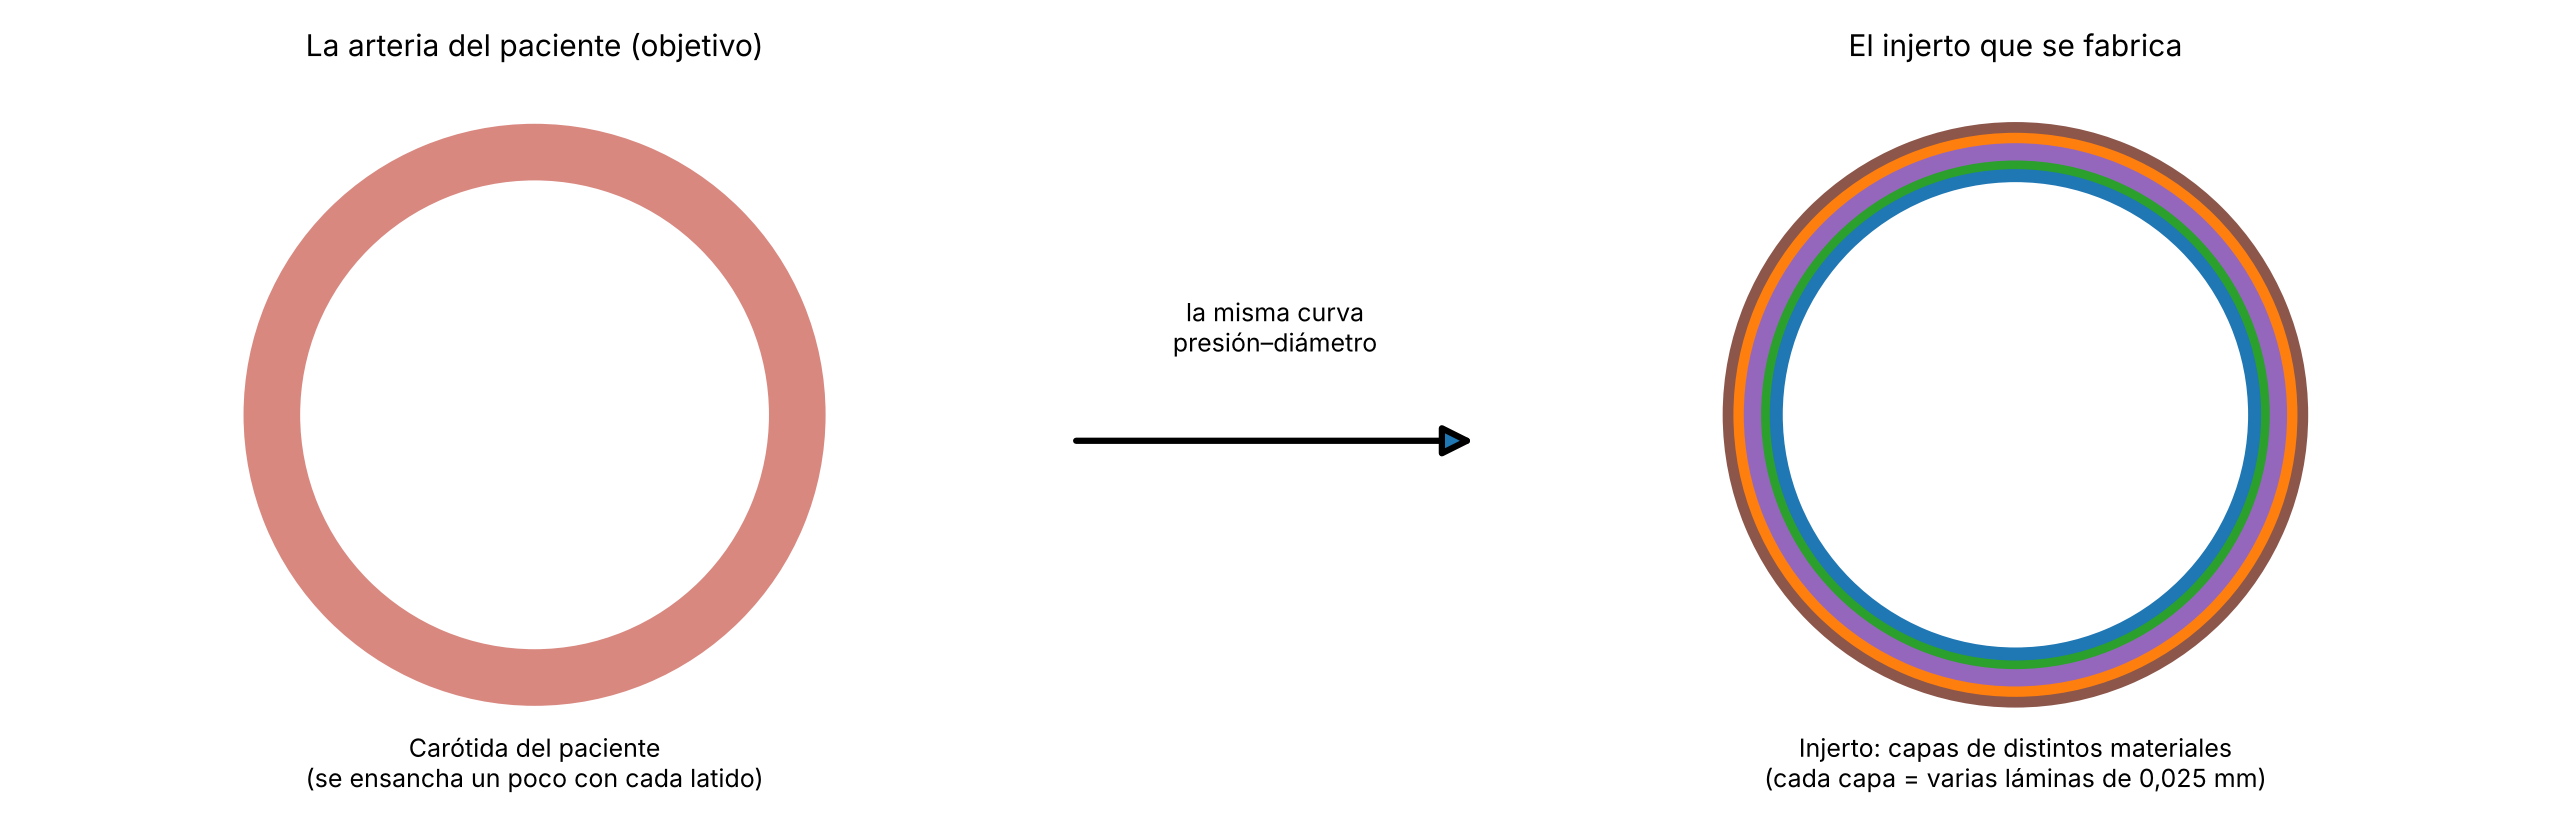
\includegraphics[width=0.85\textwidth]{d12_objetivo_v2.png}
\caption{La carótida del paciente (izquierda) y el injerto (derecha), hecho de capas de distintos materiales, cada capa con un número entero de láminas. El objetivo es que el injerto tenga la misma curva presión--diámetro que la arteria: que los dos se ensanchen igual con la presión.}\end{figure}

\subsection{Incompresibilidad: el área del anillo no cambia}
El tejido es casi todo agua: se deforma sin cambiar de volumen. Si el tubo no se alarga, el área del anillo es la misma antes y después de inflarlo:
\[
\pi\,(R_o^2-R_i^2)=\pi\,(r_o^2-r_i^2)\qquad\Longrightarrow\qquad r=\sqrt{r_i^2+R^2-R_i^2}\quad\text{para cualquier radio }R\text{ de la pared.}
\]
Tubo de ejemplo: sin presión de $R_i=3{,}0$ a $R_o=3{,}6$\,mm; con presión la cara interna llega a $r_i=3{,}3$\,mm. Entonces $r=\sqrt{1{,}89+R^2}$ (porque $3{,}3^2-3{,}0^2=1{,}89$) y $r_o=\sqrt{14{,}85}=3{,}854$\,mm. La cara interna se estira $3{,}3/3{,}0=1{,}100$ y la externa $3{,}854/3{,}6=1{,}070$ (Fig.~\ref{fig:fibra}): \textbf{en pared gruesa no hay un solo estiramiento}.
\begin{figure}[H]\centering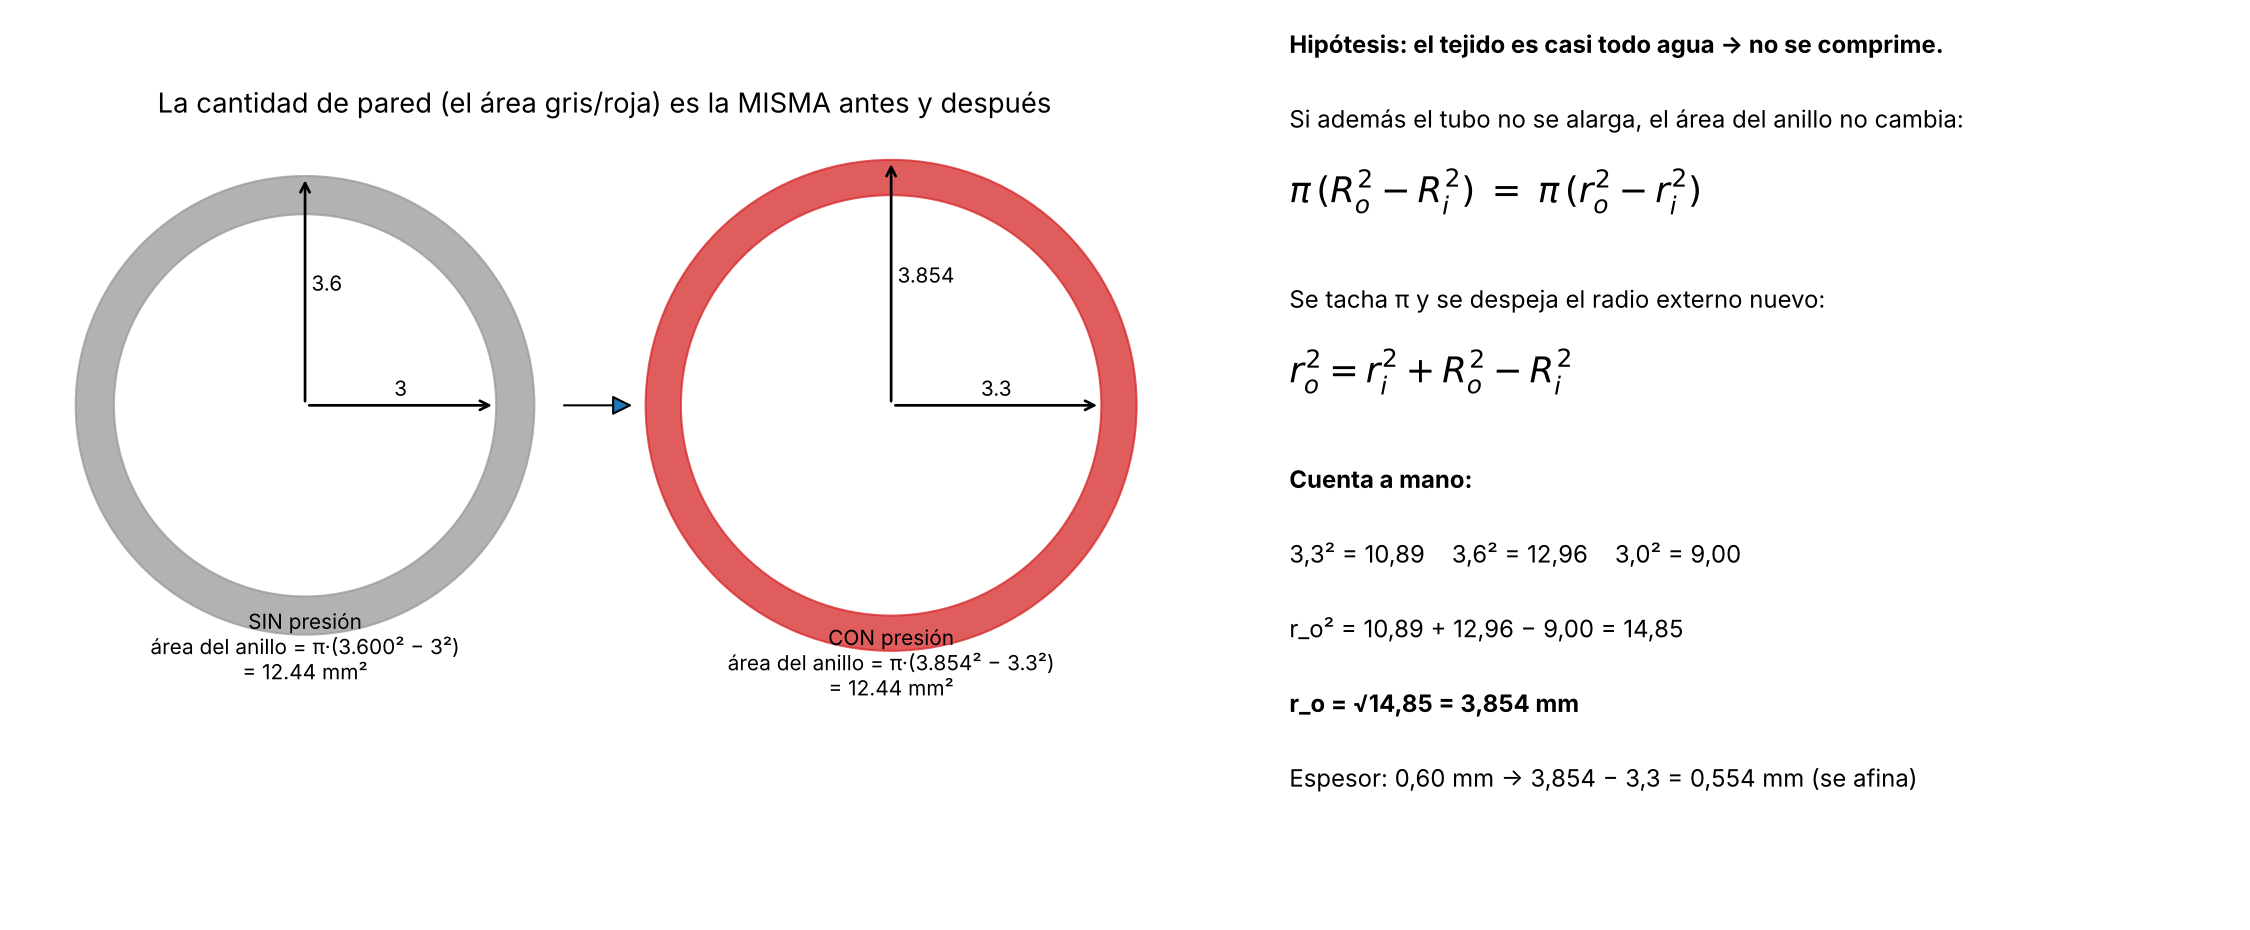
\includegraphics[width=0.9\textwidth]{d5_area_constante.png}
\caption{El área del anillo (gris sin presión, roja con presión) es la misma: $\pi(3{,}6^2-3{,}0^2)=\pi(3{,}854^2-3{,}3^2)=12{,}44$\,mm$^2$.}\end{figure}

\subsection{La pared gruesa como pila de paredes delgadas}
Se corta la pared en rebanadas finas. Cada rebanada es una pared delgada, con su propio estiramiento $\lambda=r_c/R_c$ (en su centro), y aporta $\sigma\,\Delta r/r_c$ (Laplace); la presión es la suma, que en el límite es la integral de la ec.~\eqref{eq:pgruesa}.
\begin{figure}[H]\centering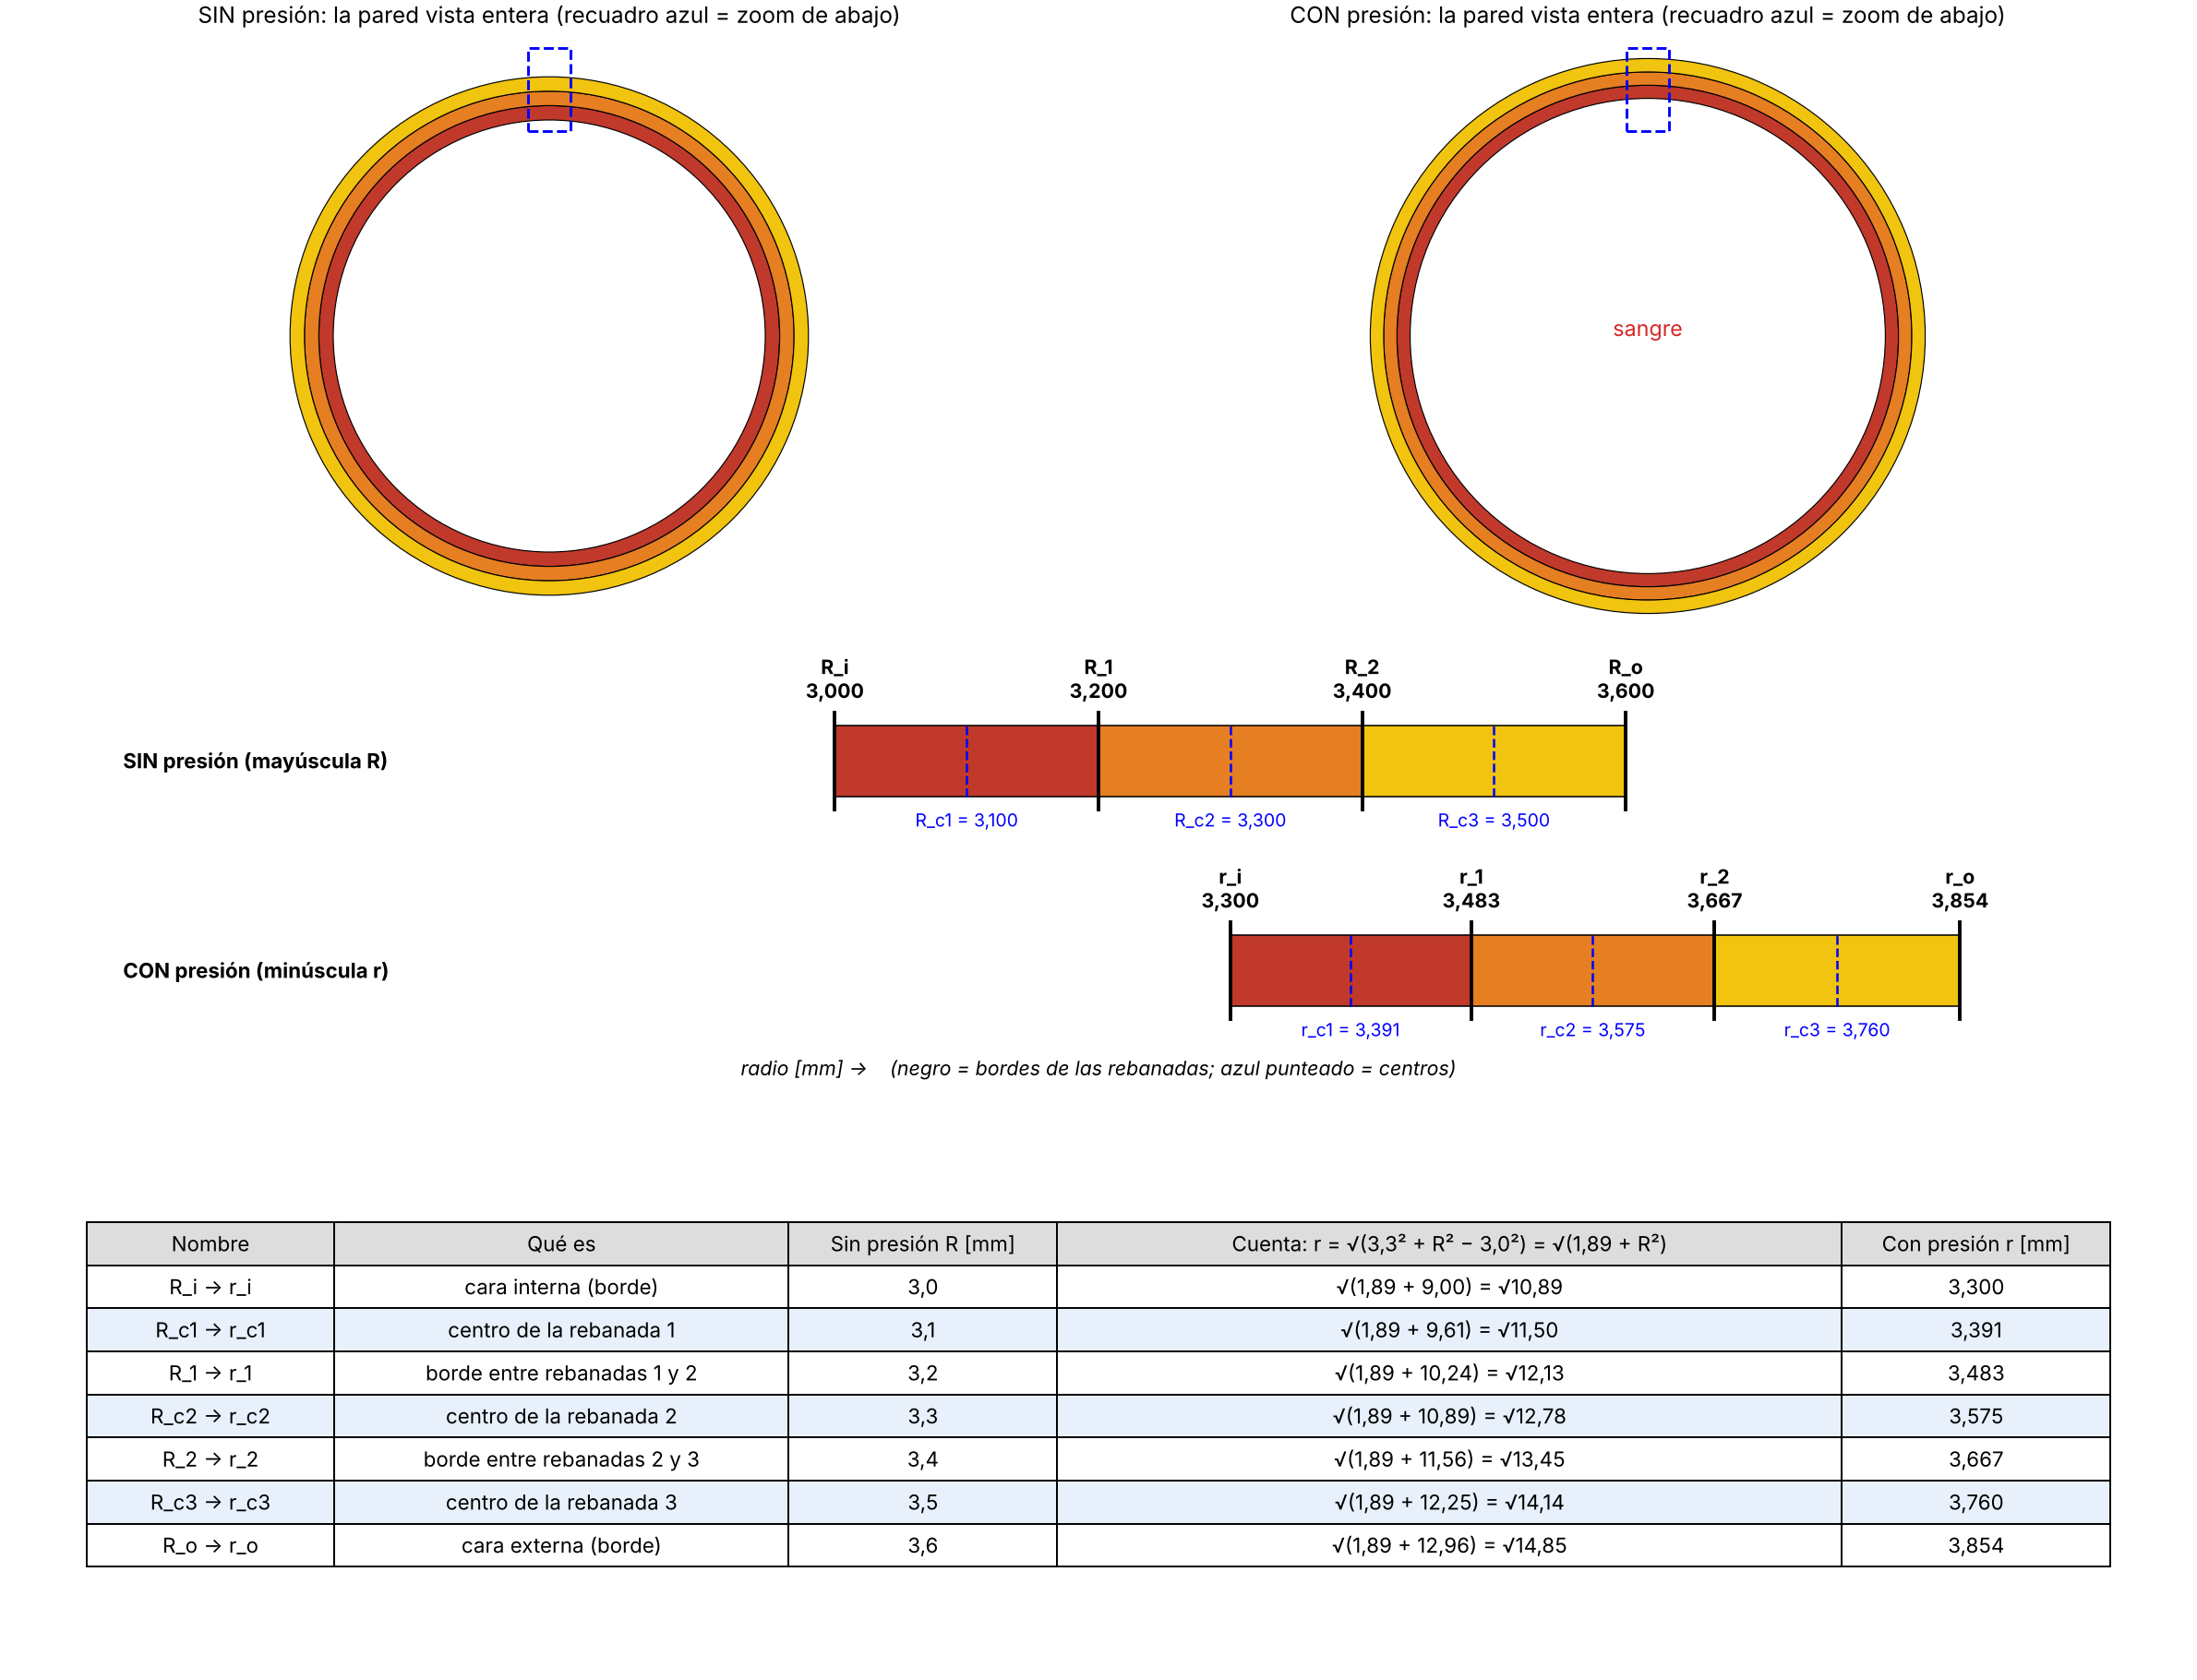
\includegraphics[width=0.9\textwidth]{d15_radios_rebanadas.png}
\caption{El tubo de ejemplo en 3 rebanadas: bordes (negro) y centros (azul), sin presión ($R$) y con presión ($r=\sqrt{1{,}89+R^2}$).}\end{figure}
Con un material sin nudo, $\sigma=1000\,(\lambda-1)$\,kPa:
\begin{center}\small
\begin{tabular}{lccc}\toprule
 & Rebanada 1 (adentro) & Rebanada 2 & Rebanada 3 (afuera)\\\midrule
centro sin presión $R_c$ [mm] & 3,1 & 3,3 & 3,5\\
centro con presión $r_c=\sqrt{1{,}89+R_c^2}$ [mm] & 3,391 & 3,575 & 3,760\\
estiramiento $\lambda=r_c/R_c$ & 1,094 & 1,083 & 1,074\\
tensión $\sigma$ [kPa] & 93,9 & 83,3 & 74,4\\
espesor inflado $\Delta r$ [mm] & 0,183 & 0,185 & 0,186\\
aporte $\sigma\,\Delta r/r_c$ [kPa] & 5,06 & 4,30 & 3,68\\\bottomrule
\end{tabular}
\end{center}
La presión total es $5{,}06+4{,}30+3{,}68=13{,}05$\,kPa (con miles de rebanadas, 13,07). La rebanada de adentro aporta más porque se estira más.
\begin{figure}[H]\centering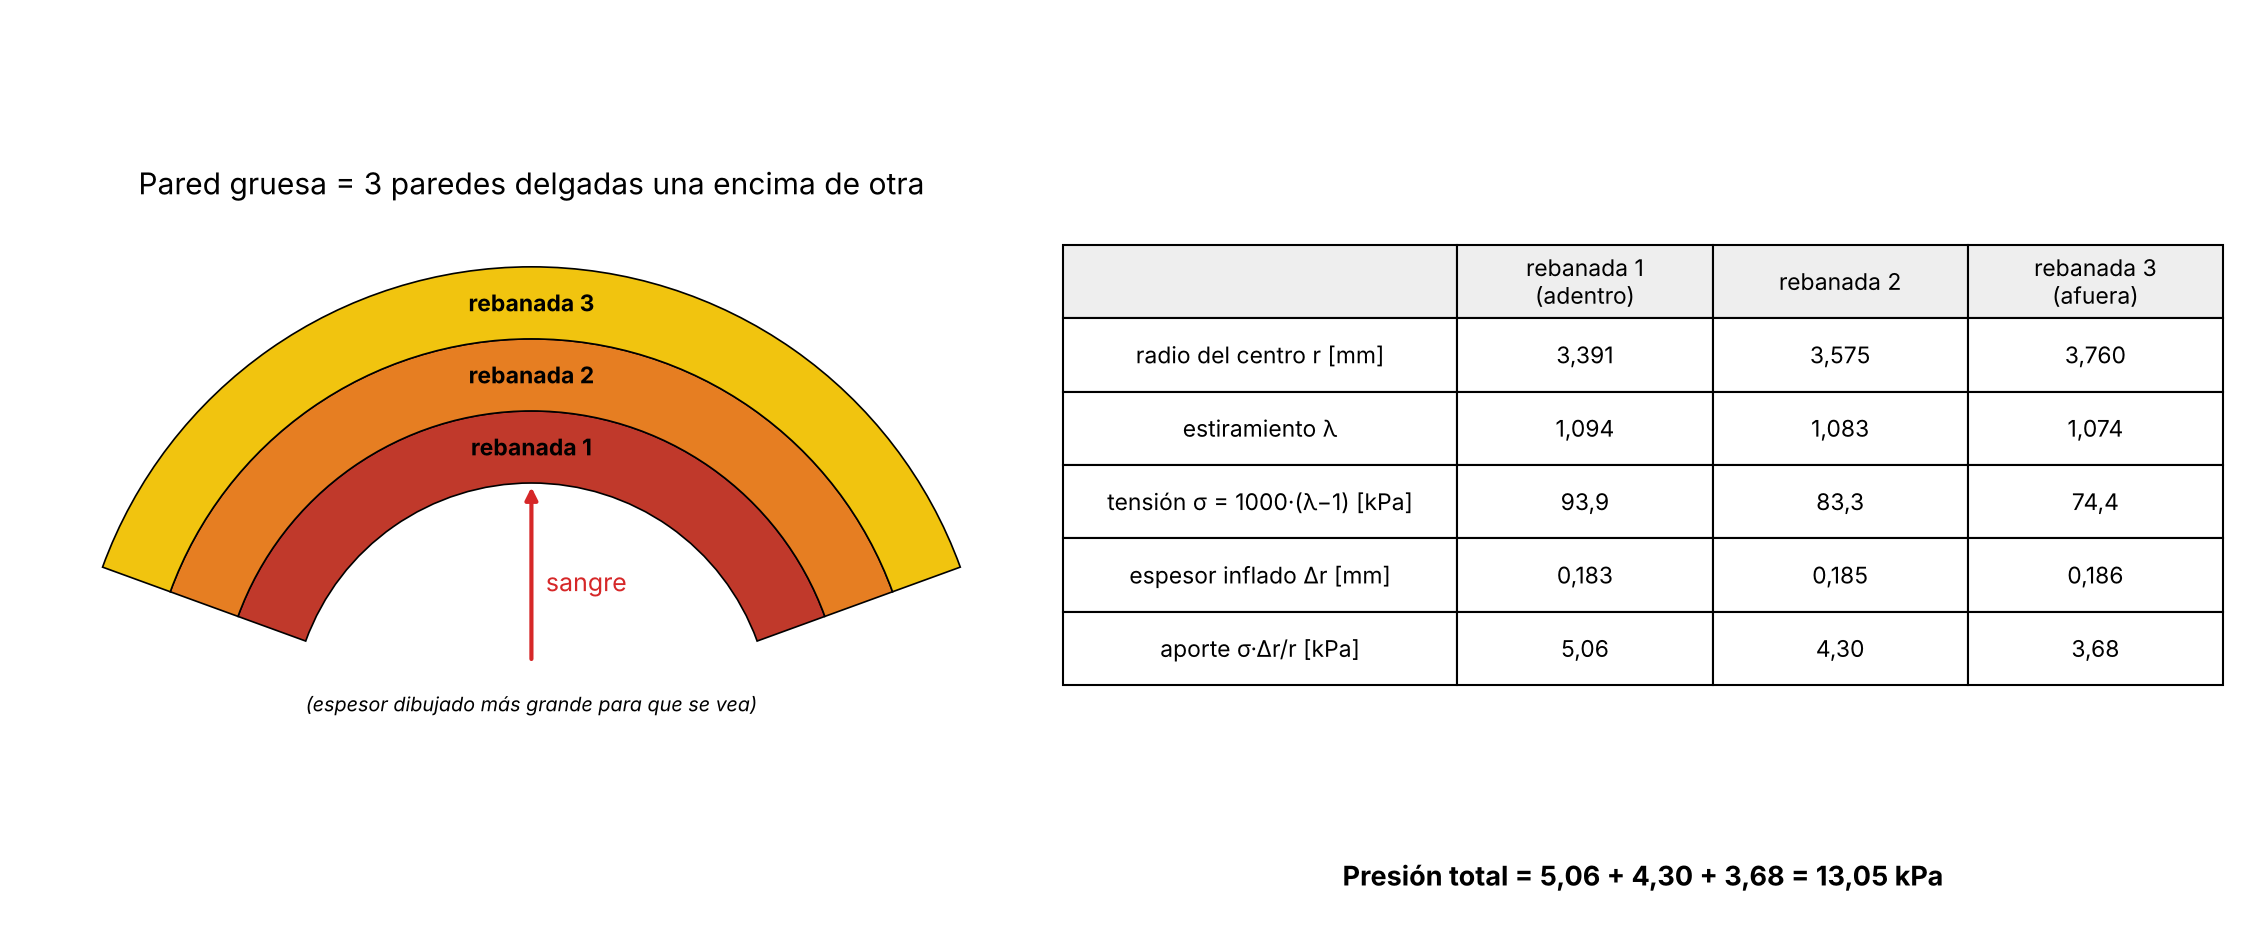
\includegraphics[width=0.55\textwidth]{d13_rebanadas.png}
\caption{Pared gruesa = tres paredes delgadas, una encima de otra.}\end{figure}

\subsection{En pared gruesa importa dónde va cada capa}
Ahora la pared tiene dos materiales con nudo, $\sigma=E\max(0,\lambda-k)$: una capa azul ($k=1{,}02$, $E=400$\,kPa) de 3,0 a 3,3\,mm y una verde ($k=1{,}08$, $E=1500$\,kPa) de 3,3 a 3,6\,mm, cada una cortada en 3 franjas.
\begin{figure}[H]\centering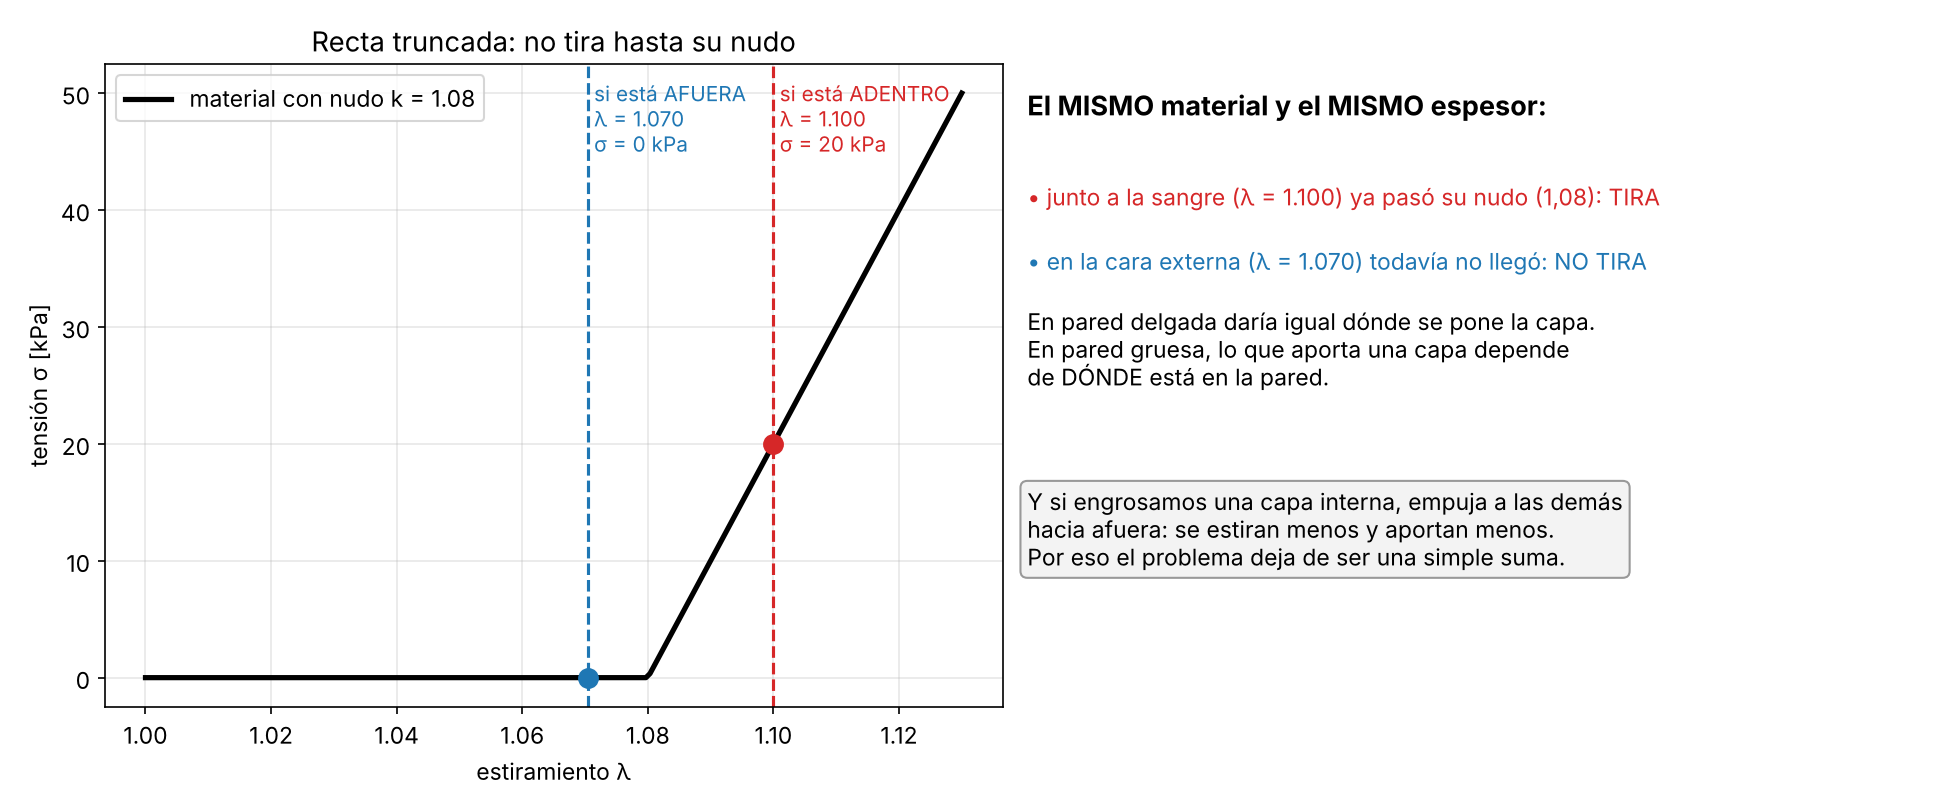
\includegraphics[width=0.9\textwidth]{d3_posicion.png}
\caption{Un material con nudo 1,08 (en el dibujo, $E=1000$\,kPa) tira si está junto a la sangre ($\lambda=1{,}100$: $\sigma=1000\times0{,}020=20$\,kPa) y no tira en la cara externa ($\lambda=1{,}070<1{,}08$: $\sigma=0$). El mismo material y el mismo espesor aportan distinto según dónde estén.}\end{figure}
\begin{figure}[H]\centering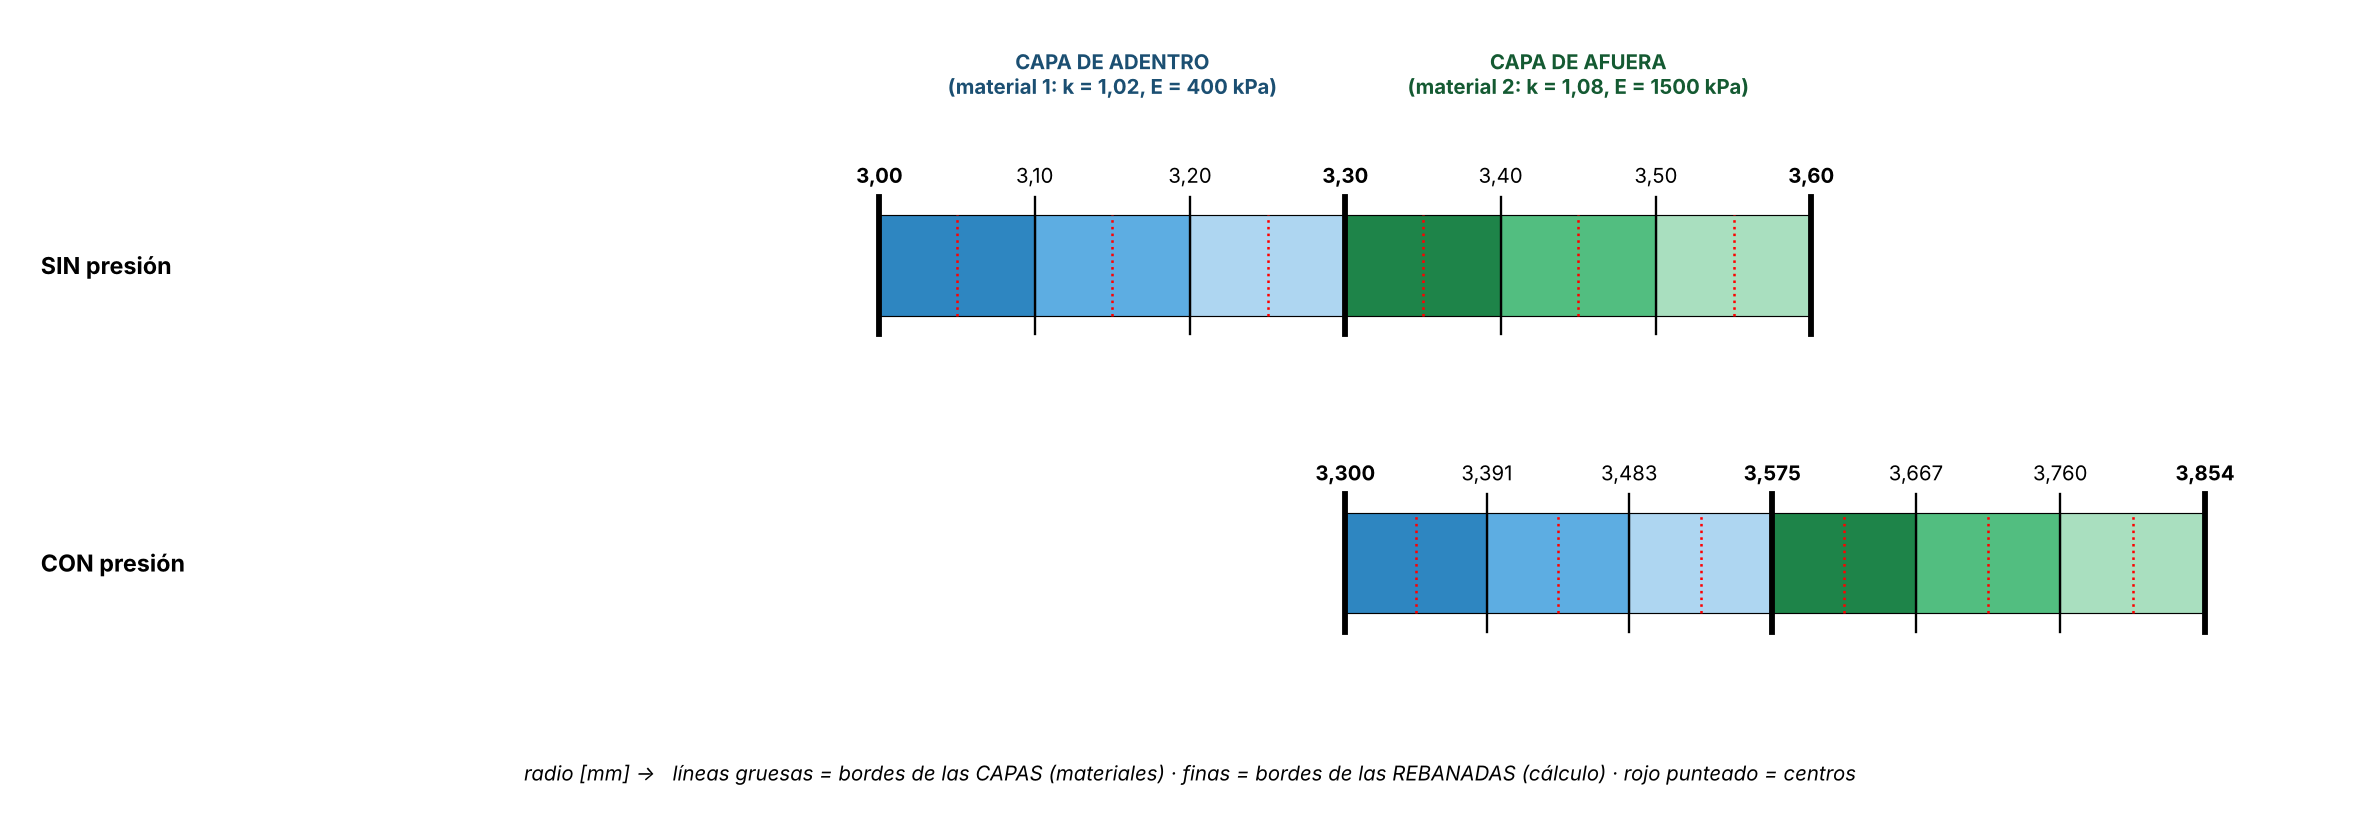
\includegraphics[width=\textwidth]{d16_dos_capas.png}
\caption{Dos capas de 0,3\,mm, sin presión (arriba) y con presión (abajo). La capa azul aporta $0{,}84+0{,}76+0{,}69=2{,}28$\,kPa; de la verde solo tira la primera franja ($\lambda=1{,}081$): 0,04\,kPa.}\end{figure}
Si se cambia solo el espesor de la capa azul, la verde ---que no se tocó--- cambia lo que aporta, porque queda empujada hacia afuera y se estira menos:
\begin{figure}[H]\centering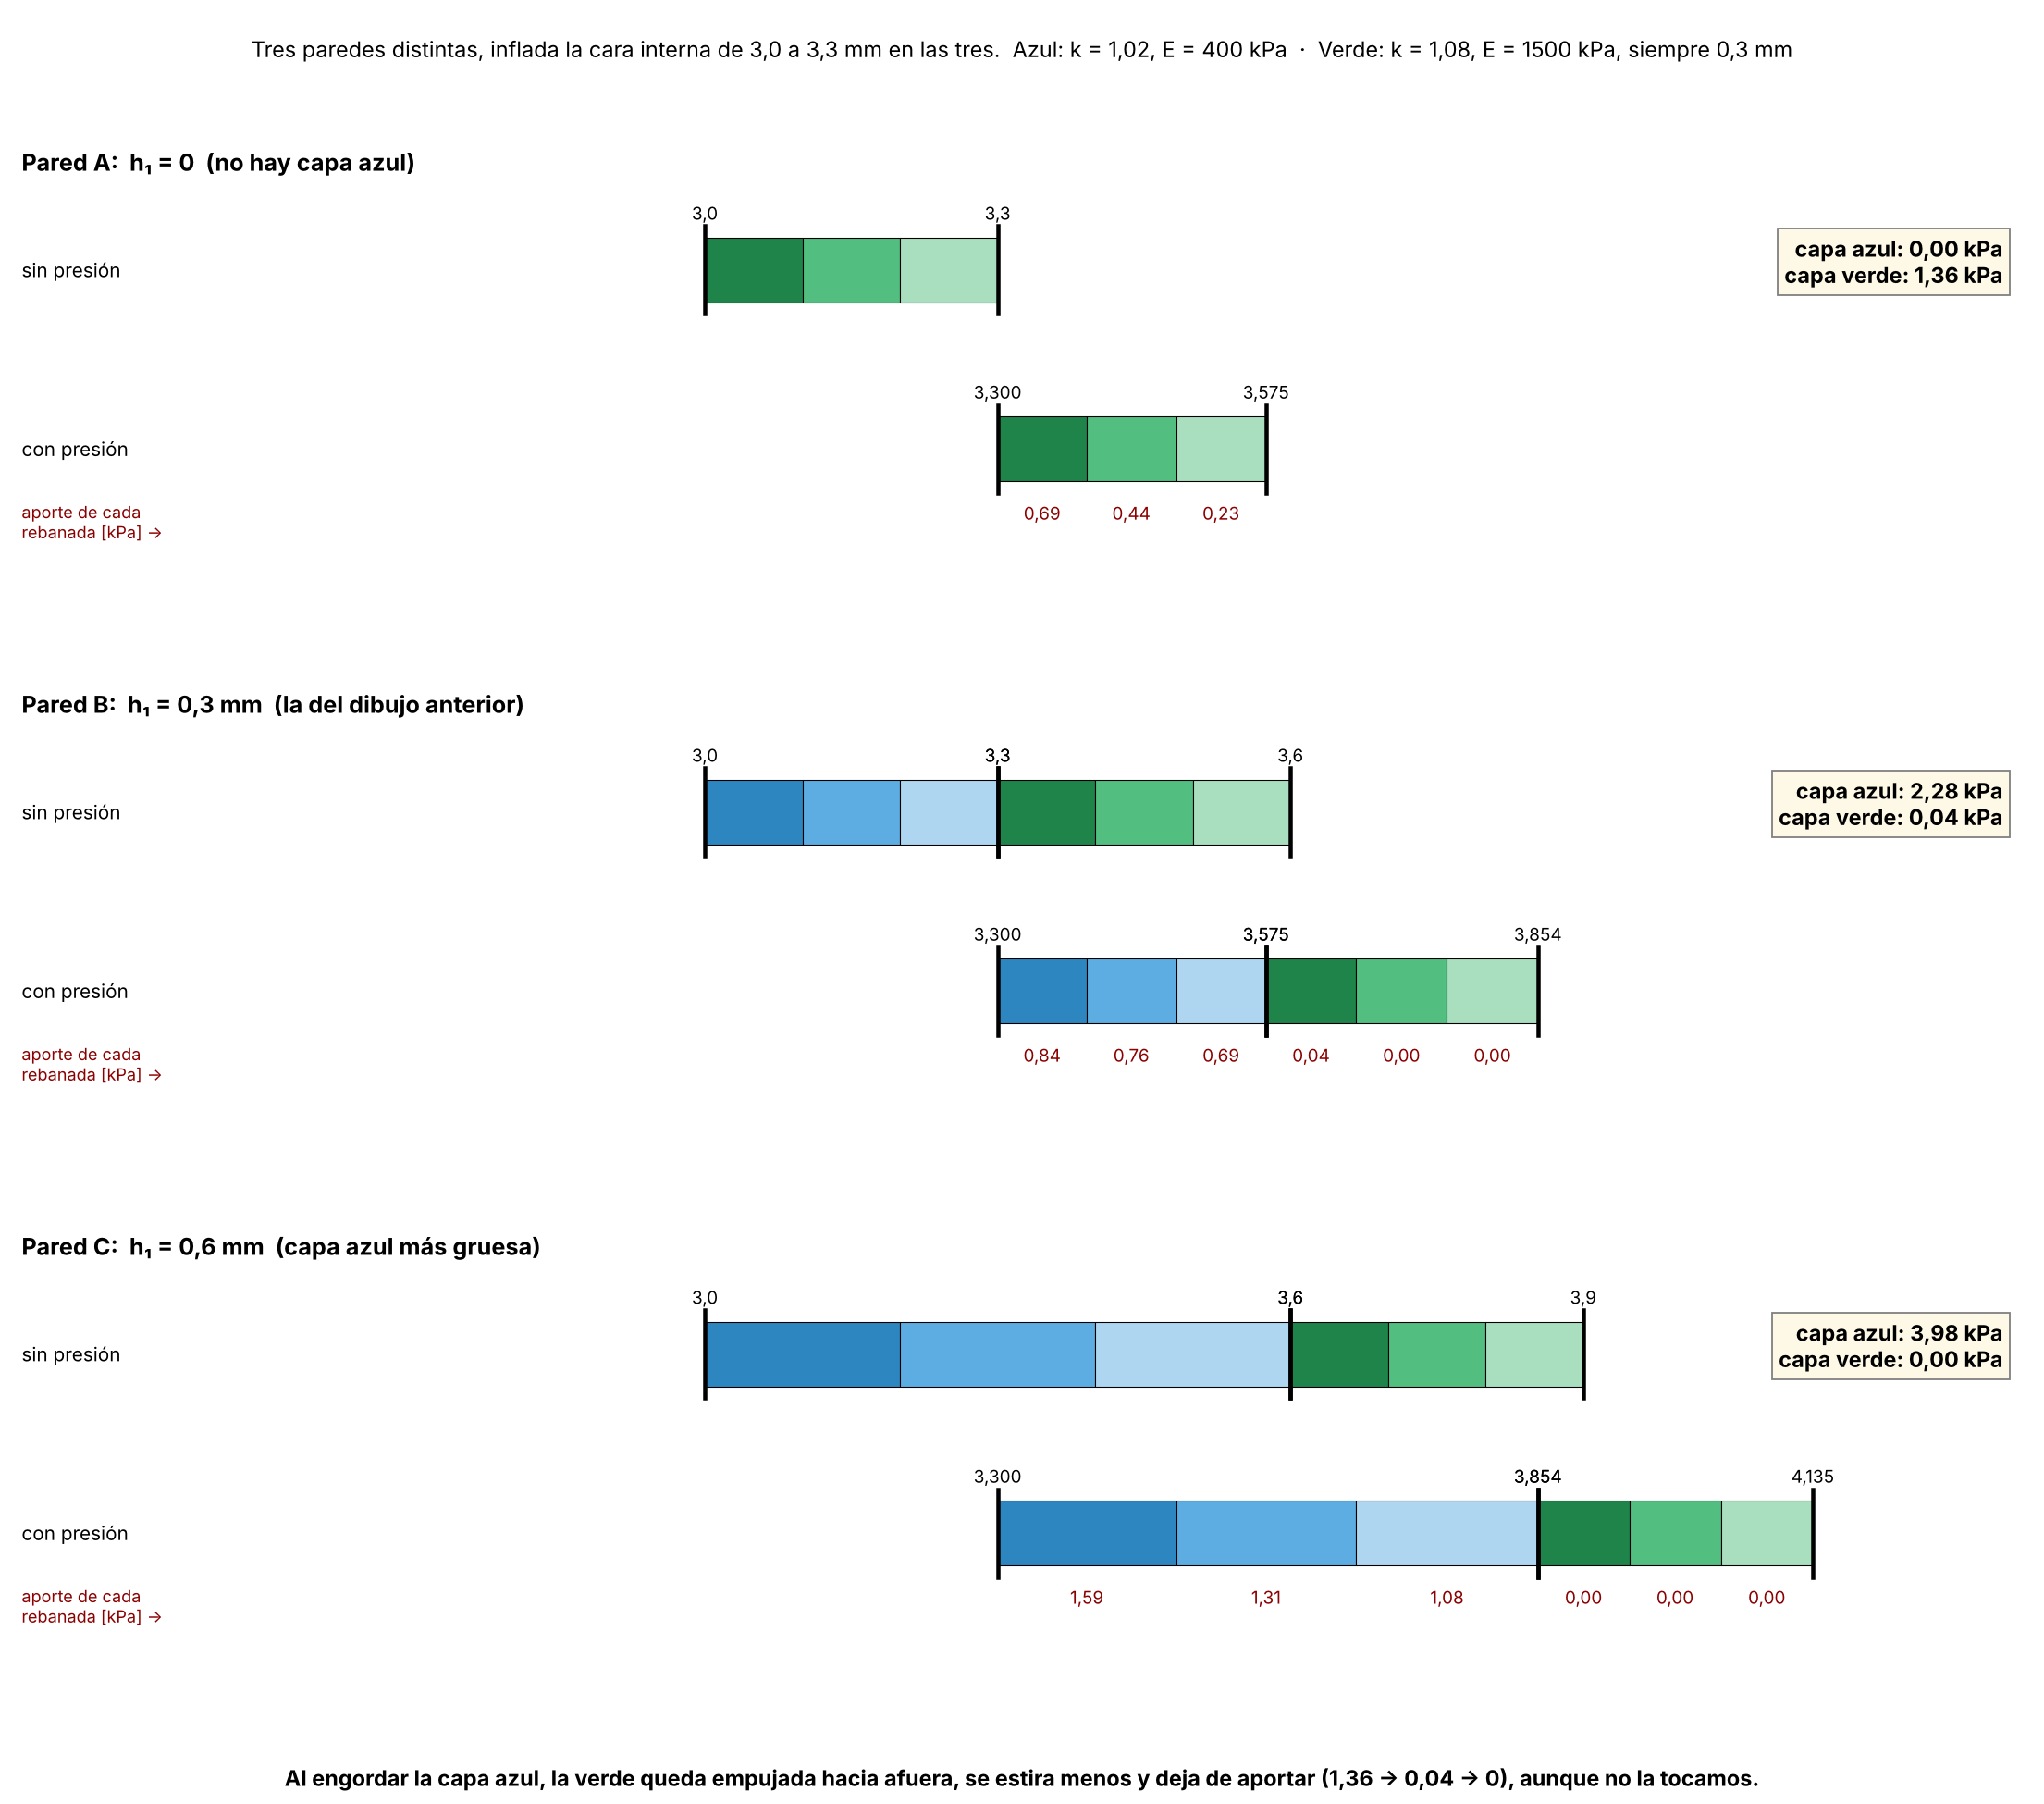
\includegraphics[width=\textwidth]{d17_tres_paredes.png}
\caption{Tres paredes con la misma capa verde de 0,3\,mm y la misma cara interna inflada a 3,3\,mm. Sin capa azul la verde aporta 1,36\,kPa; con 0,3\,mm de azul, 0,04; con 0,6\,mm, nada. Al duplicar la azul su aporte pasa de 2,28 a 3,98\,kPa, que no es el doble: el problema es no lineal en los espesores.}\end{figure}
\begin{figure}[H]\centering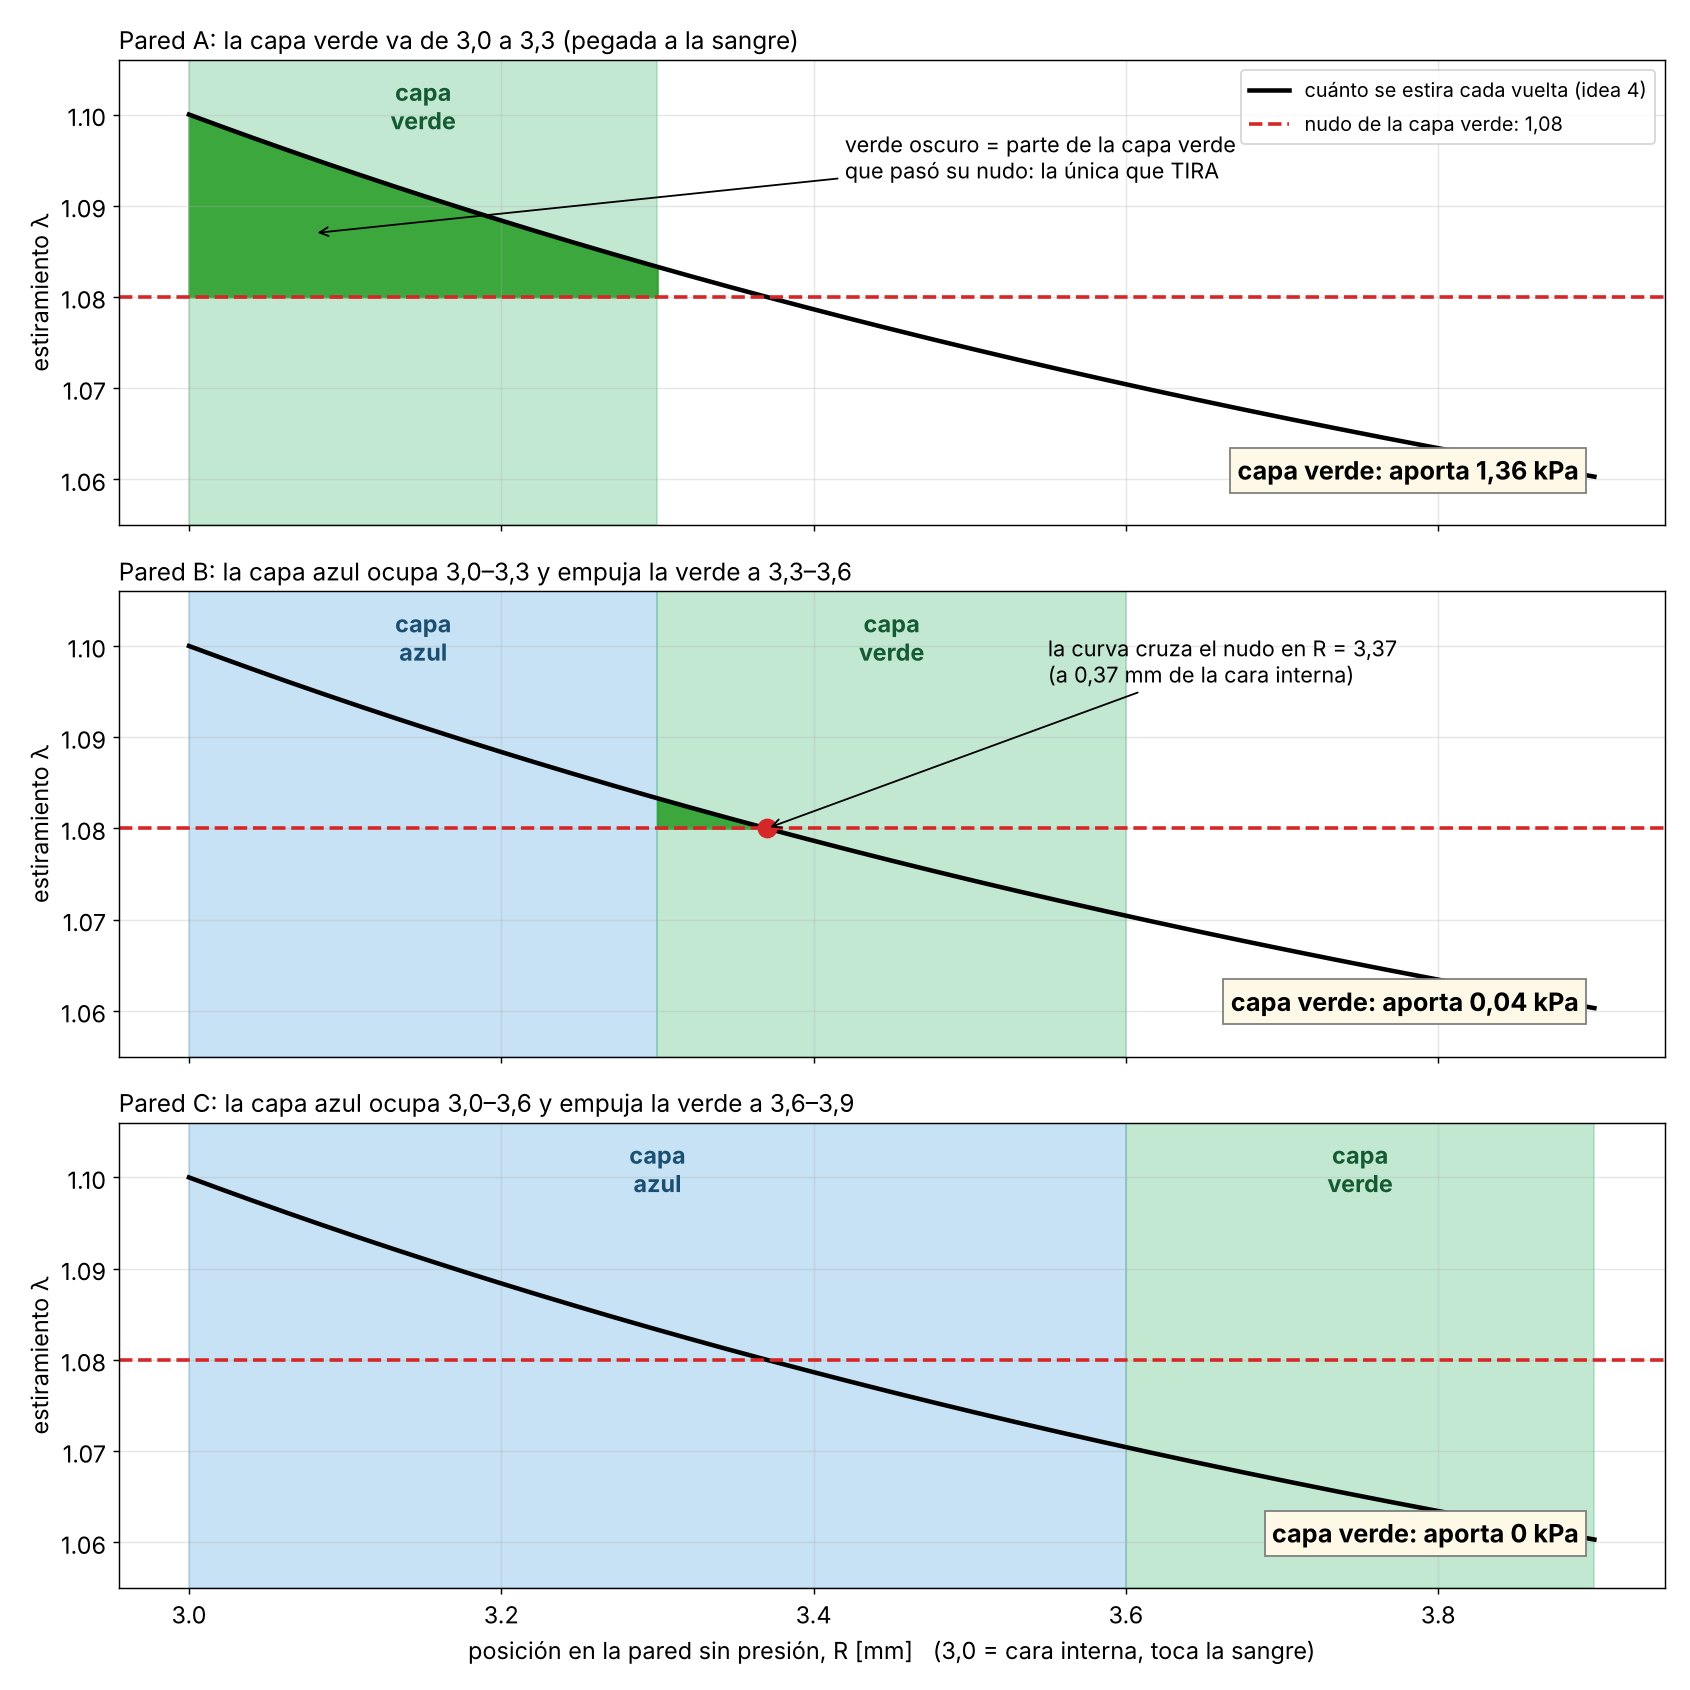
\includegraphics[width=0.85\textwidth]{d18_verde_y_nudo.png}
\caption{Las mismas tres paredes vistas como estiramiento de cada vuelta en función de su radio sin presión (curva negra) y nudo de la capa verde (línea roja). La capa verde solo aporta en la parte de ella que queda por encima de 1,08 (verde oscuro): en A toda su cara interna; en B, una astilla junto a $R=3{,}37$\,mm; en C, nada.}\end{figure}

\subsection{El preestiramiento $\delta$}
$\delta$ corre todos los nudos juntos: el azul pasa a $1{,}02+\delta$ y el verde a $1{,}08+\delta$. Se repite la cuenta de la pared de dos capas (azul de 3,0 a 3,3, verde de 3,3 a 3,6\,mm, cara interna inflada a 3,3\,mm) con tres valores de $\delta$. Los estiramientos de las franjas no cambian (dependen solo de la geometría); cambia desde dónde tira cada material.
\begin{center}\small
\begin{tabular}{lccccc}\toprule
 & & $\lambda$ & \multicolumn{3}{c}{$\sigma$ [kPa]}\\\cmidrule(lr){4-6}
Capa & centro $R$ [mm] & & $\delta=-0{,}03$ & $\delta=0$ & $\delta=+0{,}03$\\\midrule
azul, $\sigma=400\max(0,\lambda-1{,}02-\delta)$ & 3,05 & 1,097 & 42,8 & 30,8 & 18,8\\
 & 3,15 & 1,091 & 40,4 & 28,4 & 16,4\\
 & 3,25 & 1,086 & 38,3 & 26,3 & 14,3\\
verde, $\sigma=1500\max(0,\lambda-1{,}08-\delta)$ & 3,35 & 1,081 & 46,4 & 1,4 & 0\\
 & 3,45 & 1,076 & 39,7 & 0 & 0\\
 & 3,55 & 1,072 & 33,6 & 0 & 0\\\midrule
\multicolumn{3}{l}{aporte de la capa azul [kPa]} & 3,24 & 2,28 & 1,32\\
\multicolumn{3}{l}{aporte de la capa verde [kPa]} & 3,00 & 0,04 & 0\\
\multicolumn{3}{l}{presión total [kPa]} & 6,25 & 2,33 & 1,32\\\bottomrule
\end{tabular}
\end{center}
Ejemplo de verificación: primera franja azul con $\delta=-0{,}03$: el nudo es $1{,}02-0{,}03=0{,}99$ y $\sigma=400\times(1{,}097-0{,}99)=42{,}8$\,kPa; su aporte es $42{,}8\times0{,}091/3{,}346=1{,}16$\,kPa. Con $\delta=-0{,}03$ toda la capa verde pasa su nudo (1,05) y aporta tanto como la azul; con $\delta=+0{,}03$ el nudo verde sube a 1,11 y la capa verde no trabaja. Así, $\delta$ elige \emph{qué materiales están activos} en el tramo de estiramiento de cada sujeto: un sujeto blando, que se estira mucho, necesita nudos más a la derecha ($\delta>0$), y uno rígido, más a la izquierda ($\delta<0$). Sin $\delta$, cada sujeto vería solo uno o dos de los nudos de la base.
\begin{figure}[H]\centering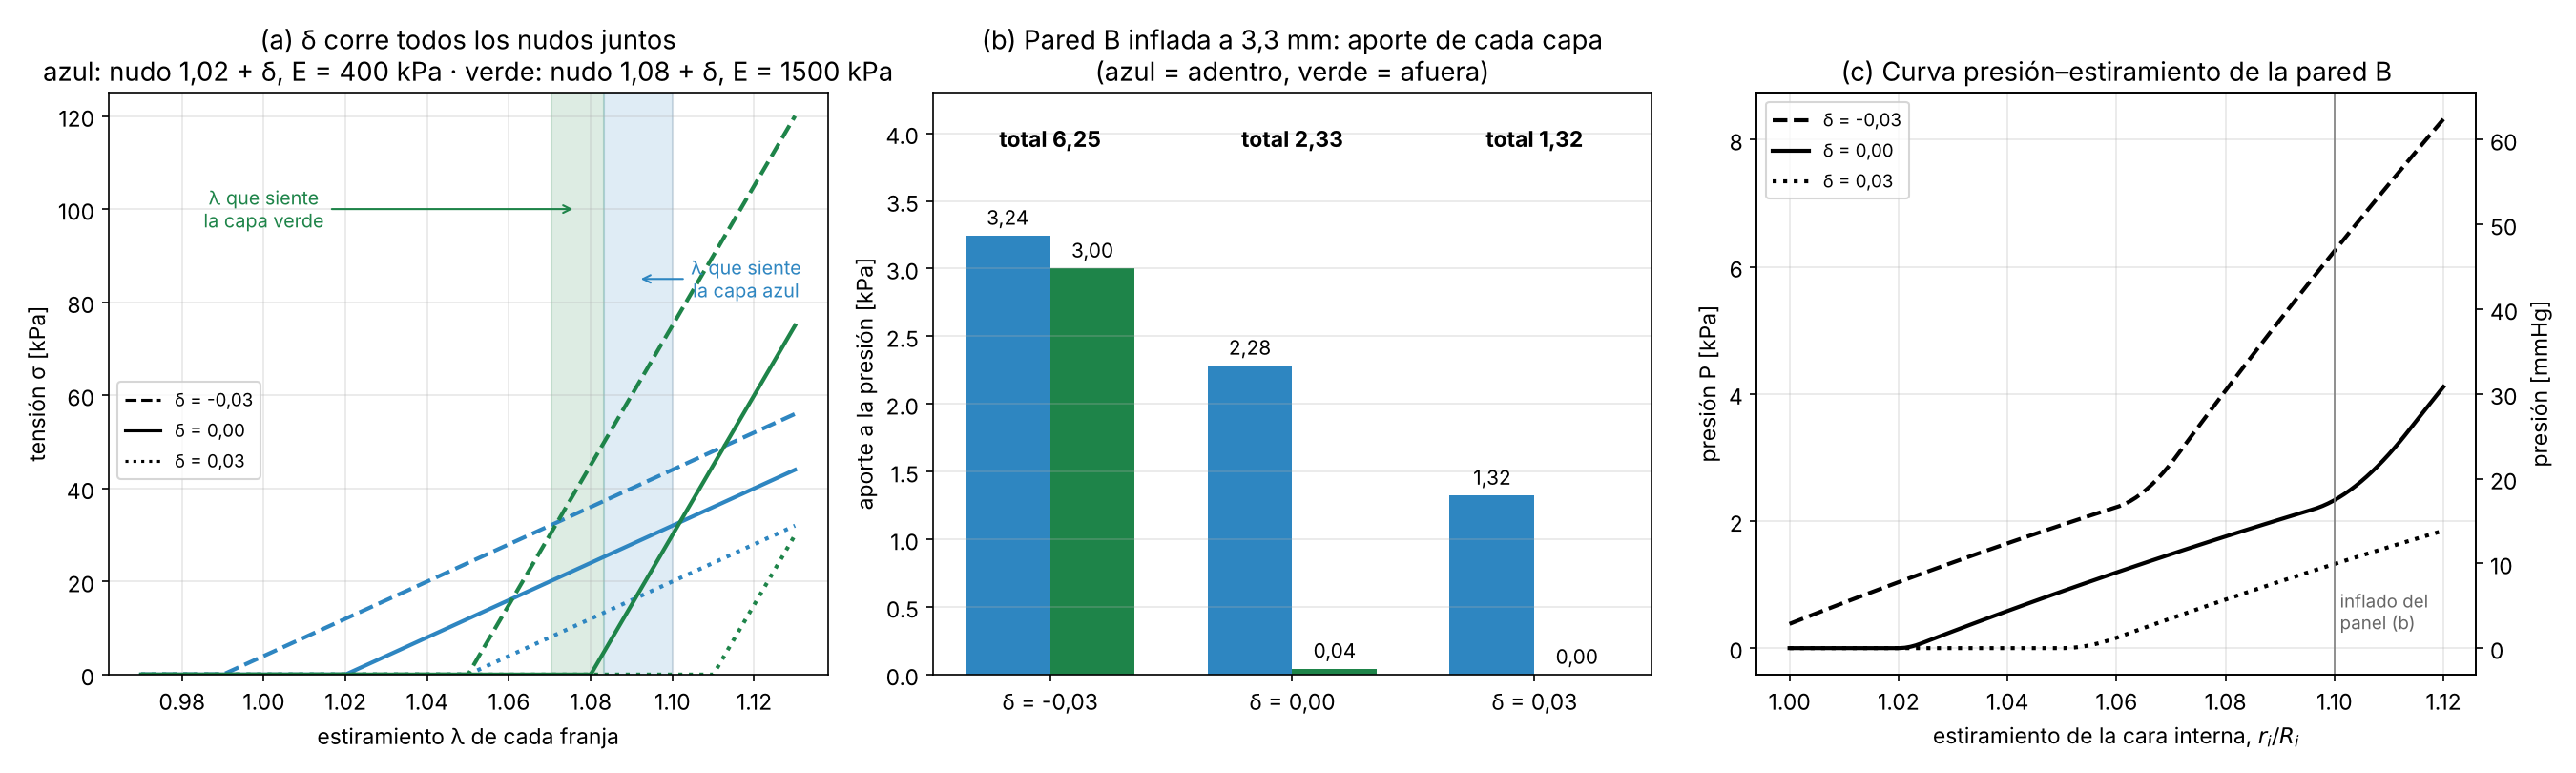
\includegraphics[width=\textwidth]{d19_delta.png}
\caption{Efecto de $\delta$ en la pared de dos capas. (a) Ley de cada material para $\delta=-0{,}03$, 0 y $+0{,}03$; las franjas sombreadas son los estiramientos que siente cada capa con la cara interna en 3,3\,mm. (b) Aporte de cada capa a la presión en ese estado. (c) Curva presión--estiramiento de la cara interna (eje derecho en mmHg): $\delta$ corre el punto donde engancha cada capa y cambia la forma de la curva. Los valores son de un ejemplo de juguete (capas de 0,3\,mm y módulos bajos), no de un diseño.}\end{figure}

\clearpage
\section{Detalles del cálculo a nivel del tubo}\label{sec:calculo}
\subsection{Pared delgada: Laplace y Urquiza}
Urquiza~\cite{urquiza} (ec.~3.13 de su tesis) escribe el equilibrio de pared delgada con el radio y el espesor \emph{instantáneos}, $(P_i-P_a)\,R=\sigma\,h$. Tomando como $R$ el radio medio deformado, $\bar r=r_i+h/2$, y llamando $u=1+h/r_i$,
\begin{equation}\label{eq:urquiza}
P=\frac{\sigma\,h}{r_i+h/2}=\sigma\,\frac{2\,(u-1)}{u+1}.
\end{equation}
Para una pared homogénea con tensión uniforme, \eqref{eq:equil} da exactamente $P=\sigma\ln u$, y $2(u-1)/(u+1)$ es la aproximación de Padé [1/1] de $\ln u$: con $h/r_i\le0{,}2$ el error es menor que 0,3\,\%, mientras que Laplace con el radio interno, $P=\sigma\,(u-1)$, sobreestima la presión hasta en un 10\,\%. Llamamos \emph{ley de Urquiza} a \eqref{eq:urquiza} aplicada al injerto multicapa con un único estiramiento, el del radio medio: $P=\sum_j\sigma_j(\bar\lambda)\,h_j/\bar r$, con $\bar\lambda=\bar r/\bar R$. Sigue siendo lineal en los espesores. En la Tabla~\ref{tab:laplace} Laplace usa el radio y el espesor sin deformar.

\textbf{Juego de nudos de la comparación.} La Tabla~\ref{tab:laplace} se calculó sobre curvas de presión en $\lambda$ de 1,02 a 1,16, con espesores reales y un juego de nudos ajustado a esas curvas (distinto del de la Tabla~\ref{tab:bases}): 0,8271; 1,0219; 1,0867; 1,1197; 1,1391; 1,1531, con módulos 0,18; 1,33; 4,86; 2,72; 12,94; 6,35\,MPa. La Tabla~\ref{tab:laplace3} da los diseños de la Fig.~\ref{fig:laplace}. Con la ventana de presión y la base adoptadas, el diseño lineal de pared delgada tampoco cumple en ningún sujeto (mediana 27,3\,\% con 6 materiales y 29,9\,\% con 5).

\begin{table}[H]\centering\small
\caption{Diseños de la Fig.~\ref{fig:laplace} (6 materiales): espesor de la capa de cada material $h_j$ [µm] (capa 1 junto a la sangre; 0: no se usa), pared total [µm] y errores contra la curva de presión de la arteria, $E_{\mathrm{rms}}$ y $e_{\max}$ [\% del rango]. ``Laplace, en su modelo'' y ``Laplace, injerto real'' son el mismo diseño evaluado con dos modelos.}\label{tab:laplace3}
\resizebox{\textwidth}{!}{%
\begin{tabular}{llccccccccc}\toprule
Curva & Diseño y evaluación & $h_1$ & $h_2$ & $h_3$ & $h_4$ & $h_5$ & $h_6$ & pared & $E_{\mathrm{rms}}$ & $e_{\max}$\\\midrule
$y_1$ & Laplace, en su modelo & 25 & 153 & 0 & 56 & 0 & 0 & 233 & 1,47 & 2,01\\
 & Laplace, injerto real & 25 & 153 & 0 & 56 & 0 & 0 & 233 & 1,98 & 3,36\\
 & Urquiza, injerto real & 25 & 153 & 0 & 56 & 0 & 0 & 233 & 2,01 & 3,29\\
 & Pared gruesa, injerto real & 25 & 130 & 25 & 0 & 0 & 29 & 210 & 1,47 & 2,46\\
\addlinespace
Media HT & Laplace, en su modelo & 235 & 203 & 59 & 205 & 67 & 136 & 905 & 0,41 & 0,76\\
 & Laplace, injerto real & 235 & 203 & 59 & 205 & 67 & 136 & 905 & 5,14 & 16,79\\
 & Urquiza, injerto real & 250 & 196 & 62 & 204 & 66 & 132 & 909 & 5,40 & 16,79\\
 & Pared gruesa, injerto real & 129 & 158 & 48 & 218 & 0 & 467 & 1020 & 0,34 & 0,60\\
\addlinespace
$y_2$ & Laplace, en su modelo & 449 & 229 & 139 & 461 & 193 & 30 & 1500 & 1,08 & 1,73\\
 & Laplace, injerto real & 449 & 229 & 139 & 461 & 193 & 30 & 1500 & 7,95 & 24,69\\
 & Urquiza, injerto real & 453 & 241 & 141 & 454 & 187 & 25 & 1500 & 8,24 & 24,30\\
 & Pared gruesa, injerto real & 203 & 122 & 67 & 626 & 206 & 277 & 1500 & 0,61 & 0,87\\
\bottomrule
\end{tabular}}
\end{table}

\subsection{El modelo del injerto}
El injerto es un tubo cerrado, incompresible y en deformación plana, centrado en $R_{\mathrm{ref}}=3{,}421$\,mm (mediana de $\Theta_0R_m/\pi$ de los 41 sujetos). Las capas van por nudo creciente de adentro hacia afuera (el orden inverso duplica o triplica el error). Con pared incompresible y sin alargamiento, el área entre la cara interna y una fibra que estaba en el radio $R$ se conserva:
\begin{equation}\label{eq:incomp}
r^2-r_i^2=R^2-R_i^2,\qquad\lambda(r)=\frac{r}{R}.
\end{equation}
Cada capa engancha cuando la pared media llega a $k_j+\delta$; su enganche local $\kappa_j$ es el estiramiento del centro de la capa en ese momento, por \eqref{eq:incomp}. En fabricación, $\kappa_j$ es el rizado de las fibras de esa capa. Los módulos se calibran para que el sujeto de entrenamiento que más necesita de cada material use 0,2\,mm de él, y luego se multiplican por los factores de la Sección~\ref{sec:aplicacion} (6 materiales: de 452 a 7449\,kPa). La búsqueda se limita a $|\delta|\le0{,}25$, es decir $-0{,}25\le\delta\le0{,}25$: más ancho que todo el tramo de estiramiento que recorre un sujeto (0,21), para que ningún sujeto quede fuera por la cota; en los diseños, $\delta$ queda lejos de ella.

La presión \eqref{eq:pgruesa} se integra en cada capa con cuadratura de Gauss--Legendre de 8 nodos~\cite{davis} en 651 valores de $\lambda$ entre 0,80 y 1,45, y se invierte por interpolación lineal para obtener $\lambda_{\mathrm{inj}}(P_k;\theta)$, con $\theta=(h_1,\dots,h_N,\delta)$. La función $\theta\mapsto\lambda_{\mathrm{inj}}$ es no lineal: los espesores fijan los límites de integración y los enganches, y $\delta$ entra dentro del $\max(0,\cdot)$. Con láminas enteras, el problema es \textbf{no lineal entero mixto}. La métrica es \eqref{eq:emax} sobre $\lambda(P_k)$. Una evaluación del modelo tarda 0,45\,ms.

\subsection{Los algoritmos de los tres pasos}
\begin{table}[H]\centering\small
\caption{Bloques de cálculo a nivel del tubo. ``Lineal'' se refiere a la dependencia del modelo respecto de las incógnitas.}\label{tab:bloques}
\resizebox{\textwidth}{!}{%
\begin{tabular}{>{\raggedright\arraybackslash}p{3.0cm}>{\raggedright\arraybackslash}p{2.2cm}>{\raggedright\arraybackslash}p{1.6cm}>{\raggedright\arraybackslash}p{5.0cm}>{\raggedright\arraybackslash}p{4.1cm}}\toprule
Bloque & Variables & ¿Lineal? & Algoritmo & Implementación\\\midrule
Paso 1: MCO lineal (pared delgada) & reales & sí, con $\delta$ fijo & mínimos cuadrados por SVD; $\delta$ por grilla y Brent & \texttt{numpy.linalg.lstsq}~\cite{numpy}; \texttt{minimize\_scalar}~\cite{brent,scipy}\\
Paso 2: MCO no lineal (pared gruesa) & reales & no & región de confianza reflexiva con cotas (TRF) & \texttt{scipy.optimize.least\_squares}~\cite{branch,scipy}\\
Paso 3: minimax entero (pared gruesa) & láminas enteras, $\delta$ real & no & enumeración piso/techo, $\delta$ por Brent acotado, búsqueda local & propio; \texttt{minimize\_scalar}~\cite{brent}\\
Red en cadena & láminas enteras, $\delta$ real & --- (una evaluación) & red con salida ordinal & TensorFlow/Keras~\cite{tf}\\\bottomrule
\end{tabular}}
\end{table}

\paragraph{Paso 1 · MCO lineal de pared delgada.} Con la ley de Laplace y $\delta$ fijo, la presión es lineal en $c_j=E_jh_j/R_{\mathrm{ref}}$: $P_k\approx\sum_jc_j\max(0,y_k-k_j-\delta)$. Para cada $\delta$ de una grilla de 101 valores se resuelve por mínimos cuadrados; el residuo en presión se pasa a $\lambda$ con la pendiente local de la curva; el mejor $\delta$ se refina por Brent~\cite{brent} y $h_j=c_jR_{\mathrm{ref}}/E_j$, que el paso 2 lleva dentro de sus cotas.

\paragraph{Paso 2 · MCO no lineal de pared gruesa.} Minimiza $\sum_k\bigl((\lambda_{\mathrm{inj}}(P_k;\theta)-y_k)/\Delta\bigr)^2$ con las cotas $0\le h_j\le0{,}5$\,mm y $|\delta|\le0{,}25$, por el método de región de confianza reflexiva (\emph{Trust Region Reflective}, TRF)~\cite{branch}. En cada iteración calcula el jacobiano de los residuos por diferencias finitas, aproxima el problema por su modelo cuadrático de Gauss--Newton y toma el paso que lo minimiza dentro de una \emph{región de confianza}, un entorno donde el modelo es creíble; agranda la región si el paso funcionó y la achica si no, y refleja hacia adentro los pasos que cruzan una cota. Tolerancias $10^{-10}$, a lo sumo 300 evaluaciones. Encuentra un mínimo \emph{local}: el resultado depende del punto de partida.

\paragraph{Paso 3 · Minimax entero.} A partir del diseño real $\theta^\star$ del paso 2 y de su curva $\tilde y$: (1) $n_j\in\{\lfloor h_j^\star/e\rfloor,\lceil h_j^\star/e\rceil\}$, sin pasar de 20; se evalúan las $2^N$ combinaciones por $e_{\max}$ contra $\tilde y$; (2) para las 8 mejores se reajusta $\delta$ en $\pm0{,}03$ por Brent acotado; (3) búsqueda local~\cite{aarts}: vecinos que suman o restan una lámina a un material o pasan una lámina de uno a otro, sin salir de 0 a 20, aceptando el mejor si baja el peor error, hasta 20 veces. Es una heurística: no garantiza el óptimo entero global. Partir de una solución real es la estrategia habitual en problemas no lineales enteros, y es razonable porque un diseño tiene unas 50 láminas y una lámina mueve poco la curva.

\paragraph{Distancia al óptimo entero.} Con los módulos sin recalibrar y sin tope de láminas, en los 41 sujetos se recorrieron \emph{todas} las combinaciones de láminas a $\pm2$ de las del paso 2 (hasta $5^6=15\,625$), cada una con $\delta$ en una grilla de 13 valores y refinado por Brent en las 200 mejores. La búsqueda exhaustiva dio el mismo diseño que el paso 3 en 24 de los 41 sujetos (6 materiales) y en 34 (5 materiales); donde mejoró, el peor punto bajó a lo sumo 0,44 puntos, sin cambiar cuántos sujetos cumplen. La heurística queda a pocas décimas del óptimo en esa vecindad, en 0,5\,s en lugar de 2\,min por sujeto.

\paragraph{Contra qué curva elegir las láminas.} Si el paso 3 eligiera las láminas contra la curva tal como viene medida, perseguiría el peor punto, que con ruido es un salto del ruido (Fig.~\ref{fig:suave}). Contra la curva del paso 2 ese salto no está.

\begin{figure}[H]\centering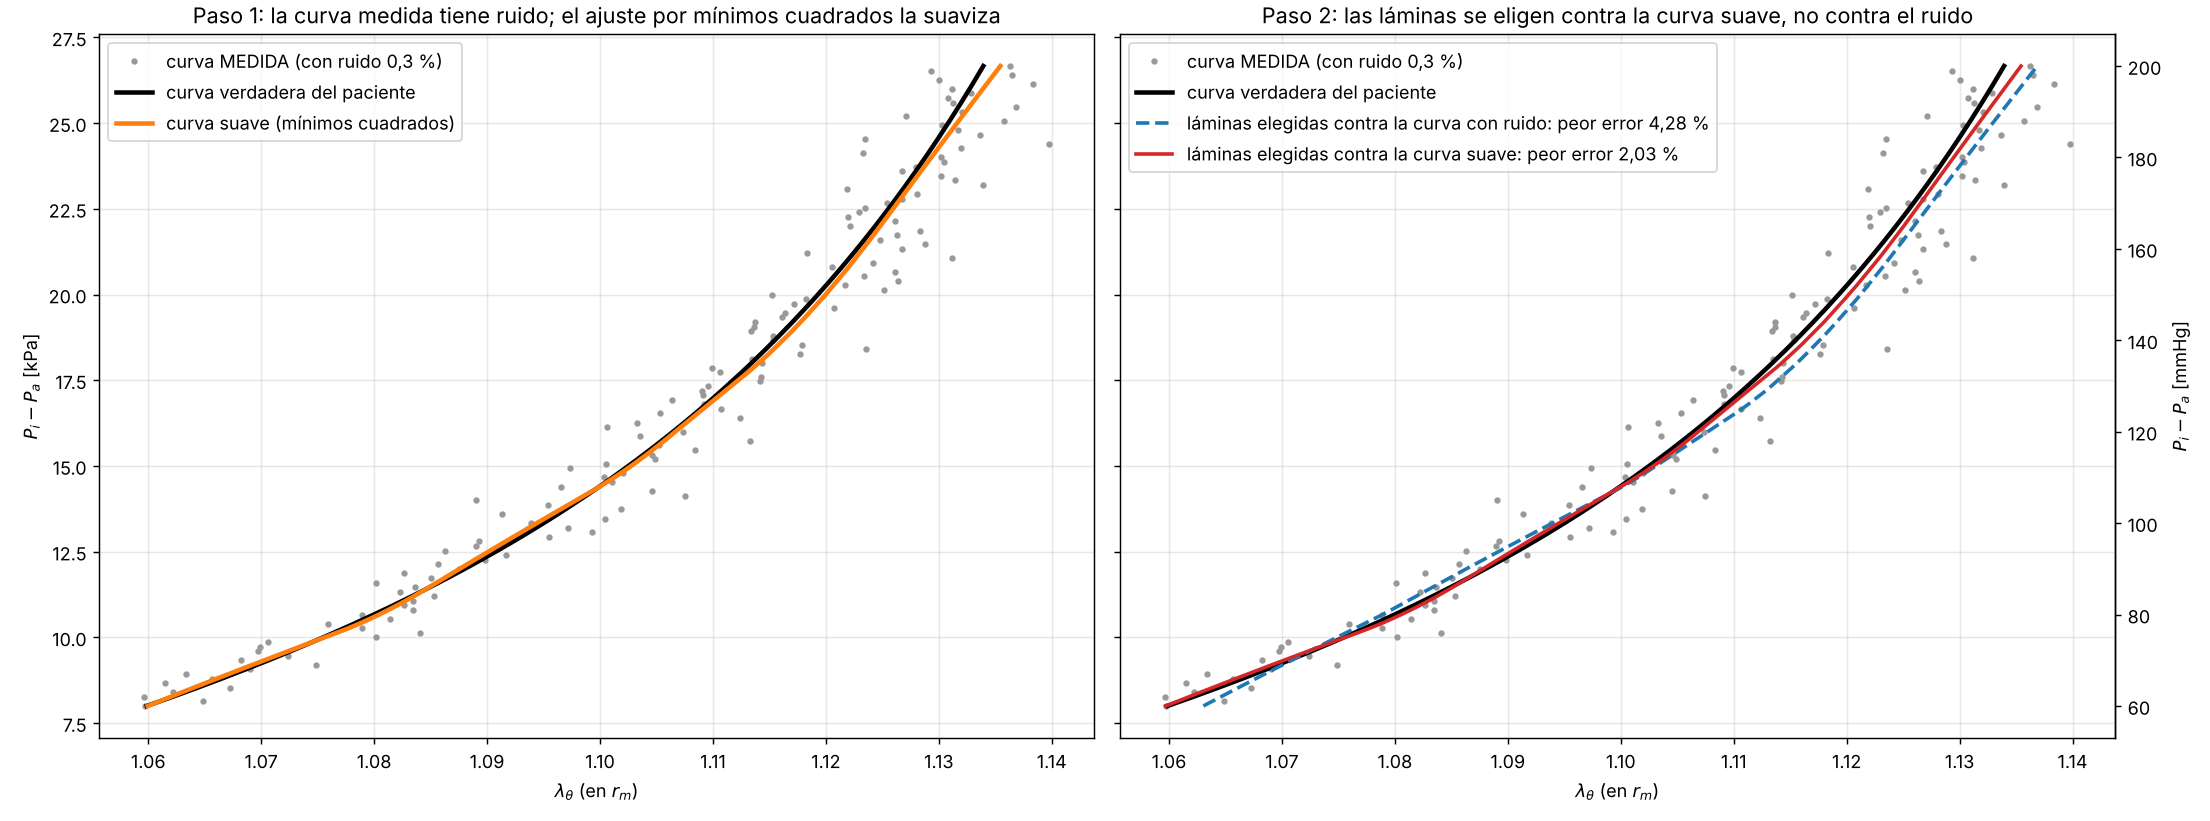
\includegraphics[width=\textwidth]{suavizado_sin_titulo.png}
\caption{Sujeto NT11, 6 materiales, ruido de 0,3\,\% (módulos sin recalibrar). Izquierda: la curva ajustada por el paso 2 (naranja) pasa por el medio de la medida (gris). Derecha: láminas elegidas contra la curva medida ($e_{\max}=4{,}28$\,\%) y contra la ajustada (2,03\,\%), ambas evaluadas contra la verdadera.}\label{fig:suave}\end{figure}

\paragraph{Curvas medidas.} Se simulan: (a) ruido gaussiano proporcional de 0,3\,\% en $\lambda$ (el ecotracking resuelve unos 20\,µm en 7\,mm); (b) medición en 10 presiones con interpolación cúbica monótona (PCHIP)~\cite{pchip} a las 141; (c) ambas, con ruido de 0,2\,\%. Cada método recibe la curva medida y su diseño entero se compara con la curva verdadera; una realización por sujeto y caso. Como $\lambda\approx1{,}1$ y su rango es de unos 0,07, un ruido de 0,3\,\% de $\lambda$ equivale a alrededor del 5\,\% del rango: mayor que la meta.

\section{Entrenamiento de las redes neuronales}\label{sec:entrenamiento}
Se entrenaron cuatro redes: la red en cadena del primer nivel, que va de la curva $\sigma_{\theta\theta}(\lambda_\theta)$ a las láminas enteras de cada material (Sección~\ref{sec:enteros}), y la red en cadena del tubo, que va de la curva $\lambda(P)$ a las láminas de cada capa y al preestiramiento (Sección~\ref{sec:aplicacion}), cada una con 6 y con 5 materiales. La Fig.~\ref{fig:aprendizaje} muestra la pérdida en entrenamiento y en validación época por época, y la Tabla~\ref{tab:entrenamiento} resume el entrenamiento y la pérdida final en los tres conjuntos de datos. La pérdida de prueba se calcula sobre curvas que la red nunca vio, ni para ajustar los pesos ni para decidir cuándo parar.

\begin{figure}[H]\centering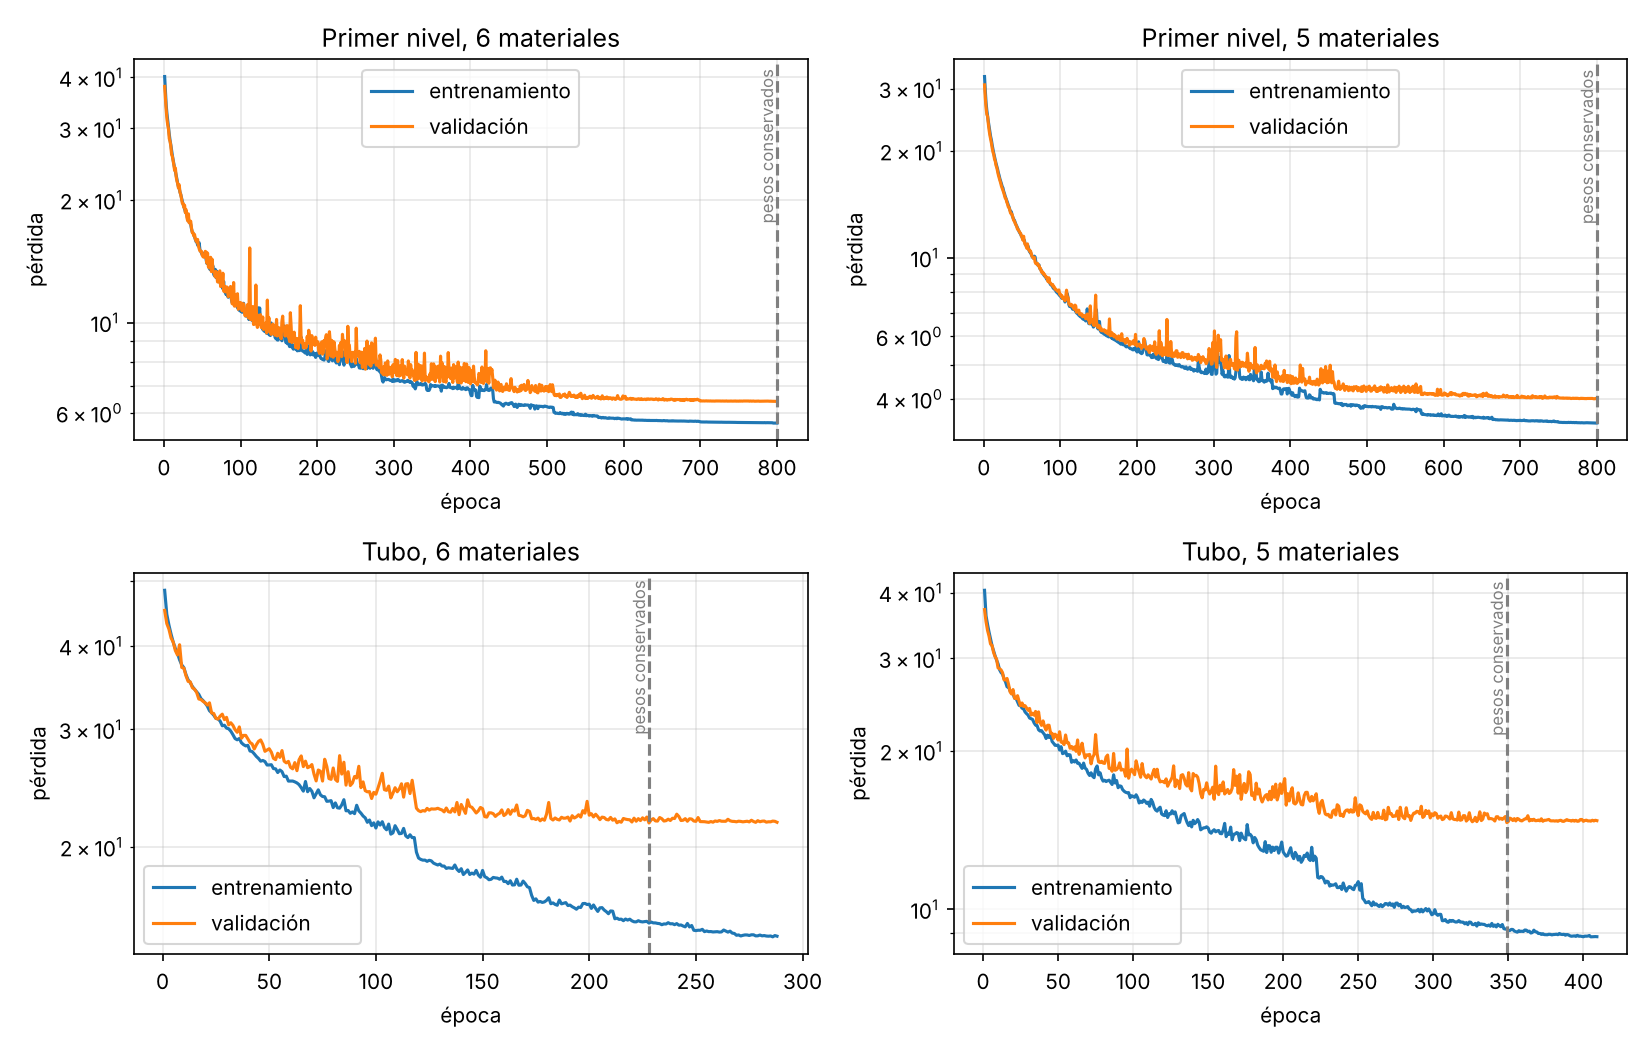
\includegraphics[width=\textwidth]{curvas_aprendizaje_v59_es.png}
\caption{Curvas de aprendizaje: pérdida en entrenamiento (azul) y en validación (naranja) por época, en escala logarítmica. La línea de trazos marca la época cuyos pesos se conservan. La pérdida registrada durante el entrenamiento incluye el término de regularización L2. Arriba, la red en cadena del primer nivel (entropía cruzada binaria sumada sobre las 20 preguntas y los materiales); abajo, la del tubo (la misma suma más 5 veces el error cuadrático medio de $\delta$ estandarizado). En la red del primer nivel se conservan los pesos finales; en la del tubo, los del mínimo de validación.}\label{fig:aprendizaje}
\end{figure}

\begin{table}[H]\centering\small
\caption{Resumen del entrenamiento. Épocas: total corridas y época cuyos pesos se conservan. Pérdida sin el término L2, calculada con los pesos conservados; las dos redes usan la entropía cruzada binaria sumada sobre las preguntas y los materiales (en nats); la del tubo suma además 5 veces el error cuadrático medio de $\delta$ estandarizado, que es menor que 0,02. La última columna es la pérdida de prueba dividida por la de entrenamiento.}\label{tab:entrenamiento}
\resizebox{\textwidth}{!}{\begin{tabular}{llcccccc}\toprule
Red & Datos (entr./val./prueba) & Épocas & Reducc.\ de la tasa & Entr. & Val. & Prueba & Prueba/entr.\\\midrule
Red en cadena, 6 mat. & 24\,151 / 3451 / 6901 & 800 / 800 & 7 & 5,65 & 6,39 & 6,39 & 1,13\\
Red en cadena, 5 mat. & 24\,236 / 3463 / 6925 & 800 / 800 & 5 & 3,40 & 3,98 & 3,99 & 1,17\\
Red en cadena del tubo, 6 mat. & 11\,220 / 1530 / 2250 & 288 / 228 & 5 & 14,91 & 21,72 & 22,57 & 1,51\\
Red en cadena del tubo, 5 mat. & 11\,220 / 1530 / 2250 & 409 / 349 & 6 & 8,88 & 14,61 & 14,69 & 1,65\\\bottomrule
\end{tabular}}
\end{table}

\paragraph{Red en cadena del primer nivel.} Las dos redes llegaron al máximo de 800 épocas; en las últimas la pérdida de validación ya casi no baja, y se conservan los pesos finales. La pérdida de validación queda algo por encima de la de entrenamiento (cociente de 1,13 y 1,17), y la de prueba queda igual a la de validación (6,39 y 3,99 contra 6,39 y 3,98): la red no se degrada con curvas nuevas. Que la pérdida no baje más tiene una razón propia del problema: varias combinaciones enteras reproducen casi igual la misma curva, y la etiqueta (el minimax de la curva con ruido) elige una sola. La red da exactamente las láminas del minimax en el 8,9\,\% de las curvas de prueba con 6 materiales y en el 21,7\,\% con 5, y a lo sumo a una lámina de él en cada material en el 30,2 y el 55,8\,\%; aun así, su diseño cumple la meta en 1998 y 2000 de las 2000 curvas del espacio de trabajo (Tabla~\ref{tab:resumen}). Por eso la red se juzga por el error en la curva, que es el criterio de diseño, y no por coincidir con el minimax.

\paragraph{Red en cadena del tubo.} La validación se separa del entrenamiento desde las primeras 30 épocas y se estabiliza, mientras el entrenamiento sigue bajando. La parada temprana conserva los pesos del mínimo de validación, y la pérdida de prueba queda cerca de la de validación (22,57 contra 21,72 y 14,69 contra 14,61): la red no se degrada con curvas nuevas. La pérdida es más alta que en el primer nivel, y la razón está en el problema y no en la red: en el tubo hay todavía más diseños enteros con casi la misma curva.

\emph{Condicionamiento.} Para 60 arterias de las familias fisiológicas (con los módulos sin recalibrar) se calculó la matriz jacobiana $\mathbf{D}$ de la curva del injerto respecto del diseño $\theta=(h_1\ldots h_N,\delta)$, por diferencias finitas, con cada parámetro en desvíos estándar y la curva en \% de su rango. Con 6 materiales, en la dirección más sensible la curva cambia 8,5 veces su rango por desvío; en la menos sensible, apenas un 1\,\%. El número de condición tiene una mediana de 900 con 6 materiales y 300 con 5, contra $\mathrm{cond}(A)=28$ en el primer nivel. La dirección menos sensible es, típicamente, más espesor de un material y menos de su vecino. Desde la curva, esos diseños son indistinguibles para cualquier método, y la red no puede adivinar cuál de ellos es la etiqueta.

\emph{La medida que importa.} La red da exactamente las láminas del minimax en el 7\,\% de las arterias sintéticas de prueba con 6 materiales y en el 26\,\% con 5; aun así, con la revisión de $\pm1$, su diseño cumple la meta en 294 y 297 de 300. Como en el primer nivel, la red se juzga por el error en la curva y no por coincidir con el minimax.

\clearpage
\section{Láminas y errores de cada curva}\label{sec:tablas}
\textbf{Primer nivel, curva tensión--estiramiento} (Tablas~\ref{tab:suj6} a \ref{tab:ext5}): láminas enteras de cada material y errores de la red en cadena, de la red en cadena con búsqueda de $\pm1$ y del minimax, en los 41 sujetos de Masson y en las 63 curvas externas dentro de $y_1$--$y_2$, con 6 y con 5 materiales. \textbf{Nivel del tubo, curva presión--diámetro} (Tablas~\ref{tab:tubo6} y \ref{tab:tubo5}): láminas de cada capa, preestiramiento y errores de la red en cadena con revisión de $\pm1$ y del minimax de tres pasos, en los 41 sujetos. Las láminas se listan del material 1 al $N$.
{\scriptsize\setlength{\tabcolsep}{2.4pt}
\begin{longtable}{llccccccccc}
\caption{Los 41 sujetos de Masson, 6 materiales: láminas enteras de cada material ($n_1\ldots n_6$) y errores contra la curva del sujeto, $E_{\mathrm{rms}}$ y $e_{\max}$ [\% del rango]. Conj.: E, entrenamiento; P, prueba. En negrita, $e_{\max}>3$\,\%.}\label{tab:suj6}\\\toprule
Sujeto & Conj. & \multicolumn{3}{c}{Red en cadena} & \multicolumn{3}{c}{Red en cadena + $\pm1$} & \multicolumn{3}{c}{Minimax}\\
\cmidrule(lr){3-5}\cmidrule(lr){6-8}\cmidrule(lr){9-11}
 & & láminas & $E_{\mathrm{rms}}$ & $e_{\max}$ & láminas & $E_{\mathrm{rms}}$ & $e_{\max}$ & láminas & $E_{\mathrm{rms}}$ & $e_{\max}$\\\midrule\endfirsthead
\toprule Sujeto & Conj. & \multicolumn{3}{c}{Red en cadena} & \multicolumn{3}{c}{Red en cadena + $\pm1$} & \multicolumn{3}{c}{Minimax}\\\cmidrule(lr){3-5}\cmidrule(lr){6-8}\cmidrule(lr){9-11} & & láminas & $E_{\mathrm{rms}}$ & $e_{\max}$ & láminas & $E_{\mathrm{rms}}$ & $e_{\max}$ & láminas & $E_{\mathrm{rms}}$ & $e_{\max}$\\\midrule\endhead
\bottomrule\endfoot
NT01 & E & 5\enspace 7\enspace 5\enspace 6\enspace 6\enspace 7 & 0,66 & 1,11 & 5\enspace 7\enspace 5\enspace 6\enspace 6\enspace 7 & 0,66 & 1,11 & 5\enspace 7\enspace 5\enspace 6\enspace 7\enspace 5 & 0,72 & 1,11\\
NT02 & P & 9\enspace 3\enspace 2\enspace 5\enspace 3\enspace 4 & 0,54 & 1,55 & 9\enspace 3\enspace 2\enspace 5\enspace 3\enspace 4 & 0,54 & 1,55 & 9\enspace 3\enspace 3\enspace 3\enspace 4\enspace 5 & 0,66 & 1,31\\
NT03 & E & 9\enspace 4\enspace 0\enspace 3\enspace 1\enspace 2 & 1,11 & 1,96 & 9\enspace 4\enspace 0\enspace 3\enspace 1\enspace 2 & 1,11 & 1,96 & 9\enspace 4\enspace 0\enspace 3\enspace 2\enspace 0 & 1,21 & 1,96\\
NT04 & E & 11\enspace 2\enspace 0\enspace 0\enspace 2\enspace 0 & 1,41 & 2,34 & 11\enspace 2\enspace 0\enspace 0\enspace 2\enspace 0 & 1,41 & 2,34 & 11\enspace 2\enspace 0\enspace 0\enspace 2\enspace 0 & 1,41 & 2,34\\
NT05 & E & 11\enspace 5\enspace 5\enspace 2\enspace 4\enspace 3 & 0,62 & 1,53 & 11\enspace 5\enspace 5\enspace 2\enspace 4\enspace 3 & 0,62 & 1,53 & 11\enspace 6\enspace 1\enspace 5\enspace 4\enspace 1 & 0,94 & 1,45\\
NT06 & E & 7\enspace 6\enspace 6\enspace 3\enspace 5\enspace 4 & 0,62 & 1,61 & 7\enspace 6\enspace 6\enspace 4\enspace 4\enspace 4 & 0,48 & 1,51 & 7\enspace 7\enspace 3\enspace 5\enspace 4\enspace 4 & 0,89 & 1,41\\
NT07 & E & 11\enspace 6\enspace 5\enspace 3\enspace 3\enspace 2 & 0,77 & 2,26 & 10\enspace 7\enspace 4\enspace 3\enspace 3\enspace 2 & 1,52 & 2,18 & 10\enspace 8\enspace 2\enspace 3\enspace 4\enspace 1 & 0,55 & 1,34\\
NT08 & P & 5\enspace 3\enspace 2\enspace 1\enspace 2\enspace 1 & 0,81 & 2,82 & 5\enspace 3\enspace 2\enspace 2\enspace 1\enspace 1 & 0,74 & 1,61 & 5\enspace 3\enspace 2\enspace 2\enspace 1\enspace 1 & 0,74 & 1,61\\
NT09 & E & 9\enspace 6\enspace 8\enspace 6\enspace 5\enspace 6 & 0,74 & 1,86 & 9\enspace 6\enspace 8\enspace 6\enspace 5\enspace 6 & 0,74 & 1,86 & 8\enspace 8\enspace 5\enspace 7\enspace 5\enspace 6 & 0,49 & 0,92\\
NT10 & P & 13\enspace 11\enspace 16\enspace 16\enspace 12\enspace 15 & 0,56 & 1,23 & 13\enspace 11\enspace 16\enspace 15\enspace 13\enspace 14 & 0,39 & 1,01 & 13\enspace 12\enspace 13\enspace 15\enspace 15\enspace 12 & 0,56 & 0,97\\
NT11 & P & 11\enspace 14\enspace 16\enspace 17\enspace 15\enspace 16 & 0,68 & 2,02 & 12\enspace 13\enspace 16\enspace 17\enspace 16\enspace 16 & 0,41 & 1,02 & 12\enspace 13\enspace 16\enspace 18\enspace 15\enspace 16 & 0,47 & 1,02\\
NT12 & E & 7\enspace 6\enspace 5\enspace 5\enspace 5\enspace 5 & 0,36 & 1,02 & 7\enspace 6\enspace 6\enspace 4\enspace 5\enspace 5 & 0,47 & 0,96 & 7\enspace 6\enspace 6\enspace 4\enspace 5\enspace 5 & 0,47 & 0,96\\
NT13 & E & 8\enspace 7\enspace 5\enspace 6\enspace 4\enspace 5 & 0,77 & 1,44 & 8\enspace 7\enspace 5\enspace 5\enspace 5\enspace 5 & 0,81 & 1,44 & 8\enspace 7\enspace 5\enspace 5\enspace 7\enspace 1 & 0,87 & 1,44\\
NT14 & E & 7\enspace 6\enspace 3\enspace 4\enspace 4\enspace 3 & 0,62 & 1,47 & 7\enspace 6\enspace 3\enspace 4\enspace 4\enspace 3 & 0,62 & 1,47 & 7\enspace 6\enspace 3\enspace 4\enspace 4\enspace 3 & 0,62 & 1,47\\
NT15 & E & 4\enspace 6\enspace 5\enspace 4\enspace 4\enspace 4 & 0,56 & 1,38 & 4\enspace 6\enspace 5\enspace 4\enspace 4\enspace 4 & 0,56 & 1,38 & 4\enspace 6\enspace 5\enspace 4\enspace 4\enspace 5 & 0,61 & 1,38\\
NT16 & E & 3\enspace 12\enspace 18\enspace 11\enspace 15\enspace 14 & 1,02 & 1,70 & 2\enspace 13\enspace 17\enspace 11\enspace 15\enspace 13 & 0,58 & 1,16 & 2\enspace 13\enspace 15\enspace 14\enspace 14\enspace 13 & 0,38 & 0,89\\
HT01 & E & 5\enspace 9\enspace 5\enspace 7\enspace 7\enspace 6 & 0,46 & 0,79 & 5\enspace 9\enspace 5\enspace 7\enspace 7\enspace 6 & 0,46 & 0,79 & 5\enspace 9\enspace 5\enspace 7\enspace 7\enspace 6 & 0,46 & 0,79\\
HT02 & E & 12\enspace 5\enspace 6\enspace 4\enspace 4\enspace 3 & 0,74 & 1,83 & 12\enspace 5\enspace 6\enspace 4\enspace 4\enspace 3 & 0,74 & 1,83 & 11\enspace 7\enspace 3\enspace 4\enspace 6\enspace 1 & 0,60 & 1,40\\
HT03 & P & 4\enspace 9\enspace 7\enspace 6\enspace 7\enspace 6 & 0,36 & 0,95 & 4\enspace 9\enspace 7\enspace 6\enspace 7\enspace 7 & 0,39 & 0,84 & 4\enspace 9\enspace 7\enspace 6\enspace 7\enspace 7 & 0,39 & 0,84\\
HT04 & E & 8\enspace 3\enspace 1\enspace 2\enspace 1\enspace 2 & 0,86 & 2,16 & 8\enspace 3\enspace 2\enspace 1\enspace 1\enspace 2 & 0,75 & 1,59 & 8\enspace 3\enspace 2\enspace 1\enspace 1\enspace 2 & 0,75 & 1,59\\
HT05 & P & 13\enspace 12\enspace 10\enspace 11\enspace 9\enspace 11 & 0,60 & 1,99 & 13\enspace 12\enspace 10\enspace 12\enspace 9\enspace 10 & 0,38 & 1,07 & 13\enspace 12\enspace 10\enspace 11\enspace 12\enspace 7 & 0,42 & 1,09\\
HT06 & E & 12\enspace 14\enspace 14\enspace 17\enspace 15\enspace 14 & 0,64 & 1,29 & 12\enspace 14\enspace 14\enspace 16\enspace 15\enspace 14 & 0,48 & 1,03 & 13\enspace 12\enspace 18\enspace 14\enspace 16\enspace 14 & 0,49 & 0,78\\
HT07 & E & 14\enspace 9\enspace 14\enspace 9\enspace 9\enspace 9 & 0,74 & 1,86 & 13\enspace 10\enspace 13\enspace 8\enspace 10\enspace 9 & 0,77 & 1,75 & 13\enspace 11\enspace 11\enspace 9\enspace 10\enspace 8 & 0,43 & 0,70\\
HT08 & E & 10\enspace 12\enspace 14\enspace 14\enspace 13\enspace 14 & 0,75 & 1,16 & 9\enspace 13\enspace 13\enspace 14\enspace 14\enspace 13 & 0,42 & 1,04 & 10\enspace 11\enspace 17\enspace 12\enspace 16\enspace 10 & 0,51 & 1,00\\
HT09 & E & 19\enspace 11\enspace 15\enspace 8\enspace 14\enspace 8 & 0,73 & 1,58 & 20\enspace 10\enspace 15\enspace 9\enspace 13\enspace 9 & 0,50 & 0,91 & 20\enspace 10\enspace 14\enspace 10\enspace 12\enspace 12 & 0,38 & 0,91\\
HT10 & E & 2\enspace 10\enspace 4\enspace 8\enspace 5\enspace 7 & 0,49 & 1,19 & 2\enspace 10\enspace 5\enspace 7\enspace 5\enspace 7 & 0,65 & 1,13 & 2\enspace 10\enspace 5\enspace 6\enspace 7\enspace 5 & 0,54 & 0,97\\
HT11 & E & 7\enspace 5\enspace 0\enspace 4\enspace 2\enspace 3 & 0,87 & 2,30 & 7\enspace 5\enspace 0\enspace 4\enspace 2\enspace 3 & 0,87 & 2,30 & 7\enspace 5\enspace 1\enspace 2\enspace 3\enspace 3 & 1,11 & 2,30\\
HT12 & E & 8\enspace 6\enspace 5\enspace 3\enspace 4\enspace 3 & 0,39 & 1,13 & 8\enspace 6\enspace 5\enspace 4\enspace 3\enspace 3 & 0,55 & 1,09 & 8\enspace 6\enspace 5\enspace 4\enspace 3\enspace 3 & 0,55 & 1,09\\
HT13 & P & 16\enspace 4\enspace 7\enspace 4\enspace 6\enspace 5 & 0,51 & 1,59 & 16\enspace 4\enspace 7\enspace 4\enspace 7\enspace 4 & 0,45 & 1,22 & 16\enspace 4\enspace 7\enspace 4\enspace 7\enspace 4 & 0,45 & 1,22\\
HT14 & P & 8\enspace 6\enspace 5\enspace 5\enspace 4\enspace 5 & 0,43 & 0,95 & 8\enspace 6\enspace 5\enspace 5\enspace 4\enspace 5 & 0,43 & 0,95 & 8\enspace 6\enspace 5\enspace 5\enspace 4\enspace 5 & 0,43 & 0,95\\
HT15 & E & 10\enspace 10\enspace 8\enspace 9\enspace 7\enspace 7 & 0,39 & 0,79 & 10\enspace 10\enspace 8\enspace 9\enspace 7\enspace 7 & 0,39 & 0,79 & 10\enspace 10\enspace 8\enspace 9\enspace 7\enspace 7 & 0,39 & 0,79\\
HT16 & E & 6\enspace 15\enspace 15\enspace 14\enspace 15\enspace 14 & 0,34 & 0,95 & 6\enspace 15\enspace 15\enspace 14\enspace 15\enspace 14 & 0,34 & 0,95 & 6\enspace 16\enspace 12\enspace 15\enspace 15\enspace 14 & 0,47 & 0,82\\
HT17 & E & 12\enspace 13\enspace 16\enspace 18\enspace 13\enspace 16 & 0,78 & 1,17 & 11\enspace 14\enspace 16\enspace 17\enspace 13\enspace 15 & 0,48 & 0,98 & 11\enspace 14\enspace 16\enspace 16\enspace 15\enspace 15 & 0,43 & 0,79\\
HT18 & E & 10\enspace 5\enspace 5\enspace 4\enspace 5\enspace 3 & 0,38 & 1,26 & 10\enspace 5\enspace 5\enspace 4\enspace 5\enspace 4 & 0,42 & 1,05 & 10\enspace 5\enspace 5\enspace 4\enspace 5\enspace 4 & 0,42 & 1,05\\
HT19 & P & 9\enspace 6\enspace 5\enspace 5\enspace 3\enspace 5 & 0,41 & 1,42 & 9\enspace 6\enspace 5\enspace 5\enspace 4\enspace 4 & 0,42 & 0,97 & 9\enspace 6\enspace 6\enspace 3\enspace 5\enspace 4 & 0,39 & 0,94\\
HT20 & E & 3\enspace 10\enspace 8\enspace 7\enspace 7\enspace 7 & 0,48 & 1,55 & 3\enspace 10\enspace 8\enspace 7\enspace 8\enspace 6 & 0,41 & 1,01 & 3\enspace 10\enspace 8\enspace 7\enspace 8\enspace 7 & 0,44 & 1,01\\
HT21 & E & 11\enspace 5\enspace 6\enspace 3\enspace 4\enspace 4 & 0,51 & 1,25 & 11\enspace 5\enspace 6\enspace 3\enspace 4\enspace 4 & 0,51 & 1,25 & 11\enspace 5\enspace 5\enspace 5\enspace 3\enspace 4 & 0,59 & 1,25\\
HT22 & E & 13\enspace 10\enspace 9\enspace 5\enspace 6\enspace 5 & 0,37 & 0,97 & 13\enspace 10\enspace 8\enspace 6\enspace 6\enspace 5 & 0,33 & 0,97 & 13\enspace 10\enspace 9\enspace 5\enspace 6\enspace 5 & 0,37 & 0,97\\
HT23 & E & 8\enspace 7\enspace 8\enspace 10\enspace 9\enspace 10 & 0,90 & 1,50 & 7\enspace 8\enspace 8\enspace 9\enspace 10\enspace 9 & 0,42 & 0,97 & 7\enspace 8\enspace 8\enspace 9\enspace 10\enspace 9 & 0,42 & 0,97\\
HT24 & P & 13\enspace 8\enspace 10\enspace 8\enspace 8\enspace 8 & 0,36 & 1,12 & 13\enspace 8\enspace 10\enspace 8\enspace 8\enspace 7 & 0,35 & 1,12 & 13\enspace 9\enspace 7\enspace 9\enspace 9\enspace 6 & 0,70 & 1,07\\
HT25 & E & 5\enspace 16\enspace 19\enspace 20\enspace 19\enspace 20 & 1,00 & 2,90 & 6\enspace 15\enspace 19\enspace 19\enspace 18\enspace 19 & 0,37 & 0,88 & 6\enspace 15\enspace 19\enspace 19\enspace 19\enspace 17 & 0,40 & 0,82\\
\end{longtable}}

{\scriptsize\setlength{\tabcolsep}{2.4pt}
\begin{longtable}{llccccccccc}
\caption{Los 41 sujetos de Masson, 5 materiales: láminas enteras de cada material ($n_1\ldots n_5$) y errores contra la curva del sujeto, $E_{\mathrm{rms}}$ y $e_{\max}$ [\% del rango]. Conj.: E, entrenamiento; P, prueba. En negrita, $e_{\max}>3$\,\%.}\label{tab:suj5}\\\toprule
Sujeto & Conj. & \multicolumn{3}{c}{Red en cadena} & \multicolumn{3}{c}{Red en cadena + $\pm1$} & \multicolumn{3}{c}{Minimax}\\
\cmidrule(lr){3-5}\cmidrule(lr){6-8}\cmidrule(lr){9-11}
 & & láminas & $E_{\mathrm{rms}}$ & $e_{\max}$ & láminas & $E_{\mathrm{rms}}$ & $e_{\max}$ & láminas & $E_{\mathrm{rms}}$ & $e_{\max}$\\\midrule\endfirsthead
\toprule Sujeto & Conj. & \multicolumn{3}{c}{Red en cadena} & \multicolumn{3}{c}{Red en cadena + $\pm1$} & \multicolumn{3}{c}{Minimax}\\\cmidrule(lr){3-5}\cmidrule(lr){6-8}\cmidrule(lr){9-11} & & láminas & $E_{\mathrm{rms}}$ & $e_{\max}$ & láminas & $E_{\mathrm{rms}}$ & $e_{\max}$ & láminas & $E_{\mathrm{rms}}$ & $e_{\max}$\\\midrule\endhead
\bottomrule\endfoot
NT01 & E & 5\enspace 7\enspace 5\enspace 7\enspace 5 & 0,72 & 1,86 & 5\enspace 7\enspace 5\enspace 7\enspace 6 & 0,77 & 1,49 & 5\enspace 7\enspace 5\enspace 7\enspace 6 & 0,77 & 1,49\\
NT02 & P & 9\enspace 3\enspace 3\enspace 4\enspace 4 & 0,88 & 2,03 & 9\enspace 3\enspace 3\enspace 4\enspace 4 & 0,88 & 2,03 & 9\enspace 3\enspace 3\enspace 4\enspace 4 & 0,88 & 2,03\\
NT03 & E & 9\enspace 4\enspace 0\enspace 3\enspace 1 & 1,57 & 2,56 & 9\enspace 4\enspace 0\enspace 3\enspace 1 & 1,57 & 2,56 & 9\enspace 4\enspace 0\enspace 3\enspace 1 & 1,57 & 2,56\\
NT04 & E & 11\enspace 2\enspace 0\enspace 1\enspace 0 & 2,32 & \textbf{3,50} & 11\enspace 2\enspace 0\enspace 1\enspace 0 & 2,32 & \textbf{3,50} & 11\enspace 2\enspace 0\enspace 1\enspace 0 & 2,32 & \textbf{3,50}\\
NT05 & E & 11\enspace 5\enspace 5\enspace 2\enspace 3 & 0,78 & 1,99 & 11\enspace 5\enspace 4\enspace 3\enspace 4 & 0,86 & 1,99 & 11\enspace 6\enspace 2\enspace 4\enspace 3 & 1,18 & 1,90\\
NT06 & E & 7\enspace 7\enspace 3\enspace 5\enspace 4 & 1,00 & 1,68 & 7\enspace 7\enspace 3\enspace 5\enspace 4 & 1,00 & 1,68 & 7\enspace 7\enspace 3\enspace 5\enspace 4 & 1,00 & 1,68\\
NT07 & E & 11\enspace 6\enspace 5\enspace 2\enspace 3 & 0,81 & 2,31 & 11\enspace 6\enspace 4\enspace 3\enspace 3 & 1,17 & 2,31 & 10\enspace 8\enspace 2\enspace 4\enspace 1 & 0,87 & 1,76\\
NT08 & P & 5\enspace 3\enspace 2\enspace 1\enspace 2 & 0,57 & 1,62 & 5\enspace 3\enspace 2\enspace 1\enspace 2 & 0,57 & 1,62 & 5\enspace 3\enspace 2\enspace 1\enspace 2 & 0,57 & 1,62\\
NT09 & E & 8\enspace 8\enspace 5\enspace 6\enspace 6 & 0,68 & 2,03 & 8\enspace 8\enspace 6\enspace 5\enspace 6 & 0,69 & 1,36 & 8\enspace 8\enspace 6\enspace 5\enspace 6 & 0,69 & 1,36\\
NT10 & P & 12\enspace 13\enspace 14\enspace 14\enspace 14 & 0,63 & 1,62 & 13\enspace 12\enspace 15\enspace 14\enspace 14 & 0,72 & 1,13 & 13\enspace 12\enspace 15\enspace 14\enspace 14 & 0,72 & 1,13\\
NT11 & P & 12\enspace 13\enspace 17\enspace 16\enspace 16 & 0,64 & 1,83 & 13\enspace 12\enspace 18\enspace 16\enspace 16 & 0,69 & 1,21 & 13\enspace 12\enspace 18\enspace 16\enspace 16 & 0,69 & 1,21\\
NT12 & E & 7\enspace 6\enspace 5\enspace 5\enspace 5 & 0,54 & 1,52 & 7\enspace 6\enspace 5\enspace 5\enspace 5 & 0,54 & 1,52 & 7\enspace 6\enspace 5\enspace 5\enspace 5 & 0,54 & 1,52\\
NT13 & E & 7\enspace 8\enspace 5\enspace 5\enspace 4 & 0,69 & 2,01 & 8\enspace 7\enspace 6\enspace 4\enspace 5 & 0,96 & 1,48 & 8\enspace 7\enspace 6\enspace 4\enspace 5 & 0,96 & 1,48\\
NT14 & E & 7\enspace 6\enspace 3\enspace 4\enspace 4 & 0,74 & 1,81 & 7\enspace 6\enspace 3\enspace 4\enspace 4 & 0,74 & 1,81 & 7\enspace 6\enspace 3\enspace 4\enspace 4 & 0,74 & 1,81\\
NT15 & E & 4\enspace 6\enspace 5\enspace 4\enspace 4 & 0,65 & 1,40 & 4\enspace 6\enspace 5\enspace 4\enspace 4 & 0,65 & 1,40 & 4\enspace 6\enspace 5\enspace 4\enspace 4 & 0,65 & 1,40\\
NT16 & E & 2\enspace 13\enspace 16\enspace 13\enspace 14 & 0,64 & 1,93 & 3\enspace 12\enspace 16\enspace 14\enspace 13 & 0,72 & 1,67 & 2\enspace 14\enspace 13\enspace 16\enspace 12 & 0,75 & 1,40\\
HT01 & E & 6\enspace 7\enspace 9\enspace 5\enspace 7 & 0,97 & 2,26 & 6\enspace 7\enspace 8\enspace 6\enspace 7 & 0,98 & 2,26 & 5\enspace 9\enspace 6\enspace 6\enspace 8 & 0,73 & 1,42\\
HT02 & E & 11\enspace 7\enspace 3\enspace 5\enspace 3 & 0,69 & 1,70 & 11\enspace 7\enspace 3\enspace 5\enspace 3 & 0,69 & 1,70 & 11\enspace 7\enspace 3\enspace 5\enspace 3 & 0,69 & 1,70\\
HT03 & P & 4\enspace 9\enspace 7\enspace 6\enspace 7 & 0,52 & 1,31 & 4\enspace 9\enspace 7\enspace 6\enspace 7 & 0,52 & 1,31 & 4\enspace 9\enspace 7\enspace 6\enspace 7 & 0,52 & 1,31\\
HT04 & E & 8\enspace 3\enspace 1\enspace 2\enspace 1 & 0,73 & 2,00 & 8\enspace 3\enspace 1\enspace 2\enspace 1 & 0,73 & 2,00 & 8\enspace 3\enspace 1\enspace 2\enspace 1 & 0,73 & 2,00\\
HT05 & P & 14\enspace 11\enspace 11\enspace 11\enspace 10 & 0,70 & 1,27 & 14\enspace 11\enspace 12\enspace 10\enspace 9 & 0,79 & 1,24 & 14\enspace 11\enspace 12\enspace 10\enspace 9 & 0,79 & 1,24\\
HT06 & E & 12\enspace 14\enspace 15\enspace 16\enspace 14 & 0,59 & 1,26 & 12\enspace 14\enspace 15\enspace 16\enspace 14 & 0,59 & 1,26 & 12\enspace 14\enspace 15\enspace 16\enspace 14 & 0,59 & 1,26\\
HT07 & E & 12\enspace 13\enspace 8\enspace 10\enspace 9 & 0,74 & 1,77 & 13\enspace 12\enspace 8\enspace 11\enspace 8 & 0,92 & 1,60 & 13\enspace 11\enspace 11\enspace 9\enspace 10 & 0,58 & 1,22\\
HT08 & E & 9\enspace 13\enspace 14\enspace 13\enspace 14 & 0,60 & 1,76 & 10\enspace 12\enspace 15\enspace 13\enspace 13 & 0,77 & 1,22 & 10\enspace 12\enspace 15\enspace 13\enspace 13 & 0,77 & 1,22\\
HT09 & E & 20\enspace 11\enspace 11\enspace 12\enspace 10 & 0,67 & 1,59 & 20\enspace 11\enspace 11\enspace 12\enspace 11 & 0,66 & 1,19 & 20\enspace 11\enspace 11\enspace 13\enspace 9 & 0,71 & 1,19\\
HT10 & E & 3\enspace 8\enspace 8\enspace 5\enspace 7 & 0,87 & 2,33 & 3\enspace 8\enspace 8\enspace 5\enspace 7 & 0,87 & 2,33 & 2\enspace 10\enspace 5\enspace 7\enspace 6 & 0,73 & 1,44\\
HT11 & E & 8\enspace 3\enspace 4\enspace 2\enspace 3 & 1,15 & 2,50 & 8\enspace 3\enspace 4\enspace 2\enspace 2 & 1,09 & 2,50 & 8\enspace 3\enspace 4\enspace 2\enspace 2 & 1,09 & 2,50\\
HT12 & E & 8\enspace 6\enspace 5\enspace 3\enspace 3 & 0,56 & 1,48 & 8\enspace 6\enspace 5\enspace 3\enspace 3 & 0,56 & 1,48 & 8\enspace 6\enspace 5\enspace 3\enspace 3 & 0,56 & 1,48\\
HT13 & P & 16\enspace 4\enspace 6\enspace 6\enspace 4 & 0,73 & 2,35 & 16\enspace 4\enspace 6\enspace 6\enspace 5 & 0,70 & 1,92 & 16\enspace 5\enspace 4\enspace 7\enspace 4 & 1,11 & 1,65\\
HT14 & P & 8\enspace 6\enspace 5\enspace 5\enspace 4 & 0,54 & 1,02 & 8\enspace 6\enspace 5\enspace 5\enspace 4 & 0,54 & 1,02 & 8\enspace 6\enspace 5\enspace 5\enspace 4 & 0,54 & 1,02\\
HT15 & E & 10\enspace 10\enspace 9\enspace 7\enspace 8 & 0,57 & 1,04 & 10\enspace 10\enspace 9\enspace 7\enspace 8 & 0,57 & 1,04 & 10\enspace 10\enspace 9\enspace 7\enspace 8 & 0,57 & 1,04\\
HT16 & E & 6\enspace 16\enspace 14\enspace 14\enspace 15 & 0,68 & 1,27 & 6\enspace 16\enspace 14\enspace 14\enspace 15 & 0,68 & 1,27 & 6\enspace 16\enspace 13\enspace 16\enspace 13 & 0,61 & 1,27\\
HT17 & E & 11\enspace 15\enspace 15\enspace 16\enspace 15 & 0,88 & 1,43 & 11\enspace 15\enspace 14\enspace 17\enspace 14 & 0,74 & 1,38 & 12\enspace 13\enspace 17\enspace 16\enspace 14 & 0,71 & 1,19\\
HT18 & E & 10\enspace 5\enspace 5\enspace 4\enspace 4 & 0,54 & 1,67 & 10\enspace 5\enspace 5\enspace 4\enspace 5 & 0,57 & 1,59 & 10\enspace 5\enspace 5\enspace 4\enspace 5 & 0,57 & 1,59\\
HT19 & P & 9\enspace 6\enspace 5\enspace 4\enspace 4 & 0,62 & 1,99 & 9\enspace 6\enspace 5\enspace 5\enspace 3 & 0,62 & 1,51 & 9\enspace 6\enspace 6\enspace 3\enspace 5 & 0,79 & 1,51\\
HT20 & E & 2\enspace 12\enspace 5\enspace 8\enspace 7 & 0,79 & 2,05 & 3\enspace 11\enspace 6\enspace 8\enspace 6 & 1,01 & 1,58 & 3\enspace 11\enspace 6\enspace 8\enspace 6 & 1,01 & 1,58\\
HT21 & E & 11\enspace 5\enspace 5\enspace 4\enspace 3 & 0,72 & 1,90 & 11\enspace 5\enspace 5\enspace 4\enspace 4 & 0,71 & 1,82 & 11\enspace 5\enspace 6\enspace 3\enspace 4 & 0,96 & 1,82\\
HT22 & E & 13\enspace 10\enspace 8\enspace 5\enspace 6 & 0,47 & 1,55 & 13\enspace 10\enspace 8\enspace 5\enspace 5 & 0,51 & 1,55 & 13\enspace 11\enspace 5\enspace 8\enspace 3 & 0,88 & 1,47\\
HT23 & E & 7\enspace 8\enspace 9\enspace 9\enspace 10 & 0,66 & 1,28 & 7\enspace 8\enspace 9\enspace 9\enspace 10 & 0,66 & 1,28 & 7\enspace 8\enspace 9\enspace 9\enspace 10 & 0,66 & 1,28\\
HT24 & P & 13\enspace 9\enspace 8\enspace 9\enspace 7 & 0,96 & 1,62 & 13\enspace 9\enspace 8\enspace 8\enspace 8 & 0,79 & 1,34 & 13\enspace 9\enspace 8\enspace 8\enspace 8 & 0,79 & 1,34\\
HT25 & E & 5\enspace 17\enspace 18\enspace 19\enspace 18 & 0,68 & 1,55 & 6\enspace 16\enspace 18\enspace 19\enspace 19 & 0,65 & 1,20 & 6\enspace 16\enspace 18\enspace 19\enspace 19 & 0,65 & 1,20\\
\end{longtable}}

{\scriptsize\setlength{\tabcolsep}{2.4pt}
\begin{longtable}{lccccccccc}
\caption{Validación externa, 6 materiales: las 63 curvas de otros autores dentro de $y_1$--$y_2$. Láminas enteras de cada material y errores $E_{\mathrm{rms}}$ y $e_{\max}$ [\% del rango]. En negrita, $e_{\max}>3$\,\%.}\label{tab:ext6}\\\toprule
Estudio · espécimen · curva & \multicolumn{3}{c}{Red en cadena} & \multicolumn{3}{c}{Red en cadena + $\pm1$} & \multicolumn{3}{c}{Minimax}\\
\cmidrule(lr){2-4}\cmidrule(lr){5-7}\cmidrule(lr){8-10}
& láminas & $E_{\mathrm{rms}}$ & $e_{\max}$ & láminas & $E_{\mathrm{rms}}$ & $e_{\max}$ & láminas & $E_{\mathrm{rms}}$ & $e_{\max}$\\\midrule\endfirsthead
\toprule Estudio · espécimen · curva & \multicolumn{3}{c}{Red en cadena} & \multicolumn{3}{c}{Red en cadena + $\pm1$} & \multicolumn{3}{c}{Minimax}\\\cmidrule(lr){2-4}\cmidrule(lr){5-7}\cmidrule(lr){8-10}& láminas & $E_{\mathrm{rms}}$ & $e_{\max}$ & láminas & $E_{\mathrm{rms}}$ & $e_{\max}$ & láminas & $E_{\mathrm{rms}}$ & $e_{\max}$\\\midrule\endhead
\bottomrule\endfoot
Sommer · CCA pared · I l & 10\enspace 6\enspace 3\enspace 2\enspace 1\enspace 0 & 0,51 & 1,07 & 10\enspace 6\enspace 3\enspace 2\enspace 1\enspace 0 & 0,51 & 1,07 & 10\enspace 6\enspace 3\enspace 2\enspace 0\enspace 2 & 0,39 & 0,97\\
Sommer · CCA pared · II l & 11\enspace 5\enspace 8\enspace 2\enspace 3\enspace 1 & 0,74 & 2,12 & 11\enspace 5\enspace 7\enspace 3\enspace 2\enspace 2 & 0,80 & 2,12 & 11\enspace 6\enspace 4\enspace 4\enspace 2\enspace 2 & 0,94 & 1,68\\
Sommer · CCA pared · II r & 13\enspace 4\enspace 8\enspace 5\enspace 5\enspace 4 & 1,00 & 1,47 & 13\enspace 4\enspace 7\enspace 6\enspace 4\enspace 4 & 0,77 & 1,39 & 13\enspace 4\enspace 7\enspace 7\enspace 3\enspace 5 & 0,83 & 1,39\\
Sommer · CCA pared · IV l & 11\enspace 3\enspace 5\enspace 3\enspace 3\enspace 0 & 1,64 & 2,45 & 11\enspace 3\enspace 4\enspace 3\enspace 3\enspace 1 & 1,58 & 2,45 & 11\enspace 3\enspace 5\enspace 3\enspace 2\enspace 1 & 1,50 & 2,45\\
Sommer · CCA pared · V l & 11\enspace 5\enspace 5\enspace 2\enspace 3\enspace 1 & 0,81 & 1,96 & 11\enspace 5\enspace 4\enspace 3\enspace 2\enspace 1 & 0,80 & 1,96 & 11\enspace 5\enspace 4\enspace 3\enspace 3\enspace 0 & 0,67 & 1,96\\
Sommer · CCA pared · V r & 13\enspace 5\enspace 8\enspace 5\enspace 4\enspace 1 & 0,71 & 2,60 & 14\enspace 4\enspace 7\enspace 6\enspace 5\enspace 1 & 1,00 & 1,73 & 14\enspace 4\enspace 9\enspace 3\enspace 7\enspace 1 & 1,07 & 1,73\\
Sommer · CCA pared · VI l & 10\enspace 3\enspace 7\enspace 2\enspace 3\enspace 2 & 0,77 & 1,98 & 10\enspace 3\enspace 6\enspace 3\enspace 3\enspace 2 & 0,59 & 1,98 & 10\enspace 4\enspace 3\enspace 4\enspace 4\enspace 0 & 1,21 & 1,93\\
Sommer · CCA pared · VI r & 12\enspace 4\enspace 7\enspace 5\enspace 8\enspace 5 & 0,75 & 1,46 & 12\enspace 4\enspace 7\enspace 5\enspace 7\enspace 6 & 0,73 & 1,46 & 12\enspace 4\enspace 6\enspace 7\enspace 6\enspace 6 & 0,50 & 1,04\\
Sommer · CCA pared · VII r & 11\enspace 2\enspace 5\enspace 5\enspace 5\enspace 4 & 2,53 & \textbf{3,62} & 11\enspace 1\enspace 6\enspace 6\enspace 4\enspace 4 & 0,67 & 1,41 & 11\enspace 1\enspace 7\enspace 4\enspace 5\enspace 4 & 0,60 & 1,32\\
Sommer · CCA pared · VIII r & 10\enspace 4\enspace 4\enspace 4\enspace 3\enspace 1 & 0,94 & 2,91 & 11\enspace 3\enspace 3\enspace 5\enspace 4\enspace 1 & 1,70 & 2,64 & 11\enspace 2\enspace 8\enspace 2\enspace 5\enspace 0 & 0,95 & 1,84\\
Sommer · CCA pared · IX r & 11\enspace 4\enspace 5\enspace 3\enspace 2\enspace 1 & 1,00 & 1,74 & 11\enspace 4\enspace 5\enspace 2\enspace 3\enspace 0 & 0,97 & 1,74 & 11\enspace 4\enspace 5\enspace 2\enspace 3\enspace 0 & 0,97 & 1,74\\
Sommer · CCA media-íntima · II l & 17\enspace 9\enspace 6\enspace 7\enspace 7\enspace 6 & 0,55 & 0,92 & 17\enspace 9\enspace 6\enspace 7\enspace 7\enspace 6 & 0,55 & 0,92 & 17\enspace 9\enspace 6\enspace 7\enspace 6\enspace 8 & 0,51 & 0,86\\
Sommer · CCA media-íntima · IV l & 17\enspace 6\enspace 9\enspace 7\enspace 4\enspace 5 & 0,55 & 1,52 & 17\enspace 6\enspace 9\enspace 6\enspace 5\enspace 4 & 0,73 & 1,52 & 17\enspace 7\enspace 7\enspace 6\enspace 7\enspace 1 & 0,79 & 1,29\\
Sommer · CCA media-íntima · V r & 17\enspace 8\enspace 6\enspace 7\enspace 4\enspace 5 & 0,69 & 1,37 & 17\enspace 8\enspace 6\enspace 7\enspace 5\enspace 4 & 0,61 & 1,12 & 17\enspace 8\enspace 7\enspace 6\enspace 5\enspace 4 & 0,66 & 1,12\\
Sommer · CCA media-íntima · VI r & 17\enspace 15\enspace 3\enspace 5\enspace 1\enspace 4 & 0,65 & 1,31 & 17\enspace 15\enspace 4\enspace 5\enspace 0\enspace 3 & 0,54 & 0,98 & 17\enspace 15\enspace 4\enspace 4\enspace 3\enspace 0 & 0,52 & 0,98\\
Sommer · ICA pared · III l & 8\enspace 5\enspace 1\enspace 3\enspace 1\enspace 1 & 1,37 & 2,19 & 8\enspace 5\enspace 0\enspace 4\enspace 1\enspace 0 & 1,29 & 2,19 & 8\enspace 4\enspace 4\enspace 1\enspace 3\enspace 0 & 1,05 & 2,00\\
Sommer · ICA pared · IV l & 11\enspace 5\enspace 4\enspace 6\enspace 3\enspace 1 & 0,89 & 2,19 & 11\enspace 5\enspace 4\enspace 6\enspace 3\enspace 2 & 0,84 & 1,51 & 11\enspace 5\enspace 4\enspace 7\enspace 1\enspace 3 & 0,95 & 1,51\\
Sommer · ICA pared · V r & 10\enspace 4\enspace 6\enspace 2\enspace 4\enspace 1 & 0,77 & 1,63 & 10\enspace 4\enspace 6\enspace 2\enspace 4\enspace 1 & 0,77 & 1,63 & 10\enspace 4\enspace 6\enspace 2\enspace 4\enspace 1 & 0,77 & 1,63\\
Sommer · ICA pared · VI l & 8\enspace 4\enspace 3\enspace 2\enspace 1\enspace 2 & 1,17 & 2,76 & 8\enspace 4\enspace 3\enspace 2\enspace 2\enspace 1 & 0,86 & 2,48 & 8\enspace 4\enspace 3\enspace 3\enspace 1\enspace 0 & 0,90 & 2,48\\
Sommer · ICA pared · VI r & 12\enspace 5\enspace 4\enspace 4\enspace 1\enspace 2 & 0,65 & 1,20 & 12\enspace 5\enspace 4\enspace 4\enspace 1\enspace 2 & 0,65 & 1,20 & 12\enspace 5\enspace 4\enspace 4\enspace 2\enspace 0 & 0,64 & 1,20\\
Sommer · ICA pared · VII r & 8\enspace 4\enspace 3\enspace 2\enspace 1\enspace 2 & 1,66 & \textbf{3,45} & 8\enspace 4\enspace 3\enspace 2\enspace 2\enspace 1 & 1,30 & 2,52 & 8\enspace 4\enspace 4\enspace 1\enspace 3\enspace 0 & 1,09 & 2,52\\
Sommer · ICA pared · VIII r & 10\enspace 3\enspace 7\enspace 3\enspace 3\enspace 3 & 1,08 & 2,53 & 11\enspace 2\enspace 6\enspace 4\enspace 4\enspace 2 & 1,06 & 2,00 & 11\enspace 2\enspace 7\enspace 3\enspace 5\enspace 0 & 1,34 & 2,00\\
Sommer · ICA pared · IX r & 9\enspace 3\enspace 4\enspace 3\enspace 1\enspace 3 & 1,57 & \textbf{3,17} & 9\enspace 3\enspace 3\enspace 3\enspace 2\enspace 2 & 1,52 & 2,35 & 9\enspace 3\enspace 3\enspace 5\enspace 0\enspace 2 & 1,59 & 2,35\\
Sommer · ICA pared · X r & 10\enspace 2\enspace 7\enspace 2\enspace 2\enspace 2 & 1,27 & 2,43 & 10\enspace 2\enspace 6\enspace 3\enspace 2\enspace 1 & 1,36 & 2,43 & 9\enspace 4\enspace 3\enspace 4\enspace 1\enspace 2 & 0,89 & 1,76\\
Sommer · ICA pared · XI r & 11\enspace 4\enspace 5\enspace 3\enspace 2\enspace 1 & 0,56 & 1,23 & 11\enspace 4\enspace 5\enspace 3\enspace 2\enspace 1 & 0,56 & 1,23 & 11\enspace 4\enspace 5\enspace 3\enspace 2\enspace 1 & 0,56 & 1,23\\
Sommer · ICA media-íntima · IX r & 17\enspace 8\enspace 9\enspace 4\enspace 4\enspace 2 & 0,58 & 1,09 & 17\enspace 8\enspace 8\enspace 5\enspace 4\enspace 2 & 0,52 & 1,09 & 17\enspace 8\enspace 8\enspace 5\enspace 5\enspace 0 & 0,53 & 1,09\\
Sommer · ICA media-íntima · X r & 14\enspace 4\enspace 10\enspace 3\enspace 4\enspace 1 & 1,28 & \textbf{4,22} & 15\enspace 3\enspace 10\enspace 4\enspace 4\enspace 2 & 1,04 & 1,91 & 14\enspace 5\enspace 7\enspace 5\enspace 4\enspace 2 & 0,59 & 1,04\\
Sommer · ICA media-íntima · XI r & 14\enspace 5\enspace 8\enspace 3\enspace 4\enspace 0 & 0,76 & 1,90 & 14\enspace 5\enspace 8\enspace 4\enspace 3\enspace 0 & 0,61 & 1,52 & 14\enspace 5\enspace 9\enspace 3\enspace 3\enspace 0 & 0,72 & 1,52\\
Liu · carótida con placa · P2 & 13\enspace 2\enspace 3\enspace 1\enspace 0\enspace 1 & 1,02 & 2,57 & 13\enspace 2\enspace 3\enspace 0\enspace 1\enspace 1 & 1,37 & 2,57 & 13\enspace 2\enspace 4\enspace 0\enspace 0\enspace 1 & 1,45 & 2,57\\
Liu · carótida con placa · P4 & 18\enspace 2\enspace 0\enspace 1\enspace 0\enspace 0 & 1,03 & 1,65 & 18\enspace 2\enspace 0\enspace 1\enspace 0\enspace 0 & 1,03 & 1,65 & 18\enspace 2\enspace 0\enspace 1\enspace 0\enspace 0 & 1,03 & 1,65\\
Liu · carótida con placa · P5 & 11\enspace 1\enspace 0\enspace 0\enspace 0\enspace 1 & 2,72 & \textbf{4,41} & 11\enspace 1\enspace 0\enspace 0\enspace 1\enspace 0 & 2,37 & \textbf{3,74} & 11\enspace 1\enspace 0\enspace 0\enspace 1\enspace 0 & 2,37 & \textbf{3,74}\\
Liu · carótida con placa · P6 & 14\enspace 1\enspace 0\enspace 1\enspace 0\enspace 0 & 3,65 & \textbf{4,73} & 13\enspace 2\enspace 0\enspace 0\enspace 0\enspace 0 & 1,66 & \textbf{3,53} & 13\enspace 2\enspace 0\enspace 0\enspace 0\enspace 0 & 1,66 & \textbf{3,53}\\
Liu · carótida con placa · P7 & 11\enspace 2\enspace 0\enspace 0\enspace 0\enspace 0 & 3,00 & \textbf{6,24} & 12\enspace 1\enspace 0\enspace 0\enspace 1\enspace 0 & 1,61 & \textbf{3,54} & 12\enspace 1\enspace 0\enspace 0\enspace 1\enspace 0 & 1,61 & \textbf{3,54}\\
Liu · carótida con placa · P8 & 12\enspace 5\enspace 0\enspace 1\enspace 0\enspace 0 & 1,24 & 1,94 & 12\enspace 5\enspace 0\enspace 0\enspace 1\enspace 0 & 1,17 & 1,94 & 12\enspace 5\enspace 0\enspace 0\enspace 1\enspace 0 & 1,17 & 1,94\\
Liu · carótida con placa · P9 & 15\enspace 6\enspace 1\enspace 1\enspace 0\enspace 0 & 0,72 & 1,34 & 15\enspace 6\enspace 1\enspace 0\enspace 1\enspace 0 & 0,60 & 1,34 & 15\enspace 6\enspace 1\enspace 1\enspace 0\enspace 0 & 0,72 & 1,34\\
Liu · carótida con placa · P10 & 16\enspace 5\enspace 0\enspace 1\enspace 0\enspace 0 & 1,01 & 1,97 & 16\enspace 5\enspace 0\enspace 1\enspace 0\enspace 0 & 1,01 & 1,97 & 16\enspace 5\enspace 0\enspace 1\enspace 0\enspace 0 & 1,01 & 1,97\\
Kamenskiy · CCA · pac. 1 & 15\enspace 10\enspace 4\enspace 1\enspace 0\enspace 0 & 1,70 & 2,87 & 15\enspace 11\enspace 3\enspace 0\enspace 1\enspace 0 & 0,37 & 0,97 & 15\enspace 11\enspace 2\enspace 1\enspace 1\enspace 0 & 0,39 & 0,97\\
Kamenskiy · ECA · pac. 1 & 9\enspace 2\enspace 6\enspace 2\enspace 2\enspace 1 & 1,16 & 1,71 & 9\enspace 2\enspace 5\enspace 3\enspace 2\enspace 1 & 0,77 & 1,55 & 9\enspace 2\enspace 6\enspace 1\enspace 3\enspace 1 & 0,99 & 1,55\\
Kamenskiy · ICA · pac. 1 & 14\enspace 6\enspace 4\enspace 2\enspace 1\enspace 1 & 0,81 & 1,05 & 14\enspace 6\enspace 3\enspace 3\enspace 1\enspace 0 & 0,53 & 1,04 & 14\enspace 6\enspace 4\enspace 1\enspace 2\enspace 1 & 0,66 & 1,04\\
Kamenskiy · CCA · pac. 4 & 9\enspace 5\enspace 0\enspace 2\enspace 0\enspace 0 & 0,79 & 2,33 & 9\enspace 5\enspace 0\enspace 1\enspace 1\enspace 0 & 1,21 & 2,33 & 9\enspace 5\enspace 1\enspace 0\enspace 1\enspace 0 & 0,94 & 2,33\\
Kamenskiy · CCA · pac. 5 & 13\enspace 3\enspace 1\enspace 0\enspace 0\enspace 0 & 1,28 & 2,57 & 13\enspace 3\enspace 1\enspace 0\enspace 0\enspace 0 & 1,28 & 2,57 & 13\enspace 3\enspace 1\enspace 0\enspace 0\enspace 0 & 1,28 & 2,57\\
Kamenskiy · ECA · pac. 5 & 8\enspace 4\enspace 3\enspace 0\enspace 1\enspace 0 & 1,93 & \textbf{3,75} & 8\enspace 4\enspace 3\enspace 0\enspace 0\enspace 1 & 2,16 & \textbf{3,75} & 8\enspace 5\enspace 1\enspace 0\enspace 1\enspace 0 & 0,96 & 1,57\\
Kamenskiy · CCA · pac. 6 & 7\enspace 3\enspace 0\enspace 2\enspace 1\enspace 0 & 2,10 & \textbf{4,79} & 7\enspace 3\enspace 0\enspace 1\enspace 2\enspace 1 & 2,67 & \textbf{4,79} & 8\enspace 1\enspace 3\enspace 2\enspace 1\enspace 0 & 1,38 & 2,57\\
Kamenskiy · ECA · pac. 6 & 8\enspace 3\enspace 0\enspace 2\enspace 0\enspace 1 & 2,06 & \textbf{3,72} & 8\enspace 3\enspace 0\enspace 1\enspace 1\enspace 0 & 2,04 & \textbf{3,72} & 9\enspace 1\enspace 3\enspace 1\enspace 1\enspace 0 & 1,73 & \textbf{3,46}\\
Kamenskiy · ECA · pac. 7 & 12\enspace 1\enspace 3\enspace 0\enspace 1\enspace 0 & 0,89 & 1,74 & 12\enspace 1\enspace 3\enspace 0\enspace 1\enspace 0 & 0,89 & 1,74 & 12\enspace 1\enspace 3\enspace 0\enspace 1\enspace 0 & 0,89 & 1,74\\
Kamenskiy · ICA · pac. 7 & 13\enspace 4\enspace 1\enspace 1\enspace 1\enspace 0 & 0,81 & 2,12 & 13\enspace 4\enspace 1\enspace 1\enspace 1\enspace 0 & 0,81 & 2,12 & 13\enspace 4\enspace 1\enspace 1\enspace 1\enspace 0 & 0,81 & 2,12\\
Kamenskiy · CCA · pac. 8 & 13\enspace 0\enspace 4\enspace 1\enspace 2\enspace 0 & 4,10 & \textbf{7,71} & 13\enspace 1\enspace 3\enspace 1\enspace 2\enspace 0 & 1,22 & 2,12 & 13\enspace 1\enspace 2\enspace 3\enspace 1\enspace 0 & 1,08 & 1,97\\
Kamenskiy · ECA · pac. 8 & 15\enspace 2\enspace 3\enspace 0\enspace 1\enspace 0 & 0,66 & 1,15 & 15\enspace 2\enspace 3\enspace 0\enspace 1\enspace 0 & 0,66 & 1,15 & 15\enspace 2\enspace 3\enspace 0\enspace 1\enspace 0 & 0,66 & 1,15\\
Kamenskiy · ICA · pac. 8 & 14\enspace 2\enspace 4\enspace 1\enspace 2\enspace 0 & 0,94 & 1,80 & 14\enspace 2\enspace 4\enspace 1\enspace 2\enspace 0 & 0,94 & 1,80 & 14\enspace 2\enspace 4\enspace 1\enspace 2\enspace 0 & 0,94 & 1,80\\
Kamenskiy · ECA · pac. 9 & 9\enspace 5\enspace 0\enspace 2\enspace 0\enspace 0 & 1,22 & 2,38 & 9\enspace 5\enspace 0\enspace 1\enspace 1\enspace 0 & 0,87 & 2,38 & 9\enspace 5\enspace 0\enspace 1\enspace 1\enspace 0 & 0,87 & 2,38\\
Kamenskiy · ICA · pac. 9 & 17\enspace 1\enspace 3\enspace 1\enspace 1\enspace 1 & 2,28 & \textbf{4,21} & 17\enspace 1\enspace 4\enspace 1\enspace 0\enspace 2 & 0,98 & 2,13 & 17\enspace 1\enspace 4\enspace 1\enspace 0\enspace 2 & 0,98 & 2,13\\
Kamenskiy · ICA · pac. 10 & 10\enspace 3\enspace 2\enspace 0\enspace 0\enspace 0 & 2,26 & \textbf{4,42} & 10\enspace 3\enspace 2\enspace 0\enspace 0\enspace 0 & 2,26 & \textbf{4,42} & 10\enspace 4\enspace 0\enspace 0\enspace 0\enspace 0 & 1,33 & 1,79\\
Kamenskiy · ICA · pac. 11 & 12\enspace 1\enspace 1\enspace 0\enspace 0\enspace 0 & 4,59 & \textbf{6,16} & 12\enspace 2\enspace 0\enspace 0\enspace 0\enspace 0 & 2,98 & \textbf{5,71} & 12\enspace 2\enspace 0\enspace 0\enspace 0\enspace 0 & 2,98 & \textbf{5,71}\\
Kamenskiy · CCA · pac. 12 & 9\enspace 2\enspace 3\enspace 0\enspace 0\enspace 1 & 1,27 & \textbf{3,21} & 9\enspace 2\enspace 3\enspace 0\enspace 1\enspace 0 & 0,70 & 2,17 & 9\enspace 2\enspace 3\enspace 0\enspace 1\enspace 0 & 0,70 & 2,17\\
Kamenskiy · ECA · pac. 12 & 13\enspace 4\enspace 0\enspace 2\enspace 0\enspace 0 & 1,74 & 2,77 & 13\enspace 4\enspace 0\enspace 1\enspace 1\enspace 1 & 2,06 & 2,77 & 13\enspace 3\enspace 3\enspace 1\enspace 0\enspace 0 & 1,21 & 2,13\\
Kamenskiy · ICA · pac. 12 & 14\enspace 3\enspace 0\enspace 1\enspace 0\enspace 1 & 1,87 & \textbf{3,71} & 14\enspace 3\enspace 1\enspace 0\enspace 1\enspace 0 & 0,87 & 1,34 & 14\enspace 3\enspace 1\enspace 0\enspace 1\enspace 0 & 0,87 & 1,34\\
Kamenskiy · ICA · pac. 13 & 13\enspace 2\enspace 2\enspace 1\enspace 1\enspace 0 & 1,05 & 2,25 & 13\enspace 2\enspace 2\enspace 1\enspace 0\enspace 1 & 0,88 & 2,25 & 13\enspace 2\enspace 2\enspace 1\enspace 1\enspace 0 & 1,05 & 2,25\\
Kamenskiy · CCA · pac. 14 & 12\enspace 1\enspace 3\enspace 0\enspace 1\enspace 0 & 0,75 & 2,17 & 12\enspace 1\enspace 3\enspace 0\enspace 1\enspace 0 & 0,75 & 2,17 & 12\enspace 1\enspace 3\enspace 0\enspace 1\enspace 0 & 0,75 & 2,17\\
Kamenskiy · ICA · pac. 14 & 12\enspace 0\enspace 3\enspace 0\enspace 1\enspace 0 & 2,34 & \textbf{3,23} & 12\enspace 0\enspace 2\enspace 1\enspace 1\enspace 0 & 1,62 & 2,92 & 12\enspace 0\enspace 2\enspace 1\enspace 1\enspace 0 & 1,62 & 2,92\\
Kamenskiy · CCA · pac. 15 & 12\enspace 1\enspace 0\enspace 0\enspace 0\enspace 0 & 4,51 & \textbf{5,53} & 13\enspace 0\enspace 0\enspace 1\enspace 0\enspace 0 & 2,37 & \textbf{4,35} & 13\enspace 0\enspace 0\enspace 1\enspace 0\enspace 0 & 2,37 & \textbf{4,35}\\
Kamenskiy · CCA · pac. 16 & 13\enspace 0\enspace 4\enspace 2\enspace 1\enspace 1 & 2,78 & \textbf{5,53} & 13\enspace 1\enspace 3\enspace 1\enspace 2\enspace 1 & 1,80 & \textbf{3,08} & 13\enspace 1\enspace 2\enspace 2\enspace 2\enspace 1 & 1,43 & 2,28\\
Kamenskiy · ECA · pac. 16 & 10\enspace 2\enspace 3\enspace 1\enspace 1\enspace 0 & 1,01 & 1,91 & 10\enspace 2\enspace 3\enspace 1\enspace 1\enspace 0 & 1,01 & 1,91 & 10\enspace 2\enspace 3\enspace 1\enspace 1\enspace 0 & 1,01 & 1,91\\
Kamenskiy · ICA · pac. 16 & 13\enspace 4\enspace 1\enspace 0\enspace 0\enspace 0 & 1,36 & 2,26 & 13\enspace 4\enspace 1\enspace 0\enspace 0\enspace 0 & 1,36 & 2,26 & 13\enspace 4\enspace 1\enspace 0\enspace 0\enspace 0 & 1,36 & 2,26\\
\end{longtable}}

{\scriptsize\setlength{\tabcolsep}{2.4pt}
\begin{longtable}{lccccccccc}
\caption{Validación externa, 5 materiales: las 63 curvas de otros autores dentro de $y_1$--$y_2$. Láminas enteras de cada material y errores $E_{\mathrm{rms}}$ y $e_{\max}$ [\% del rango]. En negrita, $e_{\max}>3$\,\%.}\label{tab:ext5}\\\toprule
Estudio · espécimen · curva & \multicolumn{3}{c}{Red en cadena} & \multicolumn{3}{c}{Red en cadena + $\pm1$} & \multicolumn{3}{c}{Minimax}\\
\cmidrule(lr){2-4}\cmidrule(lr){5-7}\cmidrule(lr){8-10}
& láminas & $E_{\mathrm{rms}}$ & $e_{\max}$ & láminas & $E_{\mathrm{rms}}$ & $e_{\max}$ & láminas & $E_{\mathrm{rms}}$ & $e_{\max}$\\\midrule\endfirsthead
\toprule Estudio · espécimen · curva & \multicolumn{3}{c}{Red en cadena} & \multicolumn{3}{c}{Red en cadena + $\pm1$} & \multicolumn{3}{c}{Minimax}\\\cmidrule(lr){2-4}\cmidrule(lr){5-7}\cmidrule(lr){8-10}& láminas & $E_{\mathrm{rms}}$ & $e_{\max}$ & láminas & $E_{\mathrm{rms}}$ & $e_{\max}$ & láminas & $E_{\mathrm{rms}}$ & $e_{\max}$\\\midrule\endhead
\bottomrule\endfoot
Sommer · CCA pared · I l & 10\enspace 6\enspace 3\enspace 1\enspace 0 & 0,73 & 1,51 & 10\enspace 6\enspace 3\enspace 1\enspace 0 & 0,73 & 1,51 & 10\enspace 6\enspace 3\enspace 1\enspace 0 & 0,73 & 1,51\\
Sommer · CCA pared · II l & 11\enspace 6\enspace 4\enspace 3\enspace 2 & 1,00 & 1,87 & 11\enspace 6\enspace 4\enspace 3\enspace 2 & 1,00 & 1,87 & 11\enspace 6\enspace 5\enspace 2\enspace 2 & 1,23 & 1,87\\
Sommer · CCA pared · II r & 13\enspace 4\enspace 8\enspace 4\enspace 4 & 0,93 & 1,55 & 13\enspace 4\enspace 8\enspace 4\enspace 4 & 0,93 & 1,55 & 13\enspace 4\enspace 8\enspace 4\enspace 5 & 0,97 & 1,55\\
Sommer · CCA pared · IV l & 11\enspace 3\enspace 5\enspace 2\enspace 2 & 1,55 & 2,63 & 11\enspace 3\enspace 4\enspace 3\enspace 2 & 1,46 & 2,63 & 11\enspace 3\enspace 5\enspace 2\enspace 1 & 1,57 & 2,63\\
Sommer · CCA pared · V l & 11\enspace 5\enspace 4\enspace 3\enspace 0 & 0,76 & 2,11 & 11\enspace 5\enspace 4\enspace 3\enspace 0 & 0,76 & 2,11 & 11\enspace 5\enspace 5\enspace 1\enspace 2 & 1,01 & 2,11\\
Sommer · CCA pared · V r & 13\enspace 5\enspace 8\enspace 3\enspace 4 & 0,93 & 2,27 & 14\enspace 4\enspace 8\enspace 4\enspace 3 & 1,03 & 1,85 & 14\enspace 4\enspace 8\enspace 4\enspace 4 & 0,99 & 1,85\\
Sommer · CCA pared · VI l & 10\enspace 4\enspace 3\enspace 4\enspace 2 & 1,22 & 2,23 & 10\enspace 4\enspace 3\enspace 4\enspace 2 & 1,22 & 2,23 & 10\enspace 4\enspace 3\enspace 4\enspace 2 & 1,22 & 2,23\\
Sommer · CCA pared · VI r & 12\enspace 4\enspace 7\enspace 6\enspace 6 & 0,72 & 1,33 & 12\enspace 4\enspace 7\enspace 6\enspace 6 & 0,72 & 1,33 & 12\enspace 4\enspace 7\enspace 6\enspace 6 & 0,72 & 1,33\\
Sommer · CCA pared · VII r & 11\enspace 2\enspace 4\enspace 6\enspace 4 & 1,57 & 2,67 & 11\enspace 2\enspace 4\enspace 6\enspace 4 & 1,57 & 2,67 & 11\enspace 2\enspace 4\enspace 7\enspace 2 & 1,79 & 2,67\\
Sommer · CCA pared · VIII r & 10\enspace 4\enspace 5\enspace 3\enspace 2 & 1,43 & 2,76 & 10\enspace 4\enspace 4\enspace 4\enspace 2 & 0,91 & 2,76 & 10\enspace 4\enspace 5\enspace 2\enspace 4 & 1,22 & 2,76\\
Sommer · CCA pared · IX r & 11\enspace 4\enspace 5\enspace 2\enspace 1 & 1,13 & 1,87 & 11\enspace 4\enspace 5\enspace 1\enspace 2 & 1,11 & 1,87 & 11\enspace 4\enspace 5\enspace 1\enspace 2 & 1,11 & 1,87\\
Sommer · CCA media-íntima · II l & 17\enspace 8\enspace 8\enspace 6\enspace 7 & 0,74 & 2,07 & 17\enspace 9\enspace 7\enspace 5\enspace 8 & 0,87 & 1,70 & 17\enspace 9\enspace 6\enspace 7\enspace 7 & 0,61 & 1,01\\
Sommer · CCA media-íntima · IV l & 16\enspace 8\enspace 7\enspace 5\enspace 4 & 0,77 & 2,31 & 17\enspace 7\enspace 7\enspace 6\enspace 4 & 0,80 & 1,49 & 17\enspace 7\enspace 7\enspace 6\enspace 4 & 0,80 & 1,49\\
Sommer · CCA media-íntima · V r & 17\enspace 8\enspace 7\enspace 5\enspace 5 & 0,73 & 1,26 & 17\enspace 8\enspace 7\enspace 5\enspace 5 & 0,73 & 1,26 & 17\enspace 8\enspace 7\enspace 5\enspace 5 & 0,73 & 1,26\\
Sommer · CCA media-íntima · VI r & 17\enspace 14\enspace 5\enspace 2\enspace 2 & 0,94 & 1,92 & 17\enspace 15\enspace 4\enspace 2\enspace 2 & 0,79 & 1,20 & 17\enspace 15\enspace 3\enspace 3\enspace 2 & 0,72 & 1,20\\
Sommer · ICA pared · III l & 8\enspace 5\enspace 1\enspace 3\enspace 0 & 1,79 & 2,79 & 8\enspace 5\enspace 1\enspace 2\enspace 1 & 1,78 & 2,79 & 8\enspace 4\enspace 4\enspace 1\enspace 0 & 1,30 & 2,54\\
Sommer · ICA pared · IV l & 11\enspace 5\enspace 5\enspace 4\enspace 3 & 1,00 & 1,79 & 11\enspace 5\enspace 5\enspace 4\enspace 3 & 1,00 & 1,79 & 11\enspace 5\enspace 5\enspace 4\enspace 3 & 1,00 & 1,79\\
Sommer · ICA pared · V r & 10\enspace 4\enspace 6\enspace 2\enspace 2 & 1,27 & 2,30 & 10\enspace 4\enspace 5\enspace 3\enspace 2 & 0,64 & 1,73 & 10\enspace 4\enspace 5\enspace 3\enspace 2 & 0,64 & 1,73\\
Sommer · ICA pared · VI l & 8\enspace 4\enspace 3\enspace 2\enspace 0 & 0,91 & 2,69 & 8\enspace 4\enspace 3\enspace 2\enspace 0 & 0,91 & 2,69 & 8\enspace 4\enspace 4\enspace 0\enspace 2 & 1,35 & 2,69\\
Sommer · ICA pared · VI r & 12\enspace 5\enspace 4\enspace 3\enspace 1 & 0,74 & 1,44 & 12\enspace 5\enspace 4\enspace 3\enspace 1 & 0,74 & 1,44 & 12\enspace 5\enspace 4\enspace 3\enspace 1 & 0,74 & 1,44\\
Sommer · ICA pared · VII r & 8\enspace 5\enspace 1\enspace 3\enspace 0 & 2,22 & \textbf{3,31} & 8\enspace 5\enspace 1\enspace 2\enspace 1 & 2,06 & \textbf{3,31} & 9\enspace 3\enspace 3\enspace 3\enspace 0 & 1,68 & 2,69\\
Sommer · ICA pared · VIII r & 10\enspace 4\enspace 4\enspace 4\enspace 3 & 1,77 & 2,53 & 10\enspace 4\enspace 3\enspace 5\enspace 2 & 1,48 & 2,53 & 11\enspace 2\enspace 7\enspace 2\enspace 4 & 1,33 & 2,14\\
Sommer · ICA pared · IX r & 9\enspace 3\enspace 4\enspace 2\enspace 1 & 1,48 & 2,51 & 9\enspace 3\enspace 4\enspace 2\enspace 1 & 1,48 & 2,51 & 9\enspace 3\enspace 4\enspace 2\enspace 1 & 1,48 & 2,51\\
Sommer · ICA pared · X r & 9\enspace 4\enspace 4\enspace 2\enspace 2 & 1,32 & 2,05 & 9\enspace 4\enspace 3\enspace 3\enspace 2 & 1,02 & 1,86 & 9\enspace 4\enspace 3\enspace 4\enspace 0 & 1,12 & 1,86\\
Sommer · ICA pared · XI r & 11\enspace 4\enspace 5\enspace 2\enspace 1 & 0,76 & 1,44 & 11\enspace 4\enspace 5\enspace 2\enspace 1 & 0,76 & 1,44 & 11\enspace 4\enspace 5\enspace 2\enspace 1 & 0,76 & 1,44\\
Sommer · ICA media-íntima · IX r & 17\enspace 8\enspace 8\enspace 3\enspace 3 & 0,78 & 1,60 & 17\enspace 8\enspace 8\enspace 4\enspace 2 & 0,64 & 1,25 & 17\enspace 8\enspace 8\enspace 4\enspace 3 & 0,71 & 1,25\\
Sommer · ICA media-íntima · X r & 14\enspace 5\enspace 7\enspace 4\enspace 3 & 0,70 & 1,31 & 14\enspace 5\enspace 7\enspace 4\enspace 3 & 0,70 & 1,31 & 14\enspace 5\enspace 7\enspace 4\enspace 3 & 0,70 & 1,31\\
Sommer · ICA media-íntima · XI r & 14\enspace 5\enspace 7\enspace 3\enspace 2 & 1,19 & 2,87 & 14\enspace 6\enspace 6\enspace 2\enspace 3 & 1,35 & 2,30 & 14\enspace 6\enspace 5\enspace 4\enspace 2 & 1,20 & 2,30\\
Liu · carótida con placa · P2 & 12\enspace 3\enspace 2\enspace 0\enspace 1 & 2,11 & \textbf{3,35} & 13\enspace 2\enspace 2\enspace 1\enspace 0 & 1,51 & 2,68 & 13\enspace 2\enspace 2\enspace 1\enspace 0 & 1,51 & 2,68\\
Liu · carótida con placa · P4 & 18\enspace 2\enspace 0\enspace 0\enspace 1 & 1,65 & 2,45 & 18\enspace 2\enspace 0\enspace 0\enspace 1 & 1,65 & 2,45 & 18\enspace 2\enspace 0\enspace 0\enspace 1 & 1,65 & 2,45\\
Liu · carótida con placa · P5 & 11\enspace 1\enspace 0\enspace 0\enspace 1 & 2,83 & \textbf{3,91} & 11\enspace 1\enspace 0\enspace 0\enspace 1 & 2,83 & \textbf{3,91} & 11\enspace 1\enspace 0\enspace 0\enspace 1 & 2,83 & \textbf{3,91}\\
Liu · carótida con placa · P6 & 13\enspace 2\enspace 0\enspace 0\enspace 0 & 2,68 & \textbf{3,75} & 13\enspace 2\enspace 0\enspace 0\enspace 0 & 2,68 & \textbf{3,75} & 13\enspace 2\enspace 0\enspace 0\enspace 0 & 2,68 & \textbf{3,75}\\
Liu · carótida con placa · P7 & 12\enspace 1\enspace 0\enspace 0\enspace 0 & 1,67 & \textbf{3,16} & 12\enspace 1\enspace 0\enspace 0\enspace 0 & 1,67 & \textbf{3,16} & 12\enspace 1\enspace 0\enspace 0\enspace 0 & 1,67 & \textbf{3,16}\\
Liu · carótida con placa · P8 & 12\enspace 4\enspace 2\enspace 0\enspace 0 & 1,28 & 2,84 & 12\enspace 4\enspace 2\enspace 0\enspace 0 & 1,28 & 2,84 & 12\enspace 5\enspace 0\enspace 0\enspace 1 & 1,78 & 2,45\\
Liu · carótida con placa · P9 & 15\enspace 6\enspace 0\enspace 1\enspace 0 & 0,80 & 1,44 & 15\enspace 6\enspace 0\enspace 1\enspace 0 & 0,80 & 1,44 & 15\enspace 6\enspace 0\enspace 1\enspace 0 & 0,80 & 1,44\\
Liu · carótida con placa · P10 & 16\enspace 5\enspace 0\enspace 0\enspace 1 & 1,51 & 2,17 & 16\enspace 5\enspace 0\enspace 0\enspace 1 & 1,51 & 2,17 & 16\enspace 5\enspace 0\enspace 0\enspace 1 & 1,51 & 2,17\\
Kamenskiy · CCA · pac. 1 & 15\enspace 11\enspace 1\enspace 1\enspace 1 & 0,51 & 1,52 & 15\enspace 11\enspace 1\enspace 1\enspace 0 & 0,60 & 1,52 & 15\enspace 11\enspace 1\enspace 1\enspace 1 & 0,51 & 1,52\\
Kamenskiy · ECA · pac. 1 & 9\enspace 3\enspace 3\enspace 3\enspace 1 & 2,78 & \textbf{4,22} & 9\enspace 2\enspace 4\enspace 3\enspace 1 & 1,87 & \textbf{3,98} & 9\enspace 2\enspace 6\enspace 0\enspace 3 & 1,42 & 2,63\\
Kamenskiy · ICA · pac. 1 & 14\enspace 6\enspace 3\enspace 2\enspace 0 & 0,72 & 1,33 & 14\enspace 6\enspace 3\enspace 2\enspace 0 & 0,72 & 1,33 & 14\enspace 6\enspace 3\enspace 2\enspace 0 & 0,72 & 1,33\\
Kamenskiy · CCA · pac. 4 & 9\enspace 5\enspace 0\enspace 1\enspace 0 & 1,24 & 2,72 & 9\enspace 5\enspace 0\enspace 1\enspace 0 & 1,24 & 2,72 & 9\enspace 5\enspace 0\enspace 1\enspace 1 & 1,18 & 2,72\\
Kamenskiy · CCA · pac. 5 & 13\enspace 3\enspace 0\enspace 1\enspace 0 & 1,52 & \textbf{3,04} & 13\enspace 3\enspace 0\enspace 1\enspace 0 & 1,52 & \textbf{3,04} & 13\enspace 3\enspace 0\enspace 1\enspace 0 & 1,52 & \textbf{3,04}\\
Kamenskiy · ECA · pac. 5 & 8\enspace 5\enspace 0\enspace 1\enspace 0 & 1,11 & 1,90 & 8\enspace 5\enspace 0\enspace 1\enspace 0 & 1,11 & 1,90 & 8\enspace 5\enspace 0\enspace 1\enspace 0 & 1,11 & 1,90\\
Kamenskiy · CCA · pac. 6 & 7\enspace 3\enspace 1\enspace 1\enspace 1 & 2,90 & \textbf{4,82} & 7\enspace 2\enspace 2\enspace 2\enspace 0 & 2,86 & \textbf{4,82} & 8\enspace 1\enspace 3\enspace 1\enspace 1 & 1,56 & 2,69\\
Kamenskiy · ECA · pac. 6 & 8\enspace 3\enspace 0\enspace 2\enspace 0 & 2,78 & \textbf{3,98} & 8\enspace 3\enspace 0\enspace 1\enspace 1 & 2,46 & \textbf{3,98} & 9\enspace 1\enspace 3\enspace 0\enspace 1 & 1,91 & \textbf{3,56}\\
Kamenskiy · ECA · pac. 7 & 12\enspace 1\enspace 3\enspace 0\enspace 0 & 2,21 & \textbf{3,74} & 12\enspace 1\enspace 2\enspace 1\enspace 0 & 1,39 & 2,40 & 12\enspace 1\enspace 2\enspace 1\enspace 0 & 1,39 & 2,40\\
Kamenskiy · ICA · pac. 7 & 13\enspace 4\enspace 1\enspace 1\enspace 0 & 1,06 & 2,29 & 13\enspace 4\enspace 1\enspace 1\enspace 0 & 1,06 & 2,29 & 13\enspace 4\enspace 1\enspace 1\enspace 0 & 1,06 & 2,29\\
Kamenskiy · CCA · pac. 8 & 13\enspace 1\enspace 3\enspace 1\enspace 1 & 1,64 & 2,46 & 13\enspace 1\enspace 2\enspace 2\enspace 1 & 1,17 & 2,19 & 13\enspace 1\enspace 2\enspace 2\enspace 1 & 1,17 & 2,19\\
Kamenskiy · ECA · pac. 8 & 15\enspace 2\enspace 2\enspace 0\enspace 1 & 0,73 & 1,92 & 15\enspace 2\enspace 2\enspace 0\enspace 1 & 0,73 & 1,92 & 15\enspace 2\enspace 2\enspace 0\enspace 1 & 0,73 & 1,92\\
Kamenskiy · ICA · pac. 8 & 13\enspace 4\enspace 1\enspace 1\enspace 2 & 1,97 & \textbf{3,67} & 13\enspace 4\enspace 0\enspace 2\enspace 1 & 2,37 & \textbf{3,67} & 14\enspace 2\enspace 3\enspace 2\enspace 0 & 1,20 & 2,01\\
Kamenskiy · ECA · pac. 9 & 9\enspace 5\enspace 0\enspace 1\enspace 0 & 1,25 & 2,78 & 9\enspace 5\enspace 0\enspace 1\enspace 0 & 1,25 & 2,78 & 9\enspace 5\enspace 0\enspace 1\enspace 0 & 1,25 & 2,78\\
Kamenskiy · ICA · pac. 9 & 17\enspace 1\enspace 4\enspace 0\enspace 1 & 1,38 & 2,88 & 17\enspace 1\enspace 3\enspace 1\enspace 1 & 1,24 & 2,88 & 17\enspace 1\enspace 4\enspace 0\enspace 0 & 1,35 & 2,88\\
Kamenskiy · ICA · pac. 10 & 10\enspace 3\enspace 1\enspace 0\enspace 0 & 2,54 & \textbf{4,38} & 10\enspace 3\enspace 1\enspace 0\enspace 0 & 2,54 & \textbf{4,38} & 10\enspace 3\enspace 1\enspace 0\enspace 0 & 2,54 & \textbf{4,38}\\
Kamenskiy · ICA · pac. 11 & 12\enspace 1\enspace 1\enspace 0\enspace 0 & 3,55 & \textbf{5,98} & 12\enspace 1\enspace 1\enspace 0\enspace 0 & 3,55 & \textbf{5,98} & 12\enspace 1\enspace 1\enspace 0\enspace 0 & 3,55 & \textbf{5,98}\\
Kamenskiy · CCA · pac. 12 & 9\enspace 2\enspace 3\enspace 0\enspace 0 & 2,22 & \textbf{3,97} & 9\enspace 2\enspace 2\enspace 1\enspace 0 & 1,37 & 2,97 & 9\enspace 2\enspace 2\enspace 1\enspace 0 & 1,37 & 2,97\\
Kamenskiy · ECA · pac. 12 & 12\enspace 5\enspace 0\enspace 1\enspace 0 & 1,24 & \textbf{3,52} & 13\enspace 4\enspace 0\enspace 1\enspace 1 & 2,15 & \textbf{3,20} & 13\enspace 3\enspace 3\enspace 0\enspace 0 & 1,14 & 2,77\\
Kamenskiy · ICA · pac. 12 & 14\enspace 3\enspace 1\enspace 0\enspace 1 & 1,59 & \textbf{3,65} & 14\enspace 3\enspace 1\enspace 0\enspace 0 & 1,38 & 1,78 & 14\enspace 3\enspace 1\enspace 0\enspace 0 & 1,38 & 1,78\\
Kamenskiy · ICA · pac. 13 & 13\enspace 2\enspace 2\enspace 0\enspace 1 & 0,81 & 2,23 & 13\enspace 2\enspace 2\enspace 0\enspace 1 & 0,81 & 2,23 & 13\enspace 2\enspace 2\enspace 0\enspace 1 & 0,81 & 2,23\\
Kamenskiy · CCA · pac. 14 & 12\enspace 1\enspace 2\enspace 0\enspace 1 & 1,82 & \textbf{4,01} & 12\enspace 1\enspace 2\enspace 1\enspace 0 & 1,25 & 2,86 & 12\enspace 1\enspace 2\enspace 1\enspace 0 & 1,25 & 2,86\\
Kamenskiy · ICA · pac. 14 & 11\enspace 2\enspace 0\enspace 0\enspace 2 & 4,15 & \textbf{6,34} & 11\enspace 1\enspace 1\enspace 1\enspace 1 & 2,76 & \textbf{5,52} & 12\enspace 0\enspace 2\enspace 1\enspace 0 & 2,09 & \textbf{3,29}\\
Kamenskiy · CCA · pac. 15 & 13\enspace 0\enspace 0\enspace 0\enspace 0 & 3,74 & \textbf{7,55} & 13\enspace 0\enspace 0\enspace 1\enspace 0 & 2,59 & \textbf{5,21} & 13\enspace 0\enspace 0\enspace 1\enspace 0 & 2,59 & \textbf{5,21}\\
Kamenskiy · CCA · pac. 16 & 13\enspace 1\enspace 2\enspace 2\enspace 2 & 1,62 & 2,76 & 13\enspace 1\enspace 2\enspace 2\enspace 1 & 1,66 & 2,76 & 13\enspace 1\enspace 2\enspace 2\enspace 1 & 1,66 & 2,76\\
Kamenskiy · ECA · pac. 16 & 9\enspace 4\enspace 0\enspace 2\enspace 0 & 2,73 & \textbf{4,64} & 9\enspace 4\enspace 0\enspace 1\enspace 0 & 2,53 & \textbf{4,64} & 10\enspace 2\enspace 3\enspace 0\enspace 1 & 1,26 & 2,03\\
Kamenskiy · ICA · pac. 16 & 13\enspace 4\enspace 0\enspace 1\enspace 0 & 1,33 & 2,72 & 13\enspace 4\enspace 0\enspace 1\enspace 0 & 1,33 & 2,72 & 13\enspace 4\enspace 0\enspace 1\enspace 0 & 1,33 & 2,72\\
\end{longtable}}

{\scriptsize\setlength{\tabcolsep}{2.4pt}
\begin{longtable}{llcccccccc}
\caption{Nivel del tubo, curva presión--diámetro. Los 41 sujetos de Masson, 6 materiales: láminas enteras de 0,025\,mm de cada capa ($n_1\ldots n_6$, capa 1 junto a la sangre), preestiramiento $\delta$ y errores contra la curva $\lambda(P)$ del sujeto, $E_{\mathrm{rms}}$ y $e_{\max}$ [\% del rango]. Conj.: E, entrenamiento; P, prueba. En negrita, $e_{\max}>3$\,\%.}\label{tab:tubo6}\\\toprule
Sujeto & Conj. & \multicolumn{4}{c}{Red en cadena + $\pm1$} & \multicolumn{4}{c}{Minimax (tres pasos)}\\
\cmidrule(lr){3-6}\cmidrule(lr){7-10}
 & & láminas & $\delta$ & $E_{\mathrm{rms}}$ & $e_{\max}$ & láminas & $\delta$ & $E_{\mathrm{rms}}$ & $e_{\max}$\\\midrule\endfirsthead
\toprule Sujeto & Conj. & \multicolumn{4}{c}{Red en cadena + $\pm1$} & \multicolumn{4}{c}{Minimax (tres pasos)}\\\cmidrule(lr){3-6}\cmidrule(lr){7-10} & & láminas & $\delta$ & $E_{\mathrm{rms}}$ & $e_{\max}$ & láminas & $\delta$ & $E_{\mathrm{rms}}$ & $e_{\max}$\\\midrule\endhead
\bottomrule\endfoot
NT01 & E & 5\enspace 1\enspace 10\enspace 8\enspace 12\enspace 8 & $+$0,002 & 0,64 & 0,94 & 5\enspace 1\enspace 11\enspace 7\enspace 12\enspace 7 & $+$0,003 & 0,39 & 1,34\\
NT02 & P & 6\enspace 2\enspace 5\enspace 9\enspace 6\enspace 14 & $+$0,017 & 1,29 & 1,97 & 5\enspace 4\enspace 3\enspace 9\enspace 9\enspace 9 & $+$0,018 & 0,57 & 1,52\\
NT03 & E & 5\enspace 5\enspace 3\enspace 16\enspace 14\enspace 14 & $+$0,057 & 0,27 & 0,66 & 5\enspace 5\enspace 3\enspace 15\enspace 13\enspace 14 & $+$0,055 & 0,23 & 0,74\\
NT04 & E & 6\enspace 3\enspace 4\enspace 17\enspace 15\enspace 18 & $+$0,082 & 0,48 & 1,60 & 6\enspace 3\enspace 3\enspace 17\enspace 14\enspace 17 & $+$0,078 & 1,11 & 1,64\\
NT05 & E & 6\enspace 5\enspace 5\enspace 14\enspace 8\enspace 10 & $+$0,031 & 0,53 & 1,10 & 6\enspace 5\enspace 5\enspace 14\enspace 8\enspace 10 & $+$0,031 & 0,46 & 1,53\\
NT06 & E & 7\enspace 1\enspace 10\enspace 7\enspace 13\enspace 2 & $+$0,006 & 0,72 & 1,03 & 7\enspace 1\enspace 10\enspace 7\enspace 12\enspace 3 & $+$0,005 & 0,61 & 1,36\\
NT07 & E & 6\enspace 6\enspace 5\enspace 11\enspace 7\enspace 9 & $+$0,032 & 0,51 & 0,81 & 6\enspace 6\enspace 5\enspace 11\enspace 8\enspace 9 & $+$0,033 & 0,37 & 1,18\\
NT08 & P & 1\enspace 5\enspace 6\enspace 6\enspace 13\enspace 17 & $+$0,061 & 0,81 & 1,18 & 0\enspace 5\enspace 10\enspace 0\enspace 16\enspace 16 & $+$0,061 & 0,59 & 1,81\\
NT09 & E & 7\enspace 0\enspace 10\enspace 8\enspace 6\enspace 8 & $+$0,005 & 0,37 & 0,91 & 7\enspace 0\enspace 10\enspace 8\enspace 7\enspace 7 & $+$0,006 & 0,32 & 1,21\\
NT10 & P & 6\enspace 0\enspace 12\enspace 6\enspace 3\enspace 7 & $-$0,033 & 0,79 & 1,31 & 6\enspace 1\enspace 11\enspace 7\enspace 6\enspace 5 & $-$0,027 & 0,42 & 0,91\\
NT11 & P & 6\enspace 0\enspace 12\enspace 7\enspace 7\enspace 4 & $-$0,027 & 0,56 & 0,96 & 6\enspace 0\enspace 12\enspace 7\enspace 7\enspace 5 & $-$0,026 & 0,36 & 1,06\\
NT12 & E & 6\enspace 1\enspace 8\enspace 8\enspace 9\enspace 10 & $+$0,011 & 0,73 & 1,15 & 4\enspace 4\enspace 6\enspace 9\enspace 9\enspace 9 & $+$0,013 & 0,31 & 0,94\\
NT13 & E & 7\enspace 0\enspace 11\enspace 6\enspace 6\enspace 9 & $+$0,005 & 0,89 & 1,47 & 7\enspace 1\enspace 10\enspace 9\enspace 11\enspace 3 & $+$0,012 & 0,57 & 1,23\\
NT14 & E & 7\enspace 1\enspace 8\enspace 10\enspace 7\enspace 8 & $+$0,010 & 0,47 & 0,89 & 7\enspace 1\enspace 8\enspace 9\enspace 8\enspace 8 & $+$0,010 & 0,36 & 1,02\\
NT15 & E & 6\enspace 0\enspace 11\enspace 7\enspace 7\enspace 10 & $+$0,006 & 0,53 & 0,77 & 6\enspace 0\enspace 11\enspace 8\enspace 6\enspace 11 & $+$0,007 & 0,45 & 1,13\\
NT16 & E & 3\enspace 2\enspace 7\enspace 12\enspace 7\enspace 8 & $-$0,011 & 0,31 & 0,73 & 2\enspace 4\enspace 4\enspace 13\enspace 7\enspace 8 & $-$0,011 & 0,25 & 0,87\\
HT01 & E & 5\enspace 1\enspace 11\enspace 7\enspace 10\enspace 8 & $+$0,000 & 0,33 & 0,67 & 5\enspace 1\enspace 11\enspace 8\enspace 9\enspace 9 & $+$0,001 & 0,26 & 1,01\\
HT02 & E & 6\enspace 6\enspace 4\enspace 8\enspace 9\enspace 3 & $+$0,012 & 0,48 & 0,86 & 6\enspace 6\enspace 4\enspace 8\enspace 8\enspace 4 & $+$0,012 & 0,43 & 1,17\\
HT03 & P & 5\enspace 0\enspace 13\enspace 6\enspace 9\enspace 10 & $+$0,002 & 0,82 & 1,41 & 5\enspace 1\enspace 11\enspace 10\enspace 11\enspace 9 & $+$0,007 & 0,25 & 0,72\\
HT04 & E & 5\enspace 4\enspace 5\enspace 15\enspace 15\enspace 19 & $+$0,054 & 0,61 & 1,10 & 5\enspace 4\enspace 4\enspace 16\enspace 15\enspace 18 & $+$0,053 & 0,39 & 1,41\\
HT05 & P & 7\enspace 0\enspace 12\enspace 6\enspace 2\enspace 6 & $-$0,032 & 0,79 & 1,30 & 7\enspace 0\enspace 11\enspace 8\enspace 0\enspace 7 & $-$0,033 & 1,05 & 1,79\\
HT06 & E & 6\enspace 0\enspace 13\enspace 6\enspace 5\enspace 6 & $-$0,031 & 0,53 & 0,87 & 6\enspace 0\enspace 13\enspace 6\enspace 6\enspace 5 & $-$0,031 & 0,41 & 1,24\\
HT07 & E & 6\enspace 2\enspace 10\enspace 6\enspace 2\enspace 5 & $-$0,034 & 0,62 & 0,93 & 6\enspace 2\enspace 10\enspace 6\enspace 3\enspace 4 & $-$0,034 & 0,54 & 1,06\\
HT08 & E & 5\enspace 1\enspace 13\enspace 6\enspace 7\enspace 5 & $-$0,029 & 0,45 & 0,93 & 5\enspace 1\enspace 13\enspace 6\enspace 7\enspace 4 & $-$0,029 & 0,44 & 1,08\\
HT09 & E & 4\enspace 9\enspace 4\enspace 6\enspace 4\enspace 3 & $-$0,036 & 0,60 & 0,91 & 3\enspace 10\enspace 2\enspace 6\enspace 3\enspace 3 & $-$0,041 & 0,48 & 1,04\\
HT10 & E & 5\enspace 0\enspace 13\enspace 9\enspace 14\enspace 8 & $+$0,009 & 0,35 & 0,59 & 4\enspace 1\enspace 13\enspace 7\enspace 13\enspace 9 & $+$0,008 & 0,20 & 0,82\\
HT11 & E & 7\enspace 0\enspace 8\enspace 13\enspace 12\enspace 15 & $+$0,038 & 0,30 & 0,79 & 7\enspace 0\enspace 8\enspace 13\enspace 11\enspace 16 & $+$0,038 & 0,29 & 0,87\\
HT12 & E & 7\enspace 1\enspace 9\enspace 10\enspace 8\enspace 8 & $+$0,026 & 0,60 & 0,89 & 7\enspace 1\enspace 9\enspace 11\enspace 7\enspace 10 & $+$0,028 & 0,32 & 1,03\\
HT13 & P & 7\enspace 5\enspace 4\enspace 7\enspace 7\enspace 5 & $+$0,002 & 0,40 & 1,13 & 7\enspace 5\enspace 4\enspace 7\enspace 7\enspace 4 & $+$0,001 & 0,44 & 1,11\\
HT14 & P & 7\enspace 1\enspace 9\enspace 9\enspace 9\enspace 5 & $+$0,008 & 0,45 & 1,02 & 7\enspace 1\enspace 9\enspace 9\enspace 9\enspace 5 & $+$0,007 & 0,47 & 1,09\\
HT15 & E & 7\enspace 1\enspace 11\enspace 6\enspace 9\enspace 2 & $-$0,012 & 0,70 & 1,18 & 7\enspace 1\enspace 11\enspace 8\enspace 7\enspace 3 & $-$0,011 & 0,50 & 1,27\\
HT16 & E & 4\enspace 1\enspace 14\enspace 8\enspace 10\enspace 6 & $-$0,018 & 0,45 & 0,63 & 4\enspace 0\enspace 16\enspace 6\enspace 8\enspace 5 & $-$0,023 & 0,48 & 0,92\\
HT17 & E & 6\enspace 0\enspace 13\enspace 6\enspace 5\enspace 6 & $-$0,028 & 0,62 & 1,11 & 6\enspace 0\enspace 13\enspace 6\enspace 6\enspace 5 & $-$0,028 & 0,41 & 1,47\\
HT18 & E & 6\enspace 3\enspace 5\enspace 9\enspace 4\enspace 11 & $+$0,011 & 0,68 & 1,03 & 6\enspace 3\enspace 6\enspace 9\enspace 6\enspace 10 & $+$0,014 & 0,54 & 1,80\\
HT19 & P & 5\enspace 5\enspace 5\enspace 8\enspace 4\enspace 8 & $+$0,001 & 0,43 & 1,02 & 5\enspace 5\enspace 5\enspace 8\enspace 5\enspace 7 & $+$0,001 & 0,45 & 1,12\\
HT20 & E & 5\enspace 0\enspace 13\enspace 9\enspace 12\enspace 9 & $+$0,009 & 0,23 & 0,51 & 5\enspace 0\enspace 13\enspace 9\enspace 12\enspace 9 & $+$0,009 & 0,25 & 0,55\\
HT21 & E & 5\enspace 6\enspace 4\enspace 14\enspace 10\enspace 12 & $+$0,025 & 0,53 & 0,90 & 5\enspace 6\enspace 4\enspace 14\enspace 9\enspace 13 & $+$0,025 & 0,32 & 1,14\\
HT22 & E & 3\enspace 10\enspace 3\enspace 7\enspace 4\enspace 4 & $-$0,013 & 0,63 & 0,97 & 3\enspace 10\enspace 3\enspace 6\enspace 4\enspace 3 & $-$0,015 & 0,45 & 1,13\\
HT23 & E & 5\enspace 1\enspace 10\enspace 8\enspace 11\enspace 7 & $+$0,001 & 0,30 & 0,78 & 3\enspace 4\enspace 7\enspace 9\enspace 11\enspace 8 & $+$0,002 & 0,28 & 0,74\\
HT24 & P & 4\enspace 7\enspace 5\enspace 6\enspace 6\enspace 3 & $-$0,021 & 0,49 & 1,06 & 4\enspace 7\enspace 5\enspace 7\enspace 5\enspace 4 & $-$0,020 & 0,39 & 1,21\\
HT25 & E & 3\enspace 1\enspace 13\enspace 10\enspace 8\enspace 5 & $-$0,028 & 0,56 & 0,95 & 3\enspace 0\enspace 16\enspace 7\enspace 8\enspace 6 & $-$0,030 & 0,54 & 1,27\\
\end{longtable}}

{\scriptsize\setlength{\tabcolsep}{2.4pt}
\begin{longtable}{llcccccccc}
\caption{Nivel del tubo, curva presión--diámetro. Los 41 sujetos de Masson, 5 materiales: láminas enteras de 0,025\,mm de cada capa ($n_1\ldots n_5$, capa 1 junto a la sangre), preestiramiento $\delta$ y errores contra la curva $\lambda(P)$ del sujeto, $E_{\mathrm{rms}}$ y $e_{\max}$ [\% del rango]. Conj.: E, entrenamiento; P, prueba. En negrita, $e_{\max}>3$\,\%.}\label{tab:tubo5}\\\toprule
Sujeto & Conj. & \multicolumn{4}{c}{Red en cadena + $\pm1$} & \multicolumn{4}{c}{Minimax (tres pasos)}\\
\cmidrule(lr){3-6}\cmidrule(lr){7-10}
 & & láminas & $\delta$ & $E_{\mathrm{rms}}$ & $e_{\max}$ & láminas & $\delta$ & $E_{\mathrm{rms}}$ & $e_{\max}$\\\midrule\endfirsthead
\toprule Sujeto & Conj. & \multicolumn{4}{c}{Red en cadena + $\pm1$} & \multicolumn{4}{c}{Minimax (tres pasos)}\\\cmidrule(lr){3-6}\cmidrule(lr){7-10} & & láminas & $\delta$ & $E_{\mathrm{rms}}$ & $e_{\max}$ & láminas & $\delta$ & $E_{\mathrm{rms}}$ & $e_{\max}$\\\midrule\endhead
\bottomrule\endfoot
NT01 & E & 6\enspace 0\enspace 11\enspace 6\enspace 8 & $-$0,005 & 0,79 & 1,46 & 6\enspace 0\enspace 11\enspace 6\enspace 8 & $-$0,005 & 0,71 & 1,61\\
NT02 & P & 4\enspace 6\enspace 6\enspace 19\enspace 11 & $+$0,035 & 1,52 & 2,63 & 4\enspace 5\enspace 6\enspace 17\enspace 19 & $+$0,034 & 0,58 & 1,56\\
NT03 & E & 5\enspace 5\enspace 7\enspace 13\enspace 16 & $+$0,056 & 0,85 & 1,42 & 5\enspace 5\enspace 7\enspace 14\enspace 16 & $+$0,057 & 0,66 & 1,91\\
NT04 & E & 5\enspace 5\enspace 3\enspace 19\enspace 17 & $+$0,080 & 1,16 & 1,88 & 5\enspace 5\enspace 4\enspace 18\enspace 17 & $+$0,080 & 0,92 & 2,37\\
NT05 & E & 6\enspace 5\enspace 8\enspace 9\enspace 7 & $+$0,026 & 1,02 & 1,92 & 6\enspace 5\enspace 8\enspace 12\enspace 6 & $+$0,029 & 1,06 & 2,73\\
NT06 & E & 3\enspace 7\enspace 5\enspace 9\enspace 5 & $+$0,003 & 0,75 & 1,37 & 3\enspace 7\enspace 5\enspace 9\enspace 5 & $+$0,004 & 0,71 & 1,62\\
NT07 & E & 5\enspace 7\enspace 5\enspace 6\enspace 6 & $+$0,023 & 0,67 & 1,38 & 5\enspace 7\enspace 5\enspace 6\enspace 6 & $+$0,023 & 0,64 & 1,49\\
NT08 & P & 0\enspace 9\enspace 3\enspace 19\enspace 20 & $+$0,075 & 2,30 & \textbf{4,22} & 0\enspace 8\enspace 4\enspace 17\enspace 19 & $+$0,070 & 0,42 & 1,01\\
NT09 & E & 7\enspace 0\enspace 10\enspace 4\enspace 7 & $-$0,002 & 1,16 & 1,88 & 7\enspace 0\enspace 10\enspace 4\enspace 7 & $-$0,002 & 1,63 & 2,65\\
NT10 & P & 6\enspace 1\enspace 10\enspace 5\enspace 4 & $-$0,035 & 0,86 & 1,48 & 5\enspace 3\enspace 10\enspace 6\enspace 4 & $-$0,028 & 1,11 & 2,88\\
NT11 & P & 6\enspace 0\enspace 12\enspace 4\enspace 5 & $-$0,033 & 1,19 & 2,03 & 6\enspace 1\enspace 11\enspace 7\enspace 5 & $-$0,026 & 0,86 & 1,64\\
NT12 & E & 7\enspace 0\enspace 11\enspace 8\enspace 11 & $+$0,013 & 1,06 & 1,66 & 7\enspace 0\enspace 11\enspace 8\enspace 11 & $+$0,014 & 0,85 & 2,48\\
NT13 & E & 4\enspace 5\enspace 7\enspace 6\enspace 8 & $+$0,007 & 1,00 & 1,62 & 4\enspace 5\enspace 7\enspace 6\enspace 7 & $+$0,006 & 0,91 & 2,00\\
NT14 & E & 3\enspace 8\enspace 4\enspace 18\enspace 10 & $+$0,024 & 0,64 & 1,49 & 3\enspace 8\enspace 5\enspace 17\enspace 10 & $+$0,025 & 0,57 & 2,08\\
NT15 & E & 7\enspace 0\enspace 12\enspace 9\enspace 7 & $+$0,009 & 0,66 & 1,24 & 7\enspace 0\enspace 12\enspace 10\enspace 7 & $+$0,010 & 0,58 & 1,51\\
NT16 & E & 4\enspace 0\enspace 16\enspace 7\enspace 9 & $-$0,008 & 0,60 & 1,25 & 4\enspace 0\enspace 16\enspace 8\enspace 9 & $-$0,007 & 0,64 & 1,94\\
HT01 & E & 6\enspace 0\enspace 12\enspace 5\enspace 7 & $-$0,006 & 0,79 & 1,73 & 6\enspace 0\enspace 12\enspace 6\enspace 7 & $-$0,005 & 0,64 & 2,55\\
HT02 & E & 5\enspace 7\enspace 4\enspace 7\enspace 4 & $+$0,009 & 0,69 & 1,60 & 5\enspace 7\enspace 4\enspace 7\enspace 5 & $+$0,009 & 0,61 & 1,65\\
HT03 & P & 6\enspace 0\enspace 12\enspace 7\enspace 7 & $-$0,001 & 0,58 & 1,33 & 6\enspace 0\enspace 12\enspace 7\enspace 7 & $-$0,001 & 0,57 & 1,61\\
HT04 & E & 5\enspace 5\enspace 6\enspace 17\enspace 12 & $+$0,051 & 0,66 & 1,25 & 5\enspace 5\enspace 6\enspace 17\enspace 12 & $+$0,051 & 0,66 & 1,30\\
HT05 & P & 2\enspace 9\enspace 5\enspace 6\enspace 4 & $-$0,025 & 0,67 & 1,23 & 2\enspace 9\enspace 5\enspace 6\enspace 3 & $-$0,025 & 0,64 & 1,34\\
HT06 & E & 6\enspace 1\enspace 12\enspace 5\enspace 5 & $-$0,032 & 0,79 & 1,66 & 6\enspace 1\enspace 12\enspace 5\enspace 5 & $-$0,032 & 0,88 & 1,88\\
HT07 & E & 2\enspace 9\enspace 5\enspace 5\enspace 4 & $-$0,028 & 0,74 & 1,28 & 2\enspace 9\enspace 5\enspace 5\enspace 3 & $-$0,029 & 0,63 & 1,52\\
HT08 & E & 6\enspace 0\enspace 13\enspace 4\enspace 5 & $-$0,035 & 0,82 & 1,67 & 6\enspace 0\enspace 13\enspace 5\enspace 4 & $-$0,034 & 0,78 & 2,34\\
HT09 & E & 4\enspace 9\enspace 4\enspace 5\enspace 2 & $-$0,037 & 0,91 & 1,77 & 3\enspace 10\enspace 3\enspace 5\enspace 2 & $-$0,039 & 0,54 & 1,41\\
HT10 & E & 5\enspace 0\enspace 14\enspace 5\enspace 9 & $+$0,000 & 0,68 & 1,46 & 5\enspace 0\enspace 14\enspace 6\enspace 8 & $+$0,001 & 0,52 & 2,13\\
HT11 & E & 3\enspace 7\enspace 6\enspace 20\enspace 16 & $+$0,049 & 1,42 & 2,07 & 3\enspace 7\enspace 6\enspace 20\enspace 16 & $+$0,049 & 1,37 & 2,22\\
HT12 & E & 3\enspace 8\enspace 6\enspace 15\enspace 14 & $+$0,040 & 0,59 & 1,09 & 3\enspace 8\enspace 6\enspace 16\enspace 13 & $+$0,041 & 0,40 & 1,39\\
HT13 & P & 6\enspace 6\enspace 3\enspace 5\enspace 6 & $-$0,003 & 1,07 & 2,18 & 6\enspace 6\enspace 4\enspace 5\enspace 5 & $-$0,002 & 1,00 & 2,88\\
HT14 & P & 3\enspace 8\enspace 6\enspace 17\enspace 10 & $+$0,023 & 0,43 & 0,98 & 3\enspace 8\enspace 6\enspace 17\enspace 10 & $+$0,023 & 0,44 & 1,00\\
HT15 & E & 3\enspace 7\enspace 6\enspace 8\enspace 3 & $-$0,012 & 1,10 & 1,66 & 3\enspace 7\enspace 6\enspace 7\enspace 4 & $-$0,012 & 0,74 & 1,78\\
HT16 & E & 5\enspace 0\enspace 15\enspace 6\enspace 5 & $-$0,025 & 0,67 & 1,35 & 5\enspace 0\enspace 15\enspace 6\enspace 5 & $-$0,025 & 0,59 & 1,66\\
HT17 & E & 6\enspace 1\enspace 12\enspace 6\enspace 5 & $-$0,028 & 1,29 & 1,85 & 6\enspace 1\enspace 11\enspace 6\enspace 4 & $-$0,030 & 0,81 & 1,65\\
HT18 & E & 4\enspace 7\enspace 5\enspace 17\enspace 8 & $+$0,027 & 0,69 & 1,54 & 4\enspace 7\enspace 6\enspace 15\enspace 9 & $+$0,027 & 0,62 & 2,11\\
HT19 & P & 4\enspace 7\enspace 5\enspace 9\enspace 5 & $+$0,006 & 0,76 & 1,17 & 4\enspace 7\enspace 5\enspace 8\enspace 6 & $+$0,006 & 0,70 & 1,72\\
HT20 & E & 5\enspace 0\enspace 14\enspace 5\enspace 8 & $-$0,000 & 0,67 & 1,41 & 5\enspace 0\enspace 14\enspace 6\enspace 8 & $+$0,001 & 0,70 & 2,26\\
HT21 & E & 5\enspace 6\enspace 6\enspace 7\enspace 9 & $+$0,016 & 0,67 & 1,43 & 5\enspace 6\enspace 6\enspace 7\enspace 8 & $+$0,015 & 0,64 & 1,60\\
HT22 & E & 3\enspace 10\enspace 4\enspace 6\enspace 3 & $-$0,012 & 0,66 & 1,05 & 3\enspace 10\enspace 4\enspace 5\enspace 3 & $-$0,013 & 0,63 & 1,21\\
HT23 & E & 6\enspace 0\enspace 11\enspace 7\enspace 7 & $-$0,005 & 0,69 & 1,52 & 6\enspace 0\enspace 11\enspace 7\enspace 7 & $-$0,004 & 0,64 & 1,66\\
HT24 & P & 3\enspace 8\enspace 5\enspace 5\enspace 4 & $-$0,024 & 0,82 & 1,33 & 3\enspace 8\enspace 5\enspace 5\enspace 4 & $-$0,024 & 0,73 & 1,50\\
HT25 & E & 4\enspace 0\enspace 16\enspace 6\enspace 7 & $-$0,030 & 0,65 & 0,93 & 3\enspace 1\enspace 15\enspace 6\enspace 6 & $-$0,032 & 0,66 & 1,40\\
\end{longtable}}


\begin{thebibliography}{99}\small
\bibitem{aarts} Aarts, E., Lenstra, J.\,K. (eds.) (1997). \emph{Local Search in Combinatorial Optimization}. Wiley.
\bibitem{tf} Abadi, M., et al. (2016). TensorFlow: a system for large-scale machine learning. \emph{Proc. 12th USENIX OSDI}, 265--283. \url{https://www.usenix.org/conference/osdi16/technical-sessions/presentation/abadi}
\bibitem{agrell} Agrell, E., Eriksson, T., Vardy, A., Zeger, K. (2002). Closest point search in lattices. \emph{IEEE Trans. Inf. Theory} 48(8), 2201--2214. \href{https://doi.org/10.1109/TIT.2002.800499}{doi:10.1109/TIT.2002.800499}
\bibitem{amos} Amos, B. (2023). Tutorial on amortized optimization. \emph{Found. Trends Mach. Learn.} 16(5), 592--732. \href{https://doi.org/10.1561/2200000102}{doi:10.1561/2200000102}
\bibitem{layernorm} Ba, J.\,L., Kiros, J.\,R., Hinton, G.\,E. (2016). Layer normalization. arXiv:1607.06450. \url{https://arxiv.org/abs/1607.06450}
\bibitem{bengio15} Bengio, S., Vinyals, O., Jaitly, N., Shazeer, N. (2015). Scheduled sampling for sequence prediction with recurrent neural networks. \emph{Advances in Neural Information Processing Systems} 28. \url{https://arxiv.org/abs/1506.03099}
\bibitem{bengio13} Bengio, Y., Courville, A., Vincent, P. (2013). Representation learning: a review and new perspectives. \emph{IEEE Trans. Pattern Anal. Mach. Intell.} 35(8), 1798--1828. \href{https://doi.org/10.1109/TPAMI.2013.50}{doi:10.1109/TPAMI.2013.50}
\bibitem{bengiolodi} Bengio, Y., Lodi, A., Prouvost, A. (2021). Machine learning for combinatorial optimization: a methodological tour d'horizon. \emph{Eur. J. Oper. Res.} 290, 405--421. \href{https://doi.org/10.1016/j.ejor.2020.07.063}{doi:10.1016/j.ejor.2020.07.063}
\bibitem{branch} Branch, M.\,A., Coleman, T.\,F., Li, Y. (1999). A subspace, interior, and conjugate gradient method for large-scale bound-constrained minimization problems. \emph{SIAM J. Sci. Comput.} 21(1), 1--23. \href{https://doi.org/10.1137/S1064827595289108}{doi:10.1137/S1064827595289108}
\bibitem{brent} Brent, R.\,P. (1973). \emph{Algorithms for Minimization without Derivatives}. Prentice-Hall.
\bibitem{cao} Cao, W., Mirjalili, V., Raschka, S. (2020). Rank consistent ordinal regression for neural networks with application to age estimation. \emph{Pattern Recognit. Lett.} \href{https://doi.org/10.1016/j.patrec.2020.11.008}{doi:10.1016/j.patrec.2020.11.008}
\bibitem{caruana} Caruana, R. (1997). Multitask learning. \emph{Machine Learning} 28, 41--75. \href{https://doi.org/10.1023/A:1007379606734}{doi:10.1023/A:1007379606734}
\bibitem{cheney} Cheney, E.\,W. (1966). \emph{Introduction to Approximation Theory}. McGraw-Hill.
\bibitem{cybenko} Cybenko, G. (1989). Approximation by superpositions of a sigmoidal function. \emph{Math. Control Signals Syst.} 2, 303--314. \href{https://doi.org/10.1007/BF02551274}{doi:10.1007/BF02551274}
\bibitem{davis} Davis, P.\,J., Rabinowitz, P. (1984). \emph{Methods of Numerical Integration}, 2.ª ed. Academic Press.
\bibitem{dembczynski} Dembczy\'nski, K., Cheng, W., Hüllermeier, E. (2010). Bayes optimal multilabel classification via probabilistic classifier chains. En \emph{Proc. 27th Int. Conf. Machine Learning (ICML)}. \url{https://mlanthology.org/icml/2010/dembczynski2010icml-bayes}
\bibitem{ding} Ding, X., Sha, D., Sun, K., Fan, Y. (2025). Biomechanical insights into the development and optimization of small-diameter vascular grafts. \emph{Acta Biomater.} \href{https://doi.org/10.1016/j.actbio.2025.04.028}{doi:10.1016/j.actbio.2025.04.028}.
\bibitem{engelen13} Engelen, L., Ferreira, I., Stehouwer, C.\,D.\,A., Boutouyrie, P., Laurent, S.; Reference Values for Arterial Measurements Collaboration (2013). Reference intervals for common carotid intima-media thickness measured with echotracking: relation with risk factors. \emph{Eur. Heart J.} 34(30), 2368--2380. \href{https://doi.org/10.1093/eurheartj/ehs380}{doi:10.1093/eurheartj/ehs380}
\bibitem{frankhall} Frank, E., Hall, M. (2001). A simple approach to ordinal classification. En \emph{Machine Learning: ECML 2001}, LNCS 2167. \href{https://doi.org/10.1007/3-540-44795-4_13}{doi:10.1007/3-540-44795-4\_13}
\bibitem{pchip} Fritsch, F.\,N., Carlson, R.\,E. (1980). Monotone piecewise cubic interpolation. \emph{SIAM J. Numer. Anal.} 17(2), 238--246. \href{https://doi.org/10.1137/0717021}{doi:10.1137/0717021}
\bibitem{fung} Fung, Y.\,C. (1993). \emph{Biomechanics: Mechanical Properties of Living Tissues}, 2.ª ed. Springer.
\bibitem{furdella} Furdella, K.\,J., Higuchi, S., Behrangzade, A., Kim, K., Wagner, W.\,R., Vande Geest, J.\,P. (2021). In-vivo assessment of a tissue engineered vascular graft computationally optimized for target vessel compliance. \emph{Acta Biomater.} 123, 298--311. \href{https://doi.org/10.1016/j.actbio.2020.12.058}{doi:10.1016/j.actbio.2020.12.058}
\bibitem{golub} Golub, G.\,H., Van Loan, C.\,F. (2013). \emph{Matrix Computations}, 4.ª ed. Johns Hopkins University Press.
\bibitem{goodfellow} Goodfellow, I., Bengio, Y., Courville, A. (2016). \emph{Deep Learning}. MIT Press.
\bibitem{numpy} Harris, C.\,R., et al. (2020). Array programming with NumPy. \emph{Nature} 585, 357--362. \href{https://doi.org/10.1038/s41586-020-2649-2}{doi:10.1038/s41586-020-2649-2}
\bibitem{harrison} Harrison, S., Tamimi, E., Uhlorn, J., Leach, T., Vande Geest, J.\,P. (2016). Computationally optimizing the compliance of a biopolymer based tissue engineered vascular graft. \emph{J. Biomech. Eng.} 138(1), 014505. \href{https://doi.org/10.1115/1.4032060}{doi:10.1115/1.4032060}
\bibitem{holzapfel} Holzapfel, G.\,A., Gasser, T.\,C., Ogden, R.\,W. (2000). A new constitutive framework for arterial wall mechanics and a comparative study of material models. \emph{J. Elasticity} 61, 1--48. \href{https://doi.org/10.1023/A:1010835316564}{doi:10.1023/A:1010835316564}
\bibitem{hornik} Hornik, K. (1991). Approximation capabilities of multilayer feedforward networks. \emph{Neural Networks} 4, 251--257. \href{https://doi.org/10.1016/0893-6080(91)90009-T}{doi:10.1016/0893-6080(91)90009-T}
\bibitem{hsu} Hsu, R., Szafron, J.\,M., Carvalho, C.\,C., Humphrey, J.\,D., Marsden, A.\,L. (2025). Constrained optimization of scaffold behavior for improving tissue engineered vascular grafts. \emph{J. Biomech.} \href{https://doi.org/10.1016/j.jbiomech.2025.112670}{doi:10.1016/j.jbiomech.2025.112670}.
\bibitem{highs} Huangfu, Q., Hall, J.\,A.\,J. (2018). Parallelizing the dual revised simplex method. \emph{Math. Program. Comput.} 10, 119--142. \href{https://doi.org/10.1007/s12532-017-0130-5}{doi:10.1007/s12532-017-0130-5}
\bibitem{humphrey} Humphrey, J.\,D. (2002). \emph{Cardiovascular Solid Mechanics: Cells, Tissues, and Organs}. Springer.
\bibitem{jiang} Jiang, D., Robinson, A.\,J., Nkansah, A., et al. (2025). A computational framework to optimize the mechanical behavior of synthetic vascular grafts. \emph{J. Mech. Behav. Biomed. Mater.} 163, 106847. \href{https://doi.org/10.1016/j.jmbbm.2024.106847}{doi:10.1016/j.jmbbm.2024.106847}
\bibitem{adam} Kingma, D.\,P., Ba, J. (2015). Adam: a method for stochastic optimization. \emph{Proc. ICLR}. \url{https://arxiv.org/abs/1412.6980}
\bibitem{larochelle} Larochelle, H., Murray, I. (2011). The neural autoregressive distribution estimator. \emph{Proc. 14th Int. Conf. Artificial Intelligence and Statistics (AISTATS)}, 29--37. \url{https://proceedings.mlr.press/v15/larochelle11a.html}
\bibitem{lawson} Lawson, C.\,L., Hanson, R.\,J. (1995). \emph{Solving Least Squares Problems}. SIAM.
\bibitem{kamenskiy} Kamenskiy, A.\,V., Dzenis, Y.\,A., MacTaggart, J.\,N., Lynch, T.\,G., Jaffar Kazmi, S.\,A., Pipinos, I.\,I. (2012). Nonlinear mechanical behavior of the human common, external, and internal carotid arteries in vivo. \emph{J. Surg. Res.} 176(1), 329--336. \href{https://doi.org/10.1016/j.jss.2011.09.058}{doi:10.1016/j.jss.2011.09.058}
\bibitem{leshno} Leshno, M., Lin, V.\,Ya., Pinkus, A., Schocken, S. (1993). Multilayer feedforward networks with a nonpolynomial activation function can approximate any function. \emph{Neural Networks} 6, 861--867. \href{https://doi.org/10.1016/S0893-6080(05)80131-5}{doi:10.1016/S0893-6080(05)80131-5}
\bibitem{lilin} Li, L., Lin, H.-T. (2007). Ordinal regression by extended binary classification. \emph{Advances in Neural Information Processing Systems} 19. \url{https://proceedings.neurips.cc/paper/2006/hash/019f8b946a256d9357eadc5ace2c8678-Abstract.html}
\bibitem{liu} Liu, H., et al. (2012). Using in vivo Cine and 3D multi-contrast MRI to determine human atherosclerotic carotid artery material properties and circumferential shrinkage rate and their impact on stress/strain predictions. \emph{J. Biomech. Eng.} 134, 011008. \href{https://doi.org/10.1115/1.4005685}{doi:10.1115/1.4005685}
\bibitem{ma2025} Ma, T., Ma, M., Guo, L.\,J. (2025). Optical multilayer thin film structure inverse design: from optimization to deep learning. \emph{iScience} 28, 112222. \href{https://doi.org/10.1016/j.isci.2025.112222}{doi:10.1016/j.isci.2025.112222}
\bibitem{optogpt} Ma, T., Wang, H., Guo, L.\,J. (2024). OptoGPT: a foundation model for inverse design in optical multilayer thin film structures. \emph{Opto-Electron. Adv.} 7, 240062. \href{https://doi.org/10.29026/oea.2024.240062}{doi:10.29026/oea.2024.240062}
\bibitem{masson} Masson, I., Beaussier, H., Boutouyrie, P., Laurent, S., Humphrey, J.\,D., Zidi, M. (2011). Carotid artery mechanical properties and stresses quantified using in vivo data from normotensive and hypertensive humans. \emph{Biomech. Model. Mechanobiol.} 10(6), 867--882. \href{https://doi.org/10.1007/s10237-010-0279-6}{doi:10.1007/s10237-010-0279-6}
\bibitem{nair} Nair, V., Bartunov, S., Gimeno, F., et al. (2020). Solving mixed integer programs using neural networks. arXiv:2012.13349. \url{https://arxiv.org/abs/2012.13349}
\bibitem{relu} Nair, V., Hinton, G.\,E. (2010). Rectified linear units improve restricted Boltzmann machines. \emph{Proc. ICML}. \url{https://mlanthology.org/icml/2010/nair2010icml-rectified}
\bibitem{nam} Nam, J., Loza Mencía, E., Kim, H.\,J., Fürnkranz, J. (2017). Maximizing subset accuracy with recurrent neural networks in multi-label classification. En \emph{Advances in Neural Information Processing Systems} 30. \url{https://papers.nips.cc/paper/2017/hash/2eb5657d37f474e4c4cf01e4882b8962-Abstract.html}
\bibitem{nelder} Nelder, J.\,A., Mead, R. (1965). A simplex method for function minimization. \emph{Computer J.} 7(4), 308--313. \href{https://doi.org/10.1093/comjnl/7.4.308}{doi:10.1093/comjnl/7.4.308}
\bibitem{penrose} Penrose, R. (1955). A generalized inverse for matrices. \emph{Math. Proc. Cambridge Philos. Soc.} 51(3), 406--413. \href{https://doi.org/10.1017/S0305004100030401}{doi:10.1017/S0305004100030401}
\bibitem{prechelt} Prechelt, L. (1998). Early stopping --- but when? En \emph{Neural Networks: Tricks of the Trade}, LNCS 1524, 55--69. \href{https://doi.org/10.1007/3-540-49430-8_3}{doi:10.1007/3-540-49430-8\_3}
\bibitem{rachev} Rachev, A., Hayashi, K. (1999). Theoretical study of the effects of vascular smooth muscle contraction on strain and stress distributions in arteries. \emph{Ann. Biomed. Eng.} 27, 459--468. \href{https://doi.org/10.1114/1.191}{doi:10.1114/1.191}
\bibitem{read11} Read, J., Pfahringer, B., Holmes, G., Frank, E. (2011). Classifier chains for multi-label classification. \emph{Machine Learning} 85, 333--359. \href{https://doi.org/10.1007/s10994-011-5256-5}{doi:10.1007/s10994-011-5256-5}
\bibitem{read21} Read, J., Pfahringer, B., Holmes, G., Frank, E. (2021). Classifier chains: a review and perspectives. \emph{J. Artif. Intell. Res.} 70, 683--718. \href{https://doi.org/10.1613/jair.1.12376}{doi:10.1613/jair.1.12376}
\bibitem{rockafellar} Rockafellar, R.\,T., Uryasev, S. (2000). Optimization of conditional value-at-risk. \emph{J. Risk} 2(3), 21--41. \href{https://doi.org/10.21314/JOR.2000.038}{doi:10.21314/JOR.2000.038}
\bibitem{rovas23} Rovas, G., Bikia, V., Stergiopulos, N. (2023). Design and computational optimization of compliance-matching aortic grafts. \emph{Front. Bioeng. Biotechnol.} 11, 1179174. \href{https://doi.org/10.3389/fbioe.2023.1179174}{doi:10.3389/fbioe.2023.1179174}
\bibitem{rovas25} Rovas, G., Reymond, P., van Steenberghe, M., et al., Stergiopulos, N. (2025). Evaluation of a novel compliance-matching aortic graft in a swine model. \emph{J. Biomech.} \href{https://doi.org/10.1016/j.jbiomech.2025.112629}{doi:10.1016/j.jbiomech.2025.112629}.
\bibitem{sommer2010} Sommer, G., Regitnig, P., Költringer, L., Holzapfel, G.\,A. (2010). Biaxial mechanical properties of intact and layer-dissected human carotid arteries at physiological and supraphysiological loadings. \emph{Am. J. Physiol. Heart Circ. Physiol.} 298, H898--H912. \href{https://doi.org/10.1152/ajpheart.00378.2009}{doi:10.1152/ajpheart.00378.2009}
\bibitem{sommer} Sommer, G., Holzapfel, G.\,A. (2012). 3D constitutive modeling of the biaxial mechanical response of intact and layer-dissected human carotid arteries. \emph{J. Mech. Behav. Biomed. Mater.} 5, 116--128. \url{https://www.sciencedirect.com/science/article/pii/S1751616111002177}
\bibitem{storn} Storn, R., Price, K. (1997). Differential evolution: a simple and efficient heuristic for global optimization over continuous spaces. \emph{J. Global Optim.} 11, 341--359. \href{https://doi.org/10.1023/A:1008202821328}{doi:10.1023/A:1008202821328}
\bibitem{szafron} Szafron, J.\,M., Ramachandra, A.\,B., Breuer, C.\,K., Marsden, A.\,L., Humphrey, J.\,D. (2019). Optimization of tissue-engineered vascular graft design using computational modeling. \emph{Tissue Eng. Part C}. \href{https://doi.org/10.1089/ten.tec.2019.0086}{doi:10.1089/ten.tec.2019.0086}.
\bibitem{tamimi} Tamimi, E.\,A., Ardila, D.\,C., Ensley, B.\,D., Kellar, R.\,S., Vande Geest, J.\,P. (2019). Computationally optimizing the compliance of multilayered biomimetic tissue engineered vascular grafts. \emph{J. Biomech. Eng.} \href{https://doi.org/10.1115/1.4042902}{doi:10.1115/1.4042902}.
\bibitem{trefethen} Trefethen, L.\,N., Bau, D. (1997). \emph{Numerical Linear Algebra}. SIAM.
\bibitem{urquiza} Urquiza, S.\,A. (2009). \emph{Hemodinámica computacional del sistema arterial humano}. Tesis doctoral en Ciencias de la Ingeniería, Instituto Balseiro, Universidad Nacional de Cuyo, San Carlos de Bariloche. Cap.~3: Modelos hemodinámicos unidimensionales, ec.~(3.13).
\bibitem{scipy} Virtanen, P., et al. (2020). SciPy 1.0: fundamental algorithms for scientific computing in Python. \emph{Nat. Methods} 17, 261--272. \href{https://doi.org/10.1038/s41592-019-0686-2}{doi:10.1038/s41592-019-0686-2}
\bibitem{williams} Williams, R.\,J., Zipser, D. (1989). A learning algorithm for continually running fully recurrent neural networks. \emph{Neural Comput.} 1(2), 270--280. \href{https://doi.org/10.1162/neco.1989.1.2.270}{doi:10.1162/neco.1989.1.2.270}
\end{thebibliography}
\end{document}
